\documentclass{mathnotes}


\usepackage{mathnotes}
\usepackage{commath}
\usepackage{tikztools}
\usepackage{fastbuild}
\makeindex

\newcommand{\theauthor}{Guillermo Ruiz Álvarez\\Guillermo Julián Moreno\\Víctor de Juan Sanz}
\newcommand{\thetitle}{Ecuaciones Diferenciales Ordinarias\\Notas no exentas de errores}
\newcommand{\rightheader}{Ecuaciones diferenciales ordinarias}
\newcommand{\leftheader}{UAM - 2013/2014}

% Si no compila y el directorio tikzgen está creado, quitar estas dos sentencias.
\precompileImages
\precompileTikz

\title{\thetitle}
\author{\theauthor}
\date{Curso 2013 - 2014\\Universidad Autónoma de Madrid}

\renewcommand{\imath}{{i\mkern1mu}}
\renewcommand{\(}{\begin{equation}}
\renewcommand{\)}{\end{equation}}

\begin{document}

\section{Introducción}

En este curso vamos a estudiar ecuaciones diferenciales ordinarias. Comencemos definiendo su significado:

\begin{definition}\name{Ecuación diferencial ordinaria}
Una ecuación diferencial ordinaria (\textbf{EDO}) es aquella que contiene una función de \textbf{una} variable y sus derivadas respecto de dicha variable.

Formalmente, dada una función desonocida $$\app{y}{\R}{\R}$$ que lleva $x$ en $y(x)$, la ecuación $$F(x, y, y^\prime, y^{\prime\prime},\hdots, y^{(n-1)}, y^{(n)}) = 0$$ donde $y^{(n)}$ representa la derivada n-ésima de la función $y$, es una ecuación diferencial ordinaria de \textbf{orden}\index{Ecuación diferencial ordinaria!orden} n.
\end{definition}

Por simplicidad de notación utilizaremos indistintamente $y \equiv y(x)$.
Normalmente supondremos que la ecuación será de la forma $$F(x, y, y^\prime,y^{\prime\prime},\hdots, y^{(n-1)}) =  y^{(n)}$$
y diremos que está en \textbf{forma explícita}\index{Ecuación diferencial ordinaria!en forma explícita}, mientras que la dada en la definición estará en \textbf{forma implícita}\index{Ecuación diferencial ordinaria!en forma implícita}.

Para entender mejor las ecuaciones diferenciales ordinarias y su utilidad, veamos los siguientes ejemplos:

\img{img/tractriz.png}{Problema de la tractriz}{tractriz}{0.55}
\begin{example}[(Problema de la Tractriz)]
Supongamos que estamos situados en el origen de coordenadas, desde el cual arrastramos, en el sentido positivo del eje de ordenadas, una barra rígida de acero de longitud $L$ cuyo otro extremo se encuentra inicialmente en el punto $Z:(0,L)$. El problema de la tractriz trata de encontrar una expresión para la curva que describe dicho extremo de la barra al arrastrarla.

Llamaremos $y(x)$ a la expresión para la curva que queremos encontrar y al punto en el que se encuentra el extremo $P^\prime:(x, y(x))$.

Llamaremos $P$ al punto en el que nos situamos en cada instante.

Como se puede observar en la \textbf{Figura \ref{fig:tractriz}}, la barra de acero tiene la dirección de la recta tangente a la curva descrita por el extremo citado y siempre se mantiene la distancia $L$ entre $P$ y $P^\prime$.

Con esto obtenemos lo siguiente:
\begin{itemize}
\item Vector director de la recta tangente: $(1, y^\prime(x))$
\item Recta tangente: $(x,y(x)) + \lambda(1, y^\prime(x))$
\item Como sabemos que la recta tangente pasa por $P$ cuando $\lambda = -x$ (porque $P$ está en el eje de ordenadas y ha de tener la primera coordenada igual a cero) tenemos que \\$P=(0, y-xy^\prime(x))$
\item Ahora usando que la distancia entre $P$ y $P^\prime$ es $L$ vemos que \\$L = \sqrt{(P^\prime-P)^2} = \sqrt{x^2+x^2y^\prime(x)^2}$
\item Despejando $y^\prime$ tenemos \\$y^\prime(x)=\pm\sqrt{\frac{L^2}{x^2}-1}$
\item Se escogerá la rama negativa porque la recta tangente del problema tiene pendiente negativa. Por tanto sólo nos falta obtener nuestra función, que es $$y(x) = -\int{(\sqrt{\frac{L^2}{x^2}-1})dx} + C$$
\item Para averiguar $C$ atendemos al problema y observamos que tenemos un dato adicional, y es que $y(L)=0$ pues la posición inicial del extremo de la barra es $(L,0)$.
\end{itemize}
\end{example}
\img{img/perro-liebre.png}{Curva de persecución}{persecucion}{0.55}
\begin{example}[(Curva de persecución I)]
Supongamos que una liebre que se encuentra inicialmente en el origen de coordenadas comienza a huir, con velocidad $V_L$ y en el sentido positivo del eje de ordenadas, de un perro que inicialmente tiene la posición $(0,D)$ y que comienza a perseguirle con velocidad $V_P$ (Ver \textbf{Figura \ref{fig:persecucion}}).

Llamaremos $Q$ a la posición de la liebre en cada instante y $Q^\prime:(x,y(x))$ a la posición del perro.

Observamos que el perro, al perseguir a la liebre, siempre lo hace mirándole, por tanto, en cada instante, la recta tangente a la curva que describe el perro al perseguir a la liebre pasa por $Q$ y por $Q^\prime$.

Como dato adicional tenemos que la distancia recorrida por la liebre es $V_Lt$ y la distancia recorrida por el perro es $V_Pt$, por tanto, en cada instante, la liebre está en la posición $(0, V_Lt)$.

Tenemos pues:

\begin{itemize}
\item Vector tangente: $(1, y^\prime(x))$
\item Recta tangente: $(x,y) + \lambda(1, y^\prime(x))$
\item Como sabemos que la recta tangente pasa por $Q$ cuando $\lambda = -x$ (porque $Q$ está en el eje de ordenadas y ha de tener la primera coordenada igual a cero) tenemos que \\$Q=(0, y-xy^\prime(x))$ y además que $Q=(0, V_Lt)$ por tanto $V_Lt = xy^\prime(x)$
\item La distancia recorrida por el perro es $V_Pt =\int_x^D{\sqrt{1+(y^\prime(s))^2ds}}$
\item Despejando $t$ de ambas ecuaciones e igualando términos tenemos que $\frac{V_P}{V_L}(y-xy^\prime(x))=\int_x^D{\sqrt{1+(y^\prime(s))^2ds}}$
\item Derivando ambos términos y utilizando el cambio $p=y^\prime$ llegamos a $\frac{V_p}{V_L}xp^\prime=\sqrt{1+p^2}$
\item Integrando: $\sqrt{1+p^2}+p = e^{C_1}x^\frac{V_L}{V_T}$
\item Despejando de esta ecuación obtenemos $p$ y por tanto $y^\prime$, habrá que calcular la constante de integración y volver a integrar y a calcular la nueva constante de integración para obtener $y$, por lo que necesitaremos dos datos adicionales para efectuar este cálculo:$$y(D)=0$$ $$y^\prime(D)=0$$
\end{itemize}
La expresión que se obtiene depende de las velocidades $V_L$ y $V_P$. Vamos a simplificar el problema suponiendo $D=1$. Tenemos tres casos distintos:
\begin{itemize}
\item \textbf{Caso 1:} $V_L=V_P$\\
En este caso se tiene $y^\prime(x) = \frac{1}{2}(x-\frac{1}{x})$ de donde obtenemos $y(x) = \frac{1}{2}(\frac{x^2}{2}-ln(x))+C_2$ y utilizando el dato $y(1) = 0$ podemos hallar $C_2=\frac{-1}{4}$.\\Tenemos como solución $y(x) = \frac{x^2}{4}-\frac{1}{2}ln(x)-\frac{1}{4}$.\\ Una vez obtenida la expresión, podemos hallar la distancia entre la liebre y el perro, que dependerá de la posición del perro: $d=\sqrt{x^2+x^2(y^\prime(x))^2}$.\\ Como el perro va describiendo una curva y la liebre una recta vemos que el perro se va acercando poco a poco a la liebre. Sin embargo, cuando $x\longrightarrow 0^+$ vemos que la curva que describe el perro ``se parece'' cada vez más a una recta y por tanto en el infinito la distancia de separación se mantendrá constante.\\
Tenemos pues que $$\lim_{x\to 0^+} d = \frac{1}{2}$$
\item \textbf{Caso 2:} $V_L \lt V_P$\\
Tenemos la expresión $$y=\frac{1}{2}(\frac{x^{\frac{V_L}{V_P}+1}}{\frac{V_L}{V_P}+1}-\frac{x^{1-\frac{V_L}{V_P}}}{1-\frac{V_L}{V_P}})+C_3$$
En esta ocasión tenemos que el perro alcanza a la liebre. Sabiendo que $y(1) = 0$ podemos calcular la constante $C_3$ y el valor de $y(0)$ es el punto de captura.
\item \textbf{Caso 3} $V_L \gt V_P$\\
En este caso el perro no llega a alcanzar nunca a la liebre, que es más rápida. Al igual que hemos calculado la distancia de separación en el caso 1 y el punto de captura en el caso 2, en este caso lo interesante será calcular la tasa de separación entre la liebre y el perro.
\end{itemize}
\end{example}

Veamos otro ejemplo:

\img{img/cuadrado_hormigas.png}{Curva de persecución II}{persecucion2}{0.50}
\begin{example}[(Curva de persecución II)]
Supongamos que disponemos de una mesa cuadrada en cuyas esquinas hay colocadas 4 hormigas, $A, B, C,$ y $D$. (Ver \textbf{Figura \ref{fig:persecucion2}}). En el instante inicial cada hormiga empieza a perseguir a la que está en la esquina contigua (en el sentido contrario de las agujas del reloj). En este problema buscamos la expresión para la curva que describe cada hormiga.

Como primera observación, vemos que cada hormiga describirá la misma curva y que esta tendrá forma de espiral. Atendiendo a la simetría del problema, bastará con que analicemos el comportamiento de dos hormigas (Ver \textbf{Figura \ref{fig:hormigas}}). Como prevemos que la curva va a tener forma de espiral, trabajaremos con coordenadas polares, por tanto, el punto en el que se encuentra la hormiga $A$ será $A=(r(\theta)\cos(\theta), r(\theta)\sin(\theta))$. Por simetría, el punto $B$ tendrá la misma expresión sustituyendo el ángulo por $\theta+\frac{\pi}{2}$. Por tanto tenemos que como $r(\theta)=r(\theta+\frac{\pi}{2})$, $B=(-r(\theta)\sin(\theta), r(\theta)\cos(\theta))$

Al ser una curva de persecución, sabemos que la recta tangente pasa por los puntos $A$ y $B$. La recta tangente es $r\equiv (r\cos(\theta), r\sin(\theta))+\lambda(r^\prime \cos(\theta)-r\sin(\theta),r^\prime \sin(\theta)+r\cos(\theta))$

Como sabemos que la recta pasa por los puntos citados, $\exists \lambda \st r\equiv (-r\sin(\theta), r\cos(\theta))$. Obteniendo $\lambda$ y despejando tenemos 

\begin{equation*}
  \left\lbrace
  \begin{array}{l}
     r = r^\prime \\
     r(0) = \frac{L}{\sqrt{2}}  \\
  \end{array}
  \right.
\end{equation*}

Donde $L$ es la longitud del lado del cuadrado.

Finalmente obtenemos $r(\theta) = \frac{L}{\sqrt{2}}e^{-\theta}$

\end{example}
\img{img/hormigas.png}{Curva de persecución II - Análisis}{hormigas}{0.55}

En estos ejemplos hemos tenido una EDO y un(os) dato(s) que nos permite(n) calcular la(s) constante(s) de integración. En los casos en los que hemos tenido más de un dato, siempre se han referido al mismo punto, es decir, nos han proporcionado el valor de la función en un punto y el de su derivada en el \textbf{mismo} punto.

\begin{definition}\name[Problema de]{valores iniciales de Cauchy}
Un problema de valores iniciales de Cauchy es aquel en el que se presenta una EDO y unos datos iniciales que se refieren al mismo punto.
\end{definition}

Existen casos en el que los datos proporcionados no se refieren al mismo punto, tenemos entonces un problema de valores de contorno: 

\begin{definition}\name[Problema de]{valores de contorno}
Un problema de valores de contorno es aquel en el que se presenta una EDO y unos datos iniciales que \textbf{no} se refieren al mismo punto.
\end{definition}

Existen dos casos especiales de problemas de valores de contorno:
\begin{itemize}
\item Problema de Dirichlet: Se proporciona el valor de una función en puntos diferentes.
\item Problema de Neumann: Se proporciona el valor de la derivada de una función en puntos diferentes.
\end{itemize}

Hasta ahora hemos conseguido resolver algunos problemas en los que se nos presentaba una EDO de orden 1 o de orden 2. Una cuestión a plantearse es cómo tratar una EDO de orden $n$.

\obs
Una EDO de orden $n$ puede escribirse como un sistema de $n$ EDO de orden $1$.

Dada una EDO de orden $n$ de la forma $$F(x,y^\prime,y^{\prime\prime},\hdots, y^{(n-1)}) = y^{(n)}$$ podemos construir el sistema

\begin{equation*}
  \left\lbrace
  \begin{array}{l}
     y^\prime=p \textit{\textbf{ (orden 1)}}\\
     F(x,p,p^\prime,\hdots, p^{(n-2)}) = p^{(n-1)} \textit{\textbf{ (orden n-1)}}\\
  \end{array}
  \right.
\end{equation*}
que tiene una EDO de orden $1$ y una EDO de orden $n-1$. Iterando $n-2$ veces de esta forma a partir de aquí obtenemos un sistema de $n$ EDO de orden $1$.


Realicemos un último ejemplo de resolución de un problema utilizando una EDO.

\img{img/antena-parabolica.png}{Análisis de antena parabólica}{antena-parabolica}{0.55}
\begin{example}[(Antena parabólica)]
Vamos a estudiar por qué las antenas parabólicas han de tener forma de parábola. El objetivo es buscar una curva en la cual todas los rayos paralelos al eje que reboten contra dicha curva vayan dirigidos a un mismo punto.

Sabemos que, en una recta, el ángulo de reflexión es igual al ángulo de incidencia. Sin embargo, no podemos decir lo mismo sobre una parábola. Para solucionar esto, observamos que lo que ocurre es que ``localmente, el rayo rebota contra la recta tangente a la parábola en dicho punto'' (Ver \textbf{Figura \ref{fig:antena-parabolica}}).

Sea $(x,y(x))$ la gráfica de la curva, entonces, la recta tangente es $(1, y^\prime(x))$

Sabemos que $\dotproduct{x}{y}=\abs{x}\cdot\abs{y}cos(\theta)$ siendo $\theta$ el ángulo que forman los vectores $x,y$. Por tanto $cos(\theta)=\frac{\dotproduct{x}{y}}{\abs{x}\abs{y}}$

De aquí obtenemos que
$$\alpha = \frac{\dotproduct{(1,0)}{(1,y^\prime)}}{\sqrt{1+(y^\prime)^2}}$$
$$\beta = \frac{\dotproduct{(1,y^\prime)}{(x,y)}}{\sqrt{1+(y^\prime)^2}\cdot\sqrt{x^2+y^2}}$$

Igualando $\alpha$ y $\beta$ obtenemos
\begin{equation*}
  \left\lbrace
  \begin{array}{l}
     x+yy^\prime \\
     y(-d) = 0  \\
  \end{array}
  \right.
\end{equation*}

Siendo $d$ la distancia del vértice de la parábola al foco.

Para resolver la ecuación seguimos los siguientes pasos:
\begin{itemize}
\item Observamos que $x+yy^\prime = \derivative{x}\frac{x^2+y^2}{2}$ y que por tanto tenemos la EDO $\derivative{x}\frac{x^2+y^2}{2}=\sqrt{x^2+y^2}$
\item Llamamos $T=x^2+y^2$
\item Tenemos entonces
\begin{equation*}
  \left\lbrace
  \begin{array}{l}
     \frac{T^\prime}{2} = \sqrt{T} \\
     T(-d) = d^2  \\
  \end{array}
  \right.
\end{equation*}
\item Despejando obtenemos $\frac{T^\prime}{2\sqrt{T}} = 1$
\item Llegamos a que $(\sqrt{T})^\prime = 1$
\item Integrando y utilizando el dato proporcionado por el problema llegamos a la solución, que es la ecuación de una parábola.
\end{itemize}
\end{example}

En algunos de estos ejemplos hemos obtenido una EDO de la forma: $f(y)y^\prime = g(x)$, es decir, una EDO en la que los términos ``$x$ están separados de los términos $y$ e $y^\prime$''. Diremos que se trata de una \textbf{EDO de variables separadas}\index{Ecuación diferencial ordinaria!de variables separadas}. 

\section{Familias de curvas}

Sabemos que, dada una EDO de primer orden de la forma $F(x,y(x)) = y'$, el valor de la función $F$ nos indica la pendiente de la recta tangente en cada punto $(x, y(x))$.
Veamos algunos ejemplos:

\img{img/slope1.png}{Campo de pendientes $y^\prime = y$}{slope1}{0.55}

\begin{example}
Sea la EDO $y^\prime = y$\\
Vemos que en las rectas de la forma $y=c$ tenemos que $y=y^\prime = c$, por tanto la recta tangente a la solución en todos los puntos de la recta $y=c$ tiene pendiente $c$.

Podemos entonces calcular el campo de pendientes de la EDO (Ver \textbf{Figura \ref{fig:slope1}}).

Tomando un punto de partida, la curva solución tiene como recta tangente en cada punto las mostradas en el campo de pendientes.

En este caso sabemos que la solución a esa ecuación es de la forma $ae^{x+b}$ con $a$ y $b$ constantes.

Tomando un punto en el eje de abscisas, la recta tangente tiene la dirección del eje de abscisas, por tanto la solución partiendo de un punto del eje $x$ es el propio eje. Vemos que si escogemos un punto que no pertenezca a dicho eje es imposible llegar a ``tocar'' el eje, pues en caso contrario no existiría unicidad en la solución.
\end{example}

\img{img/slope2.png}{Campo de pendientes $y^\prime=x+y$}{slope2}{0.55}

\begin{example}
Analicemos la EDO $y^\prime = x+y$\\
En este caso, en las rectas de la forma $x+y=c$ la recta tangente a la curva solución tiene pendiente $c$.
En la \textbf{Figura \ref{fig:slope2}} se muestra el campo de pendientes de esta EDO.

Para hallar la solución a la ecuación observamos que $(x+y)^\prime = x+y+1$. Si denotamos $t=x+y$ tenemos la ecuación $t^\prime=t+1$ y despejando $\frac{t^\prime}{t+1} = 1$

Tras integrar ambos términos obtendremos la solución.
Para obtener todas las soluciones no hay que olvidar que $\int \frac{1}{x} = ln\abs{x}$
\end{example}

\img{img/slope3.png}{Campo de pendientes $y^\prime = x^2+y$}{slope3}{0.55}

\begin{example}
Sea la EDO $y^\prime = x^2+y$\\
Las curvas en las que la pendiente de la recta tangente a la solución se mantiene constante son de la forma $x^2+y=c$, es decir, parábolas. En la \textbf{Figura \ref{fig:slope3}} puede observarse el campo de pendientes de la EDO.

Nos gustaría estudiar dónde están los puntos de inflexión de las soluciones. Sabemos que los puntos de inflexión aparecen cuando $y^{\prime\prime} = 0$
Vemos entonces que
$$y^{\prime\prime} =  2x-y^\prime = 2x-x^2+y \implies y^{\prime\prime} = 0 \iff y = x^2-2x=x(x-2)$$
Los puntos de inflexión están en la parábola $y=x(x-2)$.
Veamos cómo solucionar esta EDO.

$$y^\prime + y = x^2$$
$$e^xy^\prime + e^xy = e^xx^2$$
$$(e^xy)^\prime = e^xx^2$$
$$e^xy = \int x^2e^xdx + C$$
$$y = e^{-x}(\int x^2e^xdx+C)$$
\end{example}

En estos ejemplos hemos visto curvas que donde la pendiente de la recta tangente a las soluciones es constante. Esto nos lleva a la siguiente definición:

\begin{definition}\name{Isoclinas}
Curvas en las que la pendiente de la recta tangente a las soluciones es constante.
En general, para una EDO de orden 1, las isoclinas vienen dadas por $F(x,y) = c$
\end{definition}

Veamos ahora un ejemplo en el que no hay unicidad de soluciones:


\img{img/slope4.png}{Campo de pendientes $y^\prime = \sqrt{1-y^2}$}{slope4}{0.55}
\begin{example}
Sea la EDO $y^\prime = \sqrt{1-y^2}$ y el dato $y(x_0)=C$.

Vemos que si $\abs{C} \gt 1 \implies$ No hay solucion. Si $C = 1 \implies y = 1$, si $C = -1 \implies y = -1$. En la \textbf{Figura \ref{fig:slope4}} se puede observar el campo de pendientes de la EDO.

Vemos que $y=sin(x)$ es solución porque
$$\derivative{x}sin(x)=cos(x)=\sqrt{1-sin^2(x)}$$
pero sólo es válida esta solución si $x\in[\frac{-\pi}{2}, \frac{\pi}{2}]$.

Vemos que no hay unicidad de solución, tomando el dato $y(\frac{-\pi}{2}) = -1:$
\begin{itemize}
\item \textit{Sol1: } $y=-1$
\item \textit{Sol2: }
$
  y=
  \left\lbrace
  \begin{array}{l}
     -1 \text{ si } x \lt \frac{-\pi}{2} \\
     sin(x) \text{ si } x\in[\frac{-\pi}{2}, \frac{\pi}{2}] \\
     1 \text{ si } x \gt \frac{-\pi}{2} \\
  \end{array}
  \right.
$

Podemos observar que la derivada de la raíz cuadrada se ``va a infinito'' en el $0$. Podríamos pensar que por esta razón no tenemos asegurada la unicidad de la solución.
\end{itemize}
\end{example}

Hasta ahora hemos visto que dada una EDO, el conjunto de soluciones nos proporciona una familia de curvas.
Vamos a analizar el siguiente problema:
\begin{itemize}
\item Dada una familia de curvas uniparamétrica, encontrar la ecuación diferencial ordinaria que satisfacen.
\end{itemize}

Veamos unos ejemplos:

\img{img/familia-circunferencia1.png}{Familia de curvas $x^2+y^2=R^2$}{familia-circunferencia1}{0.55}
\begin{example}
Tenemos la familia de curvas $x^2+y^2=R^2$, (Ver \textbf{Figura \ref{fig:familia-circunferencia1}}).

Derivando obtenemos $2x+2yy^\prime = 0$ y simplificando $x+yy^\prime = 0$.
\end{example}

\img{img/familia-circunferencia2.png}{Familia de curvas $x^2+y^2=2Cx$}{familia-circunferencia2}{0.55}
\begin{example}
Tenemos la familia de curvas $x^2+y^2=2Cx$, (Ver \textbf{Figura \ref{fig:familia-circunferencia2}}).

Derivando obtenemos $2x+2yy^\prime = 2C \iff x+yy^\prime = C$

Tenemos el sistema
$
  \left\lbrace
  \begin{array}{l}
  	 x+yy^\prime = C \\
     x^2+y^2=2Cx \\
  \end{array}
  \right.
$

Sustituyendo $C$ en la segunda ecuación tenemos $x^2+y^2 = 2(x + yy^\prime)x$.
\end{example}

\img{img/familia-parabola.png}{Familia de rectas tangentes a $f(x)=\frac{x^2}{4}$}{familia-parabola}{0.55}
\begin{example}
Vamos a obtener la familia de rectas tangentes a la parábola $f(x)=\frac{x^2}{4}$, (Ver \textbf{Figura \ref{fig:familia-parabola}}).

Tenemos que $f^\prime(x) =  \frac{x}{2}$ y por tanto, la recta tangente en un punto $a$ es $y=f(a)+f^\prime(a)(x-a)$. Por tanto tenemos que la familia de rectas tangentes a la parábola viene dada por $$y-\frac{a}{2}x + \frac{a^2}{4} = 0$$
Hemos construido una familia de rectas tangentes a una parábola. Se dice que la parábola es la \textbf{envolvente} de la familia de rectas obtenida.
\end{example}

\subsection{Envolvente de una familia de curvas}

\begin{definition}\name{Envolvente}
Una curva envolvente es aquella que ``toca'' a todas las curvas de una familia y es tangente en los puntos de contacto.
\end{definition}

\img{img/envolvente.png}{Envolvente de una familia de curvas}{envolvente}{0.55}

Vamos a analizar como calcular la curva envolvente a una familia de curvas.
Como ya hemos visto, en general una familia de curvas viene dada por una expresión de la forma $F(x,y,c) = 0$. Llamemos $Q=(x_q, y_q)$ al punto de contacto entre la curva y su envolvente.

En la \textbf{Figura \ref{fig:envolvente}} podemos observar que sumando una pequeña perturbación $\delta$ a la constante $c$ obtenemos otra curva de la familia, la cual interseca con la anterior en un punto $P_\delta = (x_\delta, y_\delta)$. Notamos que $(x_\delta, y_\delta) \to (x_q, y_q)$ cuando $\delta \to 0$.

Tenemos entonces que
$
  \left\lbrace
  \begin{array}{l}
     F(x_\delta, y_\delta, c) = 0 \\
     F(x_\delta, y_\delta, c+\delta) = 0  \\
  \end{array}
  \right.
$

Restando ambas ecuaciones tenemos $F(x_\delta, y_\delta, c+\delta) - F(x_\delta, y_\delta, c) = 0$. Dividiendo por $\delta$ y tomando límites tenemos que \[ \lim_{\delta\to 0} \frac{F(x_\delta, y_\delta, c+\delta) - F(x_\delta, y_\delta, c)}{\delta}=0 \] obteniendo así que $\derivative{c}F(x,y,c) = 0$.

Una vez hecho esto obtenemos un método para hallar la curva envolvente a una familia de curvas:

\begin{method}[para hallar la envolvente]
Para hallar la envolvente a una familia de curvas basta con eliminar $c$ del sistema de ecuaciones
\[
  \left\lbrace
  \begin{array}{l}
     F(x, y, c) = 0 \\
     \derivative{c}F(x, y, c) = 0  \\
  \end{array}
  \right.
\]
donde $F(x,y,c) = 0$ define la familia de curvas de la cual queremos hallar la envolvente.
\end{method}

Pongamos en práctica lo aprendido con un ejemplo:

\img{img/canon.png}{Envolvente a una familia de parábolas}{canon}{0.55}

\begin{example}
Supongamos que tenemos un cañón antiaéreo en el origen de coordenadas que dispara un proyectil con una velocidad inicial $V$. El ángulo $\alpha$ en el que dispara el cañón es variable. Sabemos que la curva que describe el proyectil es una parábola. El objetivo de este problema es hallar la zona en la que un avión podría volar sin ser alcanzado por un proyectil. Es sencillo darse cuenta de que la zona de peligro viene descrita por la que queda bajo la curva envolvente a la familia de parábolas que pueden describir los proyectiles lanzados (Ver \textbf{Figura \ref{fig:canon}}).

En primer lugar hallaremos la familia de curvas, tenemos en principio:
\begin{itemize}
\item Movimiento horizontal: $x(t) = V\cos(\alpha)t$
\item Movimiento vertical: $y(t) = V\sin(\alpha)t-\dfrac{g}{2}t^2$, donde $t$ es el tiempo y $g$ es la aceleración de la gravedad.
\item $y(t_{max}) = 0 \implies t_{max} = \frac{2Vsin(\alpha)}{g}$
\item Obtenemos así la ecuación de la \textbf{posición}:

$$\sigma(t) = (x(t), y(t)) = (Vcos(\alpha)t, t(Vsin(\alpha)-\frac{g}{2}t)$$

donde $t\in[0, t_{max}]$
\item Despejando t e igualando términos se obtiene la ecuación de la \textbf{trayectoria}:

$$tan(\alpha)x-\frac{g}{2V^2cos^2(\alpha)}x^2-y = 0$$
Usando que $1+tan^2(\alpha) = \frac{1}{cos^2(\alpha)}$ simplificamos la ecuación anterior:

$$tan(\alpha)x - \frac{g(tan^2(\alpha)+1)}{2V^2}x^2-y = 0$$
\item Hemos obtenido la familia de parábolas $F(x,y,\alpha) = 0$ donde
$$F(x,y, \alpha) = tan(\alpha)x - \frac{g(tan^2(\alpha)+1)}{2V^2}x^2-y$$
\item Para facilitar los cálculos llamamos $c=tan(\alpha)$ y calculamos
$$\derivative{c}F(x,y,c) = x-\frac{g}{V^2}cx^2$$
\item Notamos que $\derivative{c}F(x,y,c) = 0 \iff c=\frac{V^2}{gx}$
\item Sustituyendo y simplificando llegamos a que la envolvente a nuestra familia de parábolas es
$$y=\frac{V^2}{2g}-\frac{g}{2V^2}x^2$$
\end{itemize}
\end{example}

\subsection{Familias de curvas ortogonales}
Dada una familia de curvas $A$, buscamos otra familia $B$ tal que si una curva de $A$ interseca con una curva de $B$, en el punto de intersección son ortogonales.

Motivación:
\begin{itemize}
\item Sea $S\equiv$ Superficie dada por una gráfica $z=g(x,y)$.

La trayectoria de una gota de agua que se desliza sobre S $\equiv$ Familia ortogonal a los conjuntos de nivel de $g$.
\end{itemize}

\img{img/familias-ortogonales.png}{Curvas ortogonales}{familias-ortogonales}{0.7}

Sea $\alpha(x) = (x, y(x))$ una curva de $A$, tenemos que el vector tangente es $\alpha^\prime(x) = (1, y^\prime)$. Sea $\beta(x) = (x, \tilde{y})$ una curva de $B$, tenemos que el vector tangente es $\beta^\prime(x) = (1, \tilde{y}^\prime(x))$. (Ver \textbf{Figura \ref{fig:familias-ortogonales}})

Como condición de ortogonalidad tenemos $\dotproduct{\alpha^\prime(x)}{\beta^\prime(x)}=0$ de donde obtenemos que $\tilde{y}^\prime = \frac{-1}{y^\prime}$

Si la familia $A$ viene dada por la EDO $y^\prime(x) = f(x,y)$, la familia $B$ vendrá dada por la EDO $\tilde{y}^\prime = \frac{-1}{y^\prime(x)} = \frac{-1}{f(x,y(x))}$. Como en el punto de intersección $y(x) = \tilde{y}(x)$ tenemos que la EDO que define a la familia $B$ es $$\frac{-1}{\tilde{y}^\prime(x)} = f(x, \tilde{y}(x))$$

De aquí obtenemos un método para obtener la familia de curvas ortogonales a una familia definida como $f(x,y,c) = 0$.

\begin{method}[para hallar la familia ortogonal (coordenadas cartesianas)]
Dada la familia $A$ de curvas definida por $f(x,y,c) = 0$
\begin{itemize}
\item Hallar la EDO que define a la familia, que tendrá la forma $y^\prime(x) = g(x,y)$.
\item Calcular la EDO que define la familia $B$ de curvas ortogonales, que tendrá la forma $$\tilde{y}^\prime(x) = \frac{-1}{g(x, \tilde{y}(x))}$$
\item Para ello basta con sustituir $y^\prime$ en la EDO de $A$ por $\frac{-1}{\tilde{y}^\prime}$ e $y$ por $\tilde{y}$. Obteniendo así la EDO de $B$.
\item Resolver la EDO que define a $B$ obteniendo así la expresión para la familia de curvas ortogonales.
\end{itemize}
\end{method}

Pongamos el método en práctica con un par de ejemplos:

\img{img/gota-agua.png}{Familia de curvas $A = \set{xy = c \st c\in R}$ y su familia ortogonal}{gota-agua}{0.55}

\begin{example}
Sea la familia de curvas $A = \set{xy = c \st c\in \R}$ (Ver \textbf{Figura \ref{fig:gota-agua}}).
Derivando implícitamente obtenemos la EDO asociada a $A$:
$$y^\prime(x) = \frac{-y(x)}{x}$$
Calculamos la EDO asociada a la familia ortogonal:
$$\tilde{y}^\prime=(\frac{x}{\tilde{y}})$$
Despejando términos tenemos: $\tilde{y}\tilde{y}^\prime = x$ y resolviendo la ecuación:
$$\frac{\tilde{y}^2}{2}-\frac{x^2}{2} = C$$
que es la expresión para la familia ortogonal a $A$.
\end{example}

Veamos el segundo ejemplo:

\img{img/auto-ortogonal.png}{Familia de curvas auto-ortogonal}{auto-ortogonal}{0.55}

\begin{example}
Tenemos $A=\set{y^2-cx=\frac{c^2}{4} \st c\in \R}$.
Obtenemos la EDO correspondiente derivando implícitamente, tenemos el sistema:

\begin{center}
$
  \left\lbrace
  \begin{array}{l}
     2yy^\prime = c \\
     y^2-cx = \frac{c^2}{4} \\
  \end{array}
  \right.
$
$\implies y-2y^\prime x = y(y^\prime)^2$
\end{center}
Obtenemos la EDO de la familia ortogonal: $\tilde{y}-2(\frac{-1}{\tilde{y}^\prime})x=\tilde{y}(\frac{-1}{\tilde{y}^\prime})^2$.

Simplificando: $$\tilde{y}-2\tilde{y}^\prime x = \tilde{y}(\tilde{y}^\prime)^2$$ que es igual que la ecuación de la familia $A$.

Como resultado obtenemos que la familia ortogonal a $A$ es ella misma. Es decir, si dos curvas de la familia $A$ se intersecan, serán ortogonales. Esto es lo que se conoce como \textbf{familia auto-ortogonal}\index{Familia de curvas!auto-ortogonal}. (Ver \textbf{Figura \ref{fig:auto-ortogonal}}).
\end{example}

En el caso de que nos proporcionen una familia $A$ de curvas en coordenadas polares, procederemos del mismo modo para encontrar la familia  $B$ ortogonal a $A$.

Dada una curva de $A$ de la forma $\alpha(\theta) = (r(\theta)cos(\theta), r(\theta)sin(\theta))$. Llamaremos $\beta(\theta) = (\tilde{r}(\theta)cos(\theta), \tilde{r}(\theta)sin(\theta))$ a una curva de la familia $B$ que interseque con $\alpha$.

Como condición de ortogonalidad tenemos que $\dotproduct{\alpha^\prime(\theta)}{\beta^\prime(\theta)} = 0$.
Tras unas pocas operaciones llegamos a que $$\dotproduct{\alpha^\prime(\theta)}{\beta^\prime(\theta)} = 0 \iff r^\prime \tilde{r}^\prime = -r\tilde{r}$$ y como en la intersección de $\alpha$ y $\beta$ sabemos que $r = \tilde{r}$ concluimos con que $$\dotproduct{\alpha^\prime(\theta)}{\beta^\prime(\theta)} = 0 \iff \tilde{r}^\prime = \frac{-r^2}{r^\prime}$$ de donde obtenemos el siguiente método para obtener la familia de curvas ortogonal a una familia de curvas dada en coordenadas polares:

\begin{method}[para hallar la familia ortogonal (coordenadas polares)]
Sea la familia $A$ de curvas dada por $\alpha(\theta, c)$
\begin{itemize}
\item Hallar la EDO que define a la familia $A$.
\item Calcular la EDO que define la familia $B$ de curvas ortogonales, que tendrá la forma $$ \tilde{r}^\prime = \frac{-r^2}{r^\prime}$$
\item Basta con sustituir $r^\prime$ en la EDO de $A$ por $\frac{-\tilde{r}^2}{\tilde{r}^\prime}$ y $r$ por $\tilde{r}$. Obteniendo así la EDO de la familia ortogonal $B$.
\item Resolver la EDO que define a $B$ obteniendo así la expresión para la familia de curvas ortogonales.
\end{itemize}
\end{method}

Pongamos en práctica el método con un ejemplo:

\img{img/cardioide.png}{Familia de cardioides y su familia ortogonal}{cardioide}{0.55}

\begin{example}
Sea $A = \set{r=c(1+cos(\theta)) \st c \in \R^+}$ una familia de cardioides.

Derivando implícitamente obtenemos la EDO correspondiente, tenemos el sistema:
\begin{center}
$
\left\lbrace
  \begin{array}{l}
     c = \frac{-r^\prime}{sin(\theta)} \\
     r = c(1+cos(\theta))  \\
  \end{array}
\right.
$
$\implies sin(\theta)r = -r^\prime(1+cos(\theta))$
\end{center}
Hallamos ahora la EDO de la familia ortogonal:
$$\tilde{r}^\prime = \frac{1+cos(\theta)}{sin(\theta)}\tilde{r}$$
$$\frac{\tilde{r}^\prime}{\tilde{r}} = \frac{1+cos(\theta)}{sin(\theta)} = \frac{(1+cos(\theta))(1-cos^2(\theta))}{sin(\theta)(1-cos^2(\theta))} = \frac{sin(\theta)}{1-cos(\theta)}$$

Integrando ambos términos llegamos a la solución:
$$r^2 = e^C(1-cos(\theta))$$
que es la familia de cardioides simétricas a las cardioides de la familia $A$ respecto del eje de ordenadas. (Ver \textbf{Figura \ref{fig:cardioide}}).
\end{example}


\section{Ecuaciones autónomas}
En algunos de los ejemplos que hemos realizado hemos trabajado con ecuaciones diferenciales ordinarias que \textbf{no} dependían explícitamente de $x$. Son las denominadas ecuaciones diferenciales ordinarias autónomas:

\begin{definition}\name[Ecuación diferencial ordinaria]{autónoma}
Una EDO autónoma es aquella que no depende explícitamente de $x$. Formalmente, es aquella cuya expresión es, en forma explícita: $$F(y, y^\prime, y^{\prime\prime}, \hdots, y^{(n-1)}) = y^{(n)}$$
\end{definition}

En adelante trataremos las ecuaciones autónomas de primer orden por simplicidad, dado que ya hemos visto que toda EDO de orden $n$ se puede reducir a un sistema de $n$ EDO de orden $1$. Es decir, analizaremos las EDO de la forma $$y^\prime(x) = f(y(x))$$

Las EDO autónomas son un caso particular de EDO que tienen las siguientes \textbf{propiedades}:

\img{img/propiedades-autonomas.png}{Gráfica de $f$ de la EDO $y(x)^\prime = f(y(x))$}{propiedades-autonomas}{0.8}

\begin{itemize}
\item Las soluciones son invariantes por traslaciones.

$$y_0(x) \text{ es solución } \implies y_c(x) = y_0(x-c) \text{ es solución.}$$

\item Los puntos críticos o estacionarios son solución.

$$f(c) = 0 \implies y=c \text{ es solución.}$$

\item Monotonía en las regiones en las que $f\neq 0$.

Dado que $y^\prime(x) = f(y(x))$, tenemos que si $f\gt0$ entonces $y$ será monónota creciente, y si $f\lt0$ entonces $y$ será monónota decreciente. Para ver esto mejor suponer que $a,b$ y $c$ son puntos críticos y observar la \textbf{Figura \ref{fig:propiedades-autonomas}}.

Denominaremos a estas regiones \textbf{Bandas (o regiones) de monotonía}\index{Bandas de monotonía}.

\item Las únicas posibles asíntotas horizontales de las soluciones de la ecuación son los puntos críticos de $y$, siendo $f$ continua.

Supongamos que $\exists a $ tal que $a$ es una asíntota horizontal de las soluciones de la EDO y \textbf{no} es un punto crítico de $y$. Entonces si $y(x)\to a$ cuando $x\to \infty$ tenemos que $y^\prime(x)\to 0$ por ser $a$ una asíntota. Como partimos de que $$y^\prime(x) = f(y(x))$$ entonces
\begin{equation}
f(y(x))\to 0
\label{eq:eq_autonomas1}
\end{equation}

Usando que $f$ es continua vemos que como 
\begin{equation}
y(x)\to a \implies f(y(x))\to f(a)
\label{eq:eq_autonomas2}
\end{equation}
Por tanto usando \ref{eq:eq_autonomas1} y \ref{eq:eq_autonomas2} concluimos que $f(a) = 0$, lo cual es una contradicción porque hemos partido suponiendo que $a$ \textbf{no} es un punto crítico de $y$.
\end{itemize}

\subsection{Diagramas de fases}
Sea $y^\prime = f(y)$ una EDO en la que $f$ es la mostrada en la \textbf{Figura \ref{fig:propiedades-autonomas}}. Podemos observar que si nos situamos ``a la izquierda de $a$'' o ``entre $b$ y $c$'' la función $y$ es decreciente. Del mismo modo, si nos situamos ``entre $a$ y $b$'' o ``a la derecha de $c$'' la función será creciente mientras que en los puntos $a, b$ y $c$ la función ni crece ni decrece. El diagrama de fases de la \textbf{Figura \ref{fig:diagrama-fases}} representa lo descrito anteriormente. 

En este caso diremos que $a$ y $c$ son puntos \textbf{inestables} pues una pequeña perturbación hará que nos alejemos de ellos. Igualmente, diremos que $b$ es un punto \textbf{estable} porque una pequeña perturbación hará que volvamos de nuevo a desplazarnos hacia $b$.

\img{img/diagrama-fases.png}{Diagrama de fases}{diagrama-fases}{0.8}

\subsection{Primer teorema de existencia y unicidad local}
Antes de enunciar el primer teorema de existencia y unicidad local, vamos a proporcionar unas definiciones y teoremas previos para poder demostrar el teorema:

\begin{definition}\name{Espacio métrico}
Un espacio métrico es un conjunto $M$ junto con una función $\app{d}{M\times M}{\R}$ que cumple las 5 propiedades de las distancias.
\end{definition}

\begin{definition}\name[Espacio métrico]{completo}
Un espacio métrico se dice que es completo si el límite de \textbf{toda} sucesión de Cauchy existe y está dentro del espacio. Es decir, si \textbf{toda} sucesión de Cauchy es convergente.
\end{definition}

\begin{definition}\name{Función continua de Lipschitz}
Diremos que una función $\app{F}{M}{N}$, con $M, N$ espacios métricos, es continua de Lipschitz si

$$\norm{F(x)-F(y)}_* \leq \alpha\norm{x-y}_\bullet\ \forall x,y\in M$$ donde 
\begin{itemize}
\item $\alpha > 0$
\item $\norm{\ }_*$ indica la norma en $N$
\item $\norm{\ }_\bullet$ indica la norma en $M$.
\end{itemize}
\end{definition}

\begin{lemma}
$$f\in C^1 \implies f \text{ continua de Lipschitz}$$
\end{lemma}
\begin{proof}
Dado que $f\in C^1$ podemos aplicar el Teorema del valor medio. Dados $x,y,z \st z\in[x,y]$:
$$\abs{f(x) - f(y)} \leq \abs{f^\prime(z)}\abs{x-y} < C\abs{x-y}$$
Por tanto $f$ es continua de Lipschitz.
\end{proof}

\begin{definition}\name{Aplicación contractiva}
Una aplicación contractiva es una función continua de Lipschitz tal que $\alpha \in (0,1)\ \forall x,y\in M$
\end{definition}

\begin{theorem}[de la aplicación contractiva (o del punto fijo de Banach):]
Sea $\app{F}{X}{X}$ una aplicación contractiva con $X$ un espacio métrico completo. Entonces \textbf{existe} un \textbf{único} punto fijo $x_0$ de $f$. 
\end{theorem}
\begin{proof}
\begin{itemize}
\item \textbf{Existencia}

La sucesión $\set{x, f(x), f^2(x), \hdots}$ es una sucesión de Cauchy porque $f$ es contractiva. Como $X$ es completo, la sucesión de Cauchy converge a un punto $x_0$ de $X$.

\item \textbf{Unicidad}

Supongamos que existen dos puntos fijos: $x_0 \neq x_0^\prime$. Entonces $d = \norm{F(x_0)-F(x_0^\prime)}_* = \norm{x_0-x_0\prime}_*$ donde $\norm{\ }_*$ indica la norma en $X$.

Como $f$ es contractiva $d = \norm{F(x_0)-F(x_0^\prime)}_* \leq \alpha\norm{x_0-x_0\prime}_* \lt \norm{x_0-x_0\prime}_*$ porque $\alpha < 1$. Tenemos $d\lt d$, que es una contradicción, por tanto $x_0 = x_0^\prime$.
\end{itemize}
\end{proof}

A partir de aquí ya disponemos de las herramientas necesarias para demostrar el teorema que abarca esta sección:

\begin{theorem}[de existencia y unicidad local para EDO autónomas:]
Dada una EDO autónoma de la forma 
$$
y^\prime(x) = f(y(x))
$$
y un dato $y(x_0) = c$. 

Entonces si $f$ es $C^1$, en particular, si es \textbf{continua de Lipschitz}, dado un entorno \textbf{local} de $x_0$, \textbf{existe} una \textbf{única} función $y$ tal que

$$
\left\lbrace
  \begin{array}{l}
     y^\prime(x) = f(y(x)) \\
     y(x_0) = c  \\
  \end{array}
  \right.
$$
\end{theorem}

\begin{proof}
\begin{enumerate}
\item Comencemos definiendo la aplicacion $$\app{T}{\mathcal{X}}{\mathcal{X}}$$ tomando como $\mathcal{X} = \mathcal{C}([x_0-\delta, x_0+\delta])$ el espacio de las funciones continuas definidas sobre un intervalo cerrado y acotado (compacto) centrado en $x_0$ y de tamaño $2\delta$.

\item Sea $\norm{y}_\mathcal{X} = max_{x\in [x_0-\delta, x_0+\delta]} \abs{y(x)}$ la norma definida sobre $\mathcal{X}$.
Vamos a analizar la convergencia en $\mathcal{X}$ con esta norma:

$y_n\to y \iff \norm{y_n-y}_\mathcal{X}\to 0 \iff max_{x\in [x_0-\delta, x_0+\delta]} \abs{y_n(x)-y(x)}\to 0 \iff y_n\to y$ uniformemente en $[x_0-\delta, x_0+\delta]$.

Tenemos por tanto que la convergencia en $\mathcal{X}$ es uniforme, que nos asegura que 

$$\set{y_n}\subset \mathcal{X}\implies y_n\to y\ y\in \mathcal{X} \implies \mathcal{X}\text{ completo.}$$

\item Dado que disponemos de una norma en $\mathcal{X}$ podemos definir una distancia asociada, por lo que tenemos que $\mathcal{X}$ es un espacio métrico completo. Tenemos entonces que $$\app{T}{\mathcal{X}}{\mathcal{X}}$$ está definida sobre un espacio métrico completo.

\item Dada una EDO autónoma y un dato 
$$
\left\lbrace
  \begin{array}{l}
     y^\prime(x) = f(y(x)) \\
     y(x_0) = c  \\
  \end{array}
  \right.
$$
podemos reescribir el problema integrando ambos lados de la primera ecuación:
$$\int_{x_0}^x y^\prime(x) = \int_{x_0}^x f(y(s))ds$$
$$ y(x) - y(x_0) = \int_{x_0}^x f(y(s))ds$$
Tenemos entonces el problema reescrito de forma integral como 
$$ y(x) = y(x_0) + \int_{x_0}^x f(y(s))ds$$
Construimos ahora la aplicación $T$ como
$$ T(y) = y(x_0) + \int_{x_0}^x f(y(s))ds$$
Como $f$ es continua, la imagen de $T$ será una función continua, por lo que $\app{T}{\mathcal{X}}{\mathcal{X}}$ está bien definida. Y vemos que si $y$ es un punto fijo de $T$ entonces $y$ es solución de la EDO.

\item Sólo falta ver que si $T$ es contractiva entonces existirá un único punto fijo y por tanto la EDO tendrá una solución que además será única:
$$\norm{T(y(x)) - T(z(x))}_\mathcal{X} = $$
$$= \norm{\int_{x_0}^x (f(y(s)) - f(z(s)))ds}_\mathcal{X} = $$
$$= max_{x\in [x_0-\delta, x_0+\delta]} \abs{\int_{x_0}^x (f(y(s)) - f(z(s)))ds} \leq $$
$$\leq max_{x\in [x_0-\delta, x_0+\delta]} \int_{x_0}^x \abs{f(y(s)) - f(z(s))}ds$$

Como $f$ es continua de Lipschitz:
$$\norm{T(y(x)) - T(z(x))}_\mathcal{X} \leq $$
$$\leq max_{x\in [x_0-\delta, x_0+\delta]} \int_{x_0}^x C\abs{y(s) - z(s)}ds \leq$$
$$\leq \int_{x_0}^x C\ max_{x\in [x_0-\delta, x_0+\delta]}\abs{y(s) - z(s)}ds \leq$$
$$\leq C(x-x_0)\norm{y(x) - z(x)}_\mathcal{X} \lt $$
$$\lt C\delta \norm{y(x) - z(x)}_\mathcal{X}$$

Por tanto, escogiendo un entorno suficientemente pequeño, es decir, un $\delta$ suficientemente pequeño, tenemos que 
$$\norm{T(y(x)) - T(z(x))}_\mathcal{X} \lt \norm{y(x) - z(x)}_\mathcal{X}$$
por lo que $T$ es contractiva para un entorno de $x_0$ y por tanto, en dicho entorno, la solución para la EDO \textbf{existe} y es \textbf{única}.
\end{enumerate}
\end{proof}

Vamos a ver un ejemplo de aplicación del teorema.

\begin{example}
Analicemos el sistema $\left\lbrace\begin{array}{l}y^\prime(x) = 1-y^2(x)\\y(0) = y_0\\\end{array}\right.$

que tiene dos puntos estacionarios $y=\pm1$.

Si $y_0\neq \pm1$ entonces la solución tendrá como asíntotas las rectas $y=\pm1$. Esto se debe a que si la solución ``tocase'' alguna de las rectas $y=\pm1$, entonces habría más de una solución en el punto de corte para la EDO, y esto no puede ser porque $f(y(x)) = 1-y^2(x)$ es $C^1$ y por tanto es continua de Lipschitz. Podemos aplicar el teorema y ver que la solución ha de ser única.
\end{example}

\subsection{Unicidad de soluciones}
En esta sección analizaremos cúando no tenemos unicidad de soluciones si tenemos una EDO de la forma $y^\prime = f(y(x))$ cuando $f$ no cumple las hipótesis del teorema enunciado.

Comencemos viendo que $$y^\prime = f(y(x)) \wedge f(y(x))\neq 0 \iff \frac{y^\prime(x)}{f(y(x))} = 1$$
Integrando ambos términos tenemos $$\int_0^x \frac{y^\prime(s)}{f(y(s))}ds = \int_0^x ds=x$$
Realizamos el cambio de variables
$\left\lbrace
  \begin{array}{l}
     y(s) = u \\
     y^\prime(s)ds = du  \\
  \end{array}
  \right.
$ obtenemos $$F(y(x)) = \int_{y(0)}^{y(x)} \frac{1}{f(u)}du = x$$

Por lo que si $F\inverse(x)$ existe y es derivable, tenemos que $$F\inverse(x) = y(x)$$

Entonces, si se cumple que:
\begin{itemize}
\item $f(y(x))\neq 0$ lo que quiere decir que nos encontramos en las \textbf{bandas de monotonía}.
\item $F\inverse (x)$ existe, para que exista la solución $y(x)$.
\item $F\inverse (x)$ es derivable, porque $y(x)$ es derivable. 
\end{itemize}
entonces $F\inverse(x) = y(x)$, por lo que la solución existe y es única.

Por el Teorema de la función inversa para que $F\inverse$ sea derivable, $F$ ha de ser $C^1$ y $F^\prime\neq 0$. Teorema Fundamental del Cálculo, para que $F$ sea derivable, $\frac{1}{f(u)}$ ha de ser continua, es decir $f(u)$ ha de ser continua y $f(u)\neq 0$.

En conclusión:
\textit{Si $f$ es continua, entonces tenemos existencia y unicidad en el interior de las bandas de monotonía.}

Consideremos la interpretación gráfica. Dada la EDO y el dato inicial que siguen 
\begin{equation*}
  \left\lbrace
  \begin{array}{l}
     y^\prime(x) = f(y(x)) \\
     y(0) = y_0  \\
  \end{array}
  \right.
\end{equation*}

distinguimos tres casos, en los que consideraremos $c$ un punto estacionario:

\img{img/unicidad1.png}{Caso 1: Gráfica de la función $y$.}{unicidad1}{0.7}
\img{img/unicidad2.png}{Caso 1: Gráfica de la función $f$.}{unicidad2}{0.7}
\img{img/unicidad3.png}{Caso 2: Gráfica de la función $y$.}{unicidad3}{0.7}
\img{img/unicidad4.png}{Caso 2: Gráfica de la función $f$.}{unicidad4}{0.7}
\img{img/unicidad5.png}{Caso 3: Gráfica de la función $y$.}{unicidad5}{0.7}
\img{img/unicidad6.png}{Caso 3: Gráfica de la función $f$.}{unicidad6}{0.7}

\begin{enumerate}
\item En la \textbf{Figura \ref{fig:unicidad1}} se puede ver la gráfica de la supuesta solución de la EDO. En este caso, la solución tiene una asíntota horizontal en $y=c$. Por tanto, al tener que $F\inverse = y$, la gráfica de la función $F$ es simétrica a la de $y$ con respecto a la recta $y=x$ (\textbf{Figura \ref{fig:unicidad2}}).

Vemos entonces que para que se de el caso de que $c$ sea una asíntota de la solución tiene que cumplirse que $$\lim _{y\to c^-} \int_{y_0}^y \frac{du}{f(u)} = +\infty$$
teniendo así una \textbf{única} solución para la EDO.

\item En la \textbf{Figura \ref{fig:unicidad3}} se puede ver la gráfica de la supuesta solución de la EDO. En este caso, la solución corta a $y=c$ en el punto $M$. Por tanto, al tener que $F\inverse = y$, la gráfica de la función $F$ es simétrica a la de $y$ con respecto a la recta $y=x$ (\textbf{Figura \ref{fig:unicidad4}}).

Vemos entonces que para que se de el caso de que $M$ sea un punto de corte con $y=c$ de la solución, tiene que cumplirse que $$\lim _{y\to c^-} \int_{y_0}^y \frac{du}{f(u)} = M \lt \infty$$
teniendo así \textbf{múltiples} soluciones para la EDO, ya que como $c$ es un punto estacionario, $y=c$ también es solución.

\item En la \textbf{Figura \ref{fig:unicidad5}} se puede ver la gráfica de la supuesta solución de la EDO. En este caso, la solución está por encima de $y=c$ y tiene una asíntota vertical en $x=A$. Por tanto, al tener que $F\inverse = y$, la gráfica de la función $F$ es simétrica a la de $y$ con respecto a la recta $y=x$ (\textbf{Figura \ref{fig:unicidad6}}).

Esto es lo que se conoce como ``explosión en tiempo finito'', que quiere decir que la solución sólo está definida para $x\lt A$. Para que esto ocurra, tenemos que $$\lim _{y\to + \infty} \int_{y_0}^y \frac{du}{f(u)} = A$$
\end{enumerate}

Veamos esto con un ejemplo:

\begin{example}
Dada la EDO $$y^\prime = \sqrt{1-y^2}$$ y el dato $y(0) = y_0\in(-1,1)$, 
vemos que los puntos críticos de la función son $y=\pm1$.
Analizando el comportamiento en $y=1$ hemos visto que existe más de una solución. Podemos comprobar que esto es cierto viendo que
$$\lim_{y\to 1^-}\int_{y_0}^y \frac{du}{\sqrt{1-u^2}} = \lim_{y\to 1^-} arcsin(y) - arcsin(y_0) = \frac{\pi}{2}-arcsin(y_0) \lt \infty$$
\end{example}


\section{Algunos métodos de integración}
A continuación veremos cómo resolver algunos casos particulares de EDO:

\subsection{EDO de variables separadas}
Como ya hemos visto, las EDO de variables separadas\index{Ecuación diferencial ordinaria!de variables separadas} son de la forma $F(y)y^\prime = G(x)$ con un dato $y(x_0) = y_0$.
Para resolverlas basta con integrar ambos términos:
$$\int_{x_0}^x F(y(s))y^\prime(s)ds = \int_{x_0}^x G(s)ds$$
Realizando el cambio
$\left\lbrace
  \begin{array}{l}
     y(s) = u \\
     y^\prime(s)ds = du  \\
  \end{array}
  \right.
$ vemos que basta con aplicar el siguiente método:

\begin{method}[para resolver una EDO de variables separadas]
Dada una EDO de la forma $F(y)y^\prime = G(x)$ y un dato $y(x_0) = y_0$ basta con resolver $$\int_{y_0}^{y(x)} F(u)du = \int_{x_0}^x G(s)ds$$
\end{method}

\subsection{Ecuaciones homogéneas}
El primer paso antes de definir una ecuación homogénea y dar un método para su resolución es definir el concepto de función homogénea.:

\begin{definition}\name{Función homogénea}
Se dice que $F(x,y)$ es una función homogénea de \textbf{grado m} si y solo si
$$F(\lambda x, \lambda y) = \lambda^m F(x,y)$$
\end{definition}

A partir de aquí, proporcionaremos la definición de ecuación homogénea de dos formas equivalentes:
\begin{definition}\name[Ecuación diferencial ordinaria]{homogénea}
\begin{itemize}
\item $y^\prime = F(x,y)$ es una ecuación homogénea $\iff F$ es homogénea de grado $0$.
\item $M(x,y)+N(x,y)y^\prime = 0$ es una ecuación homogénea $\iff M,N$ son homogéneas del \textbf{mismo} grado.

De este modo tenemos que $N\neq 0 \implies y^\prime = \frac{-M(\lambda x,\lambda y)}{N(\lambda x,\lambda y)} = \frac{-\lambda^mM(x,y)}{\lambda^mN(x,y)} = \frac{-M(x,y)}{N(x,y)}$

Obteniendo finalmente que $y^\prime = \frac{-M(x,y)}{N(x,y)}$ es de grado $0$.
\end{itemize}
\end{definition}

Se puede observar que si $F$ es de grado $0$, entonces
$$F(x,y) = F(x\cdot 1, x\cdot \frac{y}{x}) = x^0 F(1,\frac{y}{x}) = F(1, \frac{y}{x})$$
reduciéndose el problema a una función de una única variable $z(x)=\frac{y(x)}{x}$.

Realizando unas pocas cuentas seremos capaces de llegar a una expresión más sencilla para la EDO.
Tenemos pues:
$$z(x) = \frac{y(x)}{x}$$
$$y(x) = xz(x)$$
Derivando implícitamente:
$$y^\prime(x) = z(x) + xz^\prime(x)$$
Como sabemos que $$y^\prime(x) = F(x,y) = F(1, \frac{y}{x}) = F(1, z) = \tilde{F}(z)$$
igualando tenemos que $$\tilde{F}(z) = z + xz^\prime$$
Con todo esto hemos obtenido a partir de la EDO homogénea una EDO de variables separadas:
$$\frac{z^\prime}{\tilde{F}(z)-z} = \frac{1}{x}$$

\begin{example}
Sea la EDO $$\underbrace{x^2+y^2}_\text{grado 2} + \underbrace{xy}_\text{grado 2}y^\prime = 0$$ tenemos que $$y^\prime = -\frac{x^2+y^2}{xy}$$ es de grado $0$.

Podemos reducir fácilmente el problema a una sola variable viendo que
$$y^\prime = -\frac{x^2+y^2}{xy} = \frac{-x^2(1+(\frac{y}{x})^2)}{xy} = -\frac{1+(\frac{y}{x})^2}{\frac{y}{x}} = -\frac{1+z^2}{z}$$
o directamente comprobando que $y^\prime = -\frac{x^2+y^2}{xy}$ es homogénea de grado 0.

A partir de aquí construimos la EDO de variables separadas. Tenemos que $$\tilde{F}(z) = -\frac{x^2+y^2}{xy}$$ por lo que la ecuación que hay que resolver es:
$$\frac{z^\prime}{\tilde{F}(z)-z} = \frac{z^\prime}{-\frac{1+z^2}{z}-z} = \frac{1}{x}$$
$$z^\prime x = -\frac{1+z^2}{z}-z = \frac{-1-2z^2}{z}$$
$$\frac{zz^\prime}{1+2z^2} = \frac{-1}{x}$$
Integrando ambos términos tenemos que:
$$\int \frac{z(s)z^\prime(s)}{1+2z^2(s)}\dif s = \int\frac{-1}{s}\dif s$$
Obteniendo así:
$$\frac{1}{4}\log(2z^2(x)+1) = - \log(x) + C$$
A partir de aquí sólo es necesario simplificar la expresión y despejar $y(x)$, recordando que $z(x) = \frac{y(x)}{x}$.
\end{example}

Con este ejemplo hemos visto un método para resolver ecuaciones homogéneas:
\begin{method}[para resolver una EDO homogénea]
Este método es válido para resolver una EDO de la forma $y^\prime(x) = F(x,y)$ con $F$ homogénea de grado 0.
\begin{itemize}
\item En caso de tener una EDO de la forma $M(x,y) + N(x,y)y^\prime = 0$ con $M,N$ del \textbf{mismo} grado, basta con construir una EDO como la anterior de la forma $y^\prime = \frac{-M(x,y)}{N(x,y)} = F(x,y)$ donde $F(x,y) = \frac{-M(x,y)}{N(x,y)}$ es de grado 0.

\item Tomar $z(x) = \frac{y(x)}{x}$ y $\tilde{F}(z(x)) = F(1,z(x))$
\item Construir la EDO $\frac{z^\prime}{\tilde{F}(z) - z} = \frac{1}{x}$
\item Tenemos entonces una EDO de variables separadas, que ya sabemos resolver. Una vez resuelta sustituir $z(x)$ por $\frac{y(x)}{x}$ y despejar $y(x)$.
\end{itemize}
\end{method}

\subsection{Ecuaciones exactas}
Dado un conjunto de nivel de una función $V$: $$V(x,y) = C$$
queremos hallar la EDO asociada. Derivando implícitamente tenemos que dicha EDO es:
$$\derivative{x}V(x,y) + \derivative{y}V(x,y)y^\prime = 0$$
Vemos entonces que si tenemos una EDO como la anterior, sus soluciones son de la forma $V$: $$V(x,y) = C$$.
Es lo que denominamos ecuación exacta.

\begin{definition}
Una EDO de la forma $M(x,y) + N(x,y)y^\prime = 0$ es exacta $\iff \exists V \st \nabla V = (M,N)$
\end{definition}

\begin{theorem}
Una EDO de la forma $M(x,y) + N(x,y)y^\prime = 0$ con $M,N \in C^2$ es exacta $\iff \derivative{y}{M} = \derivative{x}N$
\end{theorem}
\begin{proof}
Queremos probar que dada la EDO $M(x,y) + N(x,y)y^\prime = 0$ con $M,N \in C^2$:
$$\derivative{y}M = \derivative{x}N \iff \exists V \st \nabla V = (M,N)$$
\begin{itemize}
\item $\impliedby$)

Dada una función $V$ de forma que $\nabla V = (\derivative{x}V, \derivative{y}V) = (M, N)$ tenemos que
\begin{equation*}
  \left\lbrace
  \begin{array}{l}
     \derivative{y}M = \dderivative{x}{y}V \\
     \derivative{x}N = \dderivative{y}{x}V  \\
  \end{array}
  \right.
\end{equation*}

Por el Teorema de Schwarz, al ser $M,N\in C^2$, tenemos que las derivadas parciales cruzadas son iguales, por tanto $$\derivative{y}M = \derivative{x}N$$

\item $\implies$)
Sea $F$ el campo vectorial $F = (M(x,y),N(x,y),0)$, cuyo rotacional es

$(-\derivative{z}F_y+\derivative{y}F_z)\vec{i} + (\derivative{z}F_x-\derivative{x}F_z)\vec{j}+(-\derivative{y}F_x+\derivative{x}F_y)\vec{k} = (0,0, -\derivative{y}F_x+\derivative{x}F_y)$

Tenemos que si $$\derivative{y}M = \derivative{x}N$$ entonces $$rot(F) = (0,0,0)$$ lo que implica que $F$ es un campo conservativo. Por tanto $\exists \tilde{V}$ tal que $\tilde{V}$ es el potencial del campo $F$. De esta forma tenemos que $\exists \tilde{V} \st \nabla \tilde{V} = (M(x,y),N(x,y),0)$. Tomando $V = (\tilde{V}_1, \tilde{V}_2)$ concluimos que $\derivative{y}M = \derivative{x}N \implies \exists V \st \nabla V = (M,N)$.
\end{itemize}
\end{proof}

Tenemos entonces, el siguiente método para resolver las ecuaciones exactas:
\begin{method}[para resolver ecuaciones exactas]
Dada una EDO exacta de la forma $M(x,y) + N(x,y)y^\prime = 0$
\begin{itemize}
\item Calcular la función $V(x,y)$ que cumple que $\nabla V(x,y) = (M,N)$
\item Las soluciones de la EDO son los conjuntos de nivel de $V(x,y)$
\end{itemize}
\end{method}

Veamos un ejemplo:

\begin{example}
Se pide resolver la EDO $$\underbrace{\frac{-1}{y}}_M+\underbrace{\frac{x}{y^2}}_Ny^\prime = 0$$ que es separable y homogénea.
Veamos si es exacta: $$\derivative{y}M = \frac{1}{y^2} = \derivative{x}N$$
Tenemos entonces que
\begin{itemize}
\item $M = \frac{-1}{y} = \derivative{x}V \implies V(x,y) = \int \frac{-1}{y}dx$

de donde obtenemos que $V(x,y) = \frac{-x}{y} + C(y)$

\item $N = \frac{x}{y^2} = \derivative{y}V \implies V(x,y) = \int \frac{x}{y^2}dy$

de donde obtenemos que $V(x,y) = \frac{-x}{y} + C^\prime(y)$. Así que $C^\prime(y) = 0$, por lo que $C(y) = K$.

Por tanto las soluciones de la EDO son los conjuntos de nivel de $V$: $$\frac{-x}{y} = K$$
\end{itemize}

Se puede observar que si hubiésemos simplificado al EDO multiplicando por $y$ habríamos obtenido $$-1+\frac{x}{y}y^\prime = 0$$ que deja de ser exacta. El paso contrario, que es el de convertir una EDO no exacta en una exacta multiplicando por un factor es lo que se conoce como \textbf{Factor integrante}\index{Factor integrante}.
\end{example}

Veamos otro ejemplo de resolución de una EDO exacta.

\begin{example}
Sea
$$\underbrace{xy^2+nx^2y}_M+\underbrace{(x^3+x^2y)}_Ny^\prime = 0$$
se quiere averiguar que valor ha de tener $n$ para que la ecuación sea exacta.

$$
  \left\lbrace
  \begin{array}{l}
     \derivative{y}M = 2xy+nx^2 \\
     \derivative{x}N = 2xy+3x^2 \\
  \end{array}
  \right.
$$
Tenemos entonces que si $n=3$ entonces la EDO es exacta. Para resolverla, basta con buscar el potencial $V$ del cual $(M,N)$ es el vector gradiente, y las soluciones serán los conjuntos de nivel de $V$.
\begin{itemize}
\item $M = \derivative{x}V = xy^2+3x^2y$, integrando tenemos $V(x,y) = \frac{x^2y^2}{2}+x^3y+C(y)$
\item $N = \derivative{y}V = x^3+x^2y$. Derivando la expresión que ya tenemos para $V$ con respecto a $y$, obtenemos $x^3+x^2y+C^\prime(y)$, por lo que $C^\prime(y) = 0$ y $C=K$.
\item Tenemos que las soluciones son los conjuntos de nivel de la función $$V(x,y) = \frac{x^2y^2}{2}+x^3y$$
\end{itemize}
\end{example}

\subsection{Factor integrante}
En un ejemplo anterior hemos visto una técnica que hace que una EDO no exacta se transforme en una que sí lo es multiplicando toda la ecuación por un factor, denominado factor integrante.

\begin{definition}\name{Factor integrante}
Dada una EDO de la forma $$G(x,y)+H(x,y)y^\prime = 0$$ decimos que $\mu$ es un \textbf{factor integrante} si y sólo si $$\underbrace{\mu G}_{M}+\underbrace{\mu H}_{N}y^\prime = 0$$ es exacta.
\end{definition}

Para que la EDO sea exacta, ya sabemos que se tiene que cumplir que $$\derivative{y}M = \derivative{x}N$$ lo que implica que
\begin{equation}
\partialder{y}{\mu}G+\mu\partialder{y}{G} = \partialder{x}{\mu}H+\mu\partialder{x}{H}
\label{eq:factor_integrante}
\end{equation}

A partir de este resultado, podemos enunciar dos teoremas de partida y un método para conseguir los mismos resultados que proporcionan los teoremas utilizando funciones distintas.

\begin{theorem}
Si la fracción $$\frac{\partialder{y}{G}(x,y)-\partialder{x}{H}(x,y)}{H(x,y)}$$ es función \textbf{sólo} de $x$, entonces el factor integrante $\mu$ es función \textbf{sólo} de $x$ y se tiene $$\frac{\mu^\prime(x)}{\mu(x)} = \frac{\partialder{y}{G}(x,y)-\partialder{x}{H}(x,y)}{H(x,y)}$$
\end{theorem}
\begin{proof}
Basta con notar que $\partialder{y}{\mu} = 0$ y por tanto $\partialder{x}{\mu} = \mu^\prime$.
Sustituyendo en \ref{eq:factor_integrante} obtenemos $$\mu(x)\partialder{y}{G}(x,y) = \mu^\prime H(x,y)+\mu(x) \partialder{x}{H}(x,y)$$

Agrupando términos tenemos que
$$\frac{\mu^\prime(x)}{\mu(x)} = \frac{\partialder{y}{G}(x,y)-\partialder{x}{H}(x,y)}{H(x,y)}$$
por lo que si el término de la derecha depende sólo de $x$, tenemos que $\mu$ también es función sólo de $x$.
\end{proof}

\newpage
\begin{theorem}
Si la fracción $$\frac{\partialder{x}{H}(x,y)-\partialder{y}{G}(x,y)}{G(x,y)}$$ es función \textbf{sólo} de $y$, entonces el factor integrante $\mu$ es función \textbf{sólo} de $y$, y se tiene
$$\frac{\mu^\prime(y)}{\mu(y)} = \frac{\partialder{x}{H}(x,y)-\partialder{y}{G}(x,y)}{G(x,y)}$$
\end{theorem}

\begin{proof}
Basta con notar que $\partialder{x}{\mu} = 0$ y por tanto $\partialder{y}{\mu} = \mu^\prime$.
Sustituyendo en \ref{eq:factor_integrante} obtenemos $$\mu(y)\partialder{x}{H}(x,y) = \mu^\prime G(x,y)+\mu(y) \partialder{y}{G}(x,y)$$

Agrupando términos tenemos que
$$\frac{\mu^\prime(y)}{\mu(y)} = \frac{\partialder{x}{H}(x,y)-\partialder{y}{G}(x,y)}{G(x,y)}$$
por lo que si el término de la derecha depende sólo de $y$, tenemos que $\mu$ también es función sólo de $y$.
\end{proof}

De esta forma, dado una variable $\xi$ que sea función de $x$ e $y$, tenemos un método para obtener la expresión del factor integrante $\mu$ en caso de que sepamos que es función de $\mu = \mu(\xi)$.

\begin{method}[para obtener el factor integrante]
Si nos es proporcionado el dato de que $\mu = \mu(\xi(x,y))$, para averiguar el factor integrante:
\begin{itemize}
\item Calcular $\partialder{x}{\mu}$, que será función de $x,y,\xi$.
\item Calcular $\partialder{y}{\mu}$, que será función de $x,y,\xi$.
\item Sustituir $\partialder{x}{\mu}$ y $\partialder{y}{\mu}$ en \ref{eq:factor_integrante}.
\item Despejar de la ecuación $\frac{\mu^\prime(\xi)}{\mu(\xi)}$
\item Integrar ambos términos y operar para obtener la expresión para $\mu$.
\end{itemize}
\end{method}

\begin{example}
Veamos qué debe ocurrir para que $\mu = \mu(\xi)$ con $\xi = xy$.
\begin{itemize}
\item $\partialder{x}{\mu} = \mu^\prime(\xi)\partialder{x}{\xi} = \mu^\prime(\xi)y$
\item $\partialder{y}{\mu} = \mu^\prime(\xi)\partialder{y}{\xi} = \mu^\prime(\xi)x$
\item Sustituyendo en \ref{eq:factor_integrante} obtenemos $$\mu^\prime(\xi)xG(x,y)+\mu(\xi)\partialder{y}{G}(x,y) = \mu^\prime(\xi)yH(x,y)+\mu(\xi)\partialder{x}{H}(x,y)$$
\item Despejando obtenemos $$\frac{\mu^\prime(\xi)}{\mu(\xi)} = \frac{\partialder{x}{H}(x,y)-\partialder{y}{G}(x,y)}{xG(x,y)-yH(x,y)}$$ por lo que el término de la derecha ha de ser función sólo de $\xi=xy$.
\end{itemize}
\end{example}

\begin{example}
Se quiere resolver la EDO $y+(x^2y-x)y^\prime = 0$ sabiendo que $\mu = \mu(x)$. Con esto tenemos que $\mu y +\mu(x^2y-x)y^\prime = 0$ es exacta, por lo que $$\derivative{y}(\mu y) = \derivative{x} (\mu(yx^2-x))$$
Obtenemos $$0 = \mu^\prime(x)(x^2y-x)+\mu(2xy-2)$$
Despejando $$\frac{\mu^\prime(x)}{\mu(x)} = \frac{-2xy+2}{x^2y-x} = \frac{-2(xy-1)}{x(xy-1)} = \frac{-2}{x}$$
Integrando podemos obtener la solución para $\mu$. Una vez hecho esto podemos convertir la EDO en exacta y resolverla con el método explicado.
\end{example}

\begin{example}
Se quiere resolver la EDO $(3y^2-x)+2y(y^2-3x)y^\prime = 0$ sabiendo que $\mu = \mu(\xi)$ con $\xi = x+y^2$. Con esto tenemos que $$\underbrace{\mu(\xi)(3y^2-x)}_M+\underbrace{\mu(\xi)2y(y^2-3x)}_Ny^\prime = 0$$ es exacta, por lo que $\partialder{y}{M} = \partialder{x}{N}$.
Obtenemos $$\mu^\prime(\xi)2y(3y^2-x)+\mu(x+y^2)6y = \mu(\xi)2y(y^2-3x)+\mu(\xi)(6-y)$$
Despejando $$\frac{\mu^\prime(\xi)}{\mu(\xi)} = \frac{-3}{\xi}$$
Integrando y tomando exponenciales llegamos a la solución para $\mu$ $$\mu = e^C\frac{1}{\xi^3}$$
Como los factores integrantes son invariantes por constantes, elegimos $C=0$ $$\mu = \frac{1}{(x+y^2)^3}$$
\end{example}

\subsection{Ecuaciones lineales de primer orden}
Las ecuaciones lineales de primer orden son aquellas que tienen la forma $$y^\prime +P(x)y=Q(x)$$ donde $P,Q$ son funciones de $x$.

Para resolverlas basta con buscar un factor integrante $\mu$ que las convierta en ecuaciones exactas.
Para que
$$\underbrace{\mu(P(x)y-Q(x))}_M+\underbrace{\mu}_N y^\prime = 0$$
sea exacta se tiene que cumplir que $$\partialder{y}{M} = \partialder{x}{N}$$
$$\partialder{y}{\mu}(P(x)y-Q(x)) + \mu P(x) = \partialder{x}{\mu}$$
Como se tiene que $\mu = \mu(x) \implies \partialder{y}{\mu} = 0$ por tanto tenemos que $$\mu P(x) = \mu^\prime(x)$$ de donde obtenemos que $$\frac{\mu^\prime}{\mu} = P(x)$$ que es una EDO de variables separadas cuya solución es $\mu = e^{\int P(x)dx}$

\begin{method}[para resolver ecuaciones lineales de primer orden]
Dada una EDO de la forma $y^\prime +P(x)y = Q(x)$
\begin{itemize}
\item Hallar $\mu = e^{\int P(x)dx}$
\item Resolver $$\underbrace{\mu(P(x)y-Q(x))}_M+\underbrace{\mu}_N y^\prime = 0$$ que es una EDO exacta
\end{itemize}
\end{method}

\begin{example}
Se quiere resolver la EDO lineal de primer orden
$$y^\prime + y = \frac{1}{1+e^{2x}}$$

donde
$
  \left\lbrace
  \begin{array}{l}
     P(x) = 1 \\
     Q(x) = \frac{1}{1+e^{2x}} \\
  \end{array}
  \right.
$

\begin{itemize}
\item Se halla el factor integrante $\mu = e^{\int P(x)dx} = e^x$
\item Se resuelve la EDO que queda al multiplicar la original por $\mu$ que es
$$(e^xy)^\prime = \frac{e^x}{1+e^{2x}}$$
\item En este caso, es más simple resolver la EDO integrando ambos términos que hallando el potencial
$$e^xy=\int \frac{e^x}{1+e^{2x}}$$
\item Tenemos como resultado
$$y(x) = e^{-x}(\arctan (e^x) + C)$$
\end{itemize}
\end{example}

\subsection{Ecuaciones de segundo orden reducibles}
\subsubsection{}
Para resolver las ecuaciones de segundo orden que tienen la forma $$F(x, y^\prime, y^{\prime\prime}) = 0$$ basta con hacer el cambio de variables $y^\prime = p$ obteniendo así una EDO de a forma $$F(x, p, p^\prime) = 0$$

\subsubsection{}
Para resolver las ecuaciones de segundo orden que tienen la forma $$F(y,y^\prime, y^{\prime\prime}) = 0$$ basta con interpretar $p$ como función de $y$, es decir, tenemos $p = p(y)$.

Usemos la notación de Leibniz para ver de que forma queda la EDO:

$$y^\prime(x) = \partialder{x}{y} = p \implies y^{\prime\prime}(x) = \derivative{x}p$$
Usando ahora la regla de la cadena tenemos que
$$y^{\prime\prime}(x) = \derivative{x}p = \partialder{y}{p}\partialder{x}{y} = p\partialder{y}{p}$$
Tenemos entonces una EDO de la forma $$F(y, p(y), p(y)\partialder{y}{p}) = 0$$

\subsection{Algunas ecuaciones clásicas}
\subsubsection{Ecuaciones de Bernouilli}
Las ecuaciones de Bernouilli son de la forma $$y^\prime + P(x)y=Q(x)y^n$$ donde $P,Q$ son funciones de $x$.

\begin{method}[para resolver una EDO de Bernouilli]
Para resolver una EDO de Bernouilli basta hacer el cambio de variable $z=y^{1-n}$ obteniendo así que $y=z^{\frac{1}{1-n}}$ y que $y^\prime = \frac{1}{1-n}z^{\frac{n}{1-n}}z^\prime$

Sustituyendo en la ecuación de Bernouilli y simplificando obtenemos
$$z^\prime+(1-n)P(x)z=(1-n)Q$$ que es una ecuación lineal.
\end{method}

\subsubsection{Ecuaciones de Ricatti}
Las ecuaciones de Ricatti tienen la forma $$y^\prime +P(x)y=Q(x) + R(x)y^2$$
Si tenemos que $y_1(x)$ es una solución, haciendo el cambio de variables $z=y-y_1$ tenemos que $y=z+y_1$ y que $y^\prime=z^\prime+y_1^\prime$

Sustituyendo en la ecuación de Ricatti obtenemos
$$(z^\prime+y_1^\prime)+P(z+y1) = Q + R(z+y_1)^2$$
Reordenando términos en el lado izquierdo y operando el cuadrado en el lado derecho
$$(z^\prime+Pz)+\underbrace{(y_1^\prime+Py_1)}_{Q+Ry_1^2} = Q+Rz^2+Ry_1^2+2Rzy_1$$
La expresión encerrada en una llave es justamente la parte izquierda de la ecuación de Ricatti, como $y_1$ es solución, lo podemos sustituir por la parte derecha de la ecuación de Ricatti. Nos queda
$$z^\prime+(P-2Ry_1)z=Rz^2$$
que es una ecuación de Bernouilli.

\subsubsection{Ecuaciones de Euler-Cauchy de orden n}
Las ecuaciones de Euler-Cauchy son de la forma
$$a_nx^ny^{n)}+a_{n-1}x^{n-1}y^{n-1)}+\hdots+a_1xy^\prime+a_0y=0$$
Las soluciones son de la forma $y=x^\alpha$
Tenemos entonces
\begin{equation*}
  \left\lbrace
  \begin{array}{l}
     y^\prime = \alpha x^{\alpha-1}\\
     y^{\prime\prime} = \alpha(\alpha-1)x^{\alpha-2}\\
     \vdots\\
     y^{j)}=\alpha(\alpha-1)\hdots(\alpha-j+1)x^{\alpha-j}\\
  \end{array}
  \right.
\end{equation*}

Si sustituimos en la ecuación anterior, tenemos como factor común $x^\alpha$ y nos queda un polinomio de grado $n$ donde $\alpha$ son sus raíces.

\begin{example}
Se quieren encontrar soluciones de la EDO $$x^2y^{\prime\prime}+5xy^\prime+6y=0$$
Tenemos
\begin{equation*}
  \left\lbrace
  \begin{array}{l}
  	 y=x^\alpha \\
     y^\prime = \alpha x^{\alpha-1}\\
     y^{\prime\prime} = \alpha(\alpha-1)x^{\alpha-2}\\
  \end{array}
  \right.
\end{equation*}

Sustituyendo obtenemos
$$x^2(\alpha(\alpha-1)x^{\alpha-2})+5x(\alpha x^{\alpha-1})+6(x^\alpha) = 0$$
$$x^\alpha(\alpha(\alpha-1))+5\alpha x^\alpha+6x^\alpha = 0$$
$$x^\alpha(\alpha(\alpha-1)+5\alpha+6) = 0$$
Nos queda el polinomio
$$\alpha^2+4\alpha+6 = 0$$ que no tiene raíces reales.
\end{example}



\section{Sistema lineales de ecuaciones diferenciales}
Los sistemas generales de ecuaciones diferenciales son de la forma

\begin{equation*}
  \left\lbrace
  \begin{array}{l}
     x_1^\prime = F_1(t, x_1, \hdots, x_N)\\
     x_2^\prime = F_2(t, x_1, \hdots, x_N)\\
     \vdots\\
     x_n^\prime = F_n(t, x_1, \hdots, x_N)\\
  \end{array}
  \right.
\end{equation*}

Otra forma de escribir el sistema es en forma vectorial, es decir, si tomamos
\begin{center}
$\vec{X} = \begin{pmatrix}
x_1\\
x_2\\
\vdots\\
x_n\\
\end{pmatrix}$ $\vec{X^\prime} = \begin{pmatrix}
x_1^\prime\\
x_2^\prime\\
\vdots\\
x_n^\prime\\
\end{pmatrix}$ $\vec{F} = \begin{pmatrix}
F_1\\
F_2\\
\vdots\\
F_N\\
\end{pmatrix}$
\end{center}
tenemos que el sistema lineal es $$\vec{X}^\prime = \vec{F}(t, \vec{x})$$

En esta sección trabajaremos con sistemas lineales, es decir, aquellos en los que las funciones son lineales. Por tanto, estos sistemas tendrán la forma
\begin{equation*}
  \left\lbrace
  \begin{array}{l}
     x_1^\prime = a_{11}(t)x_1+a_{12}(t)x_2+\hdots+a_{1N}(t)x_N+b_1(t)\\
     x_2^\prime = a_{21}(t)x_1+a_{22}(t)x_2+\hdots+a_{2N}(t)x_N+b_2(t)\\
     \vdots\\
     x_N^\prime = a_{N1}(t)x_1+a_{N2}(t)x_2+\hdots+a_{NN}(t)x_N+b_N(t)\\
  \end{array}
  \right.
\end{equation*}

En forma matricial
$$\vec{X}^\prime = A(t)\vec{X}+B(t)$$ donde $A$ es una matriz y $B$ es un vector.

Para los sistemas lineales de ecuaciones diferenciales disponemos de un teorema de existencia y unicidad que se presentará a continuación pero no se va a demostrar.

\begin{theorem}[de existencia y unicidad global]
Dados
\begin{itemize}
\item $a_{ij}(t)$ continuos en $(a,b)$
\item $b_j(t)$ continuos en $(a,b)$

El problema $
  \left\lbrace
  \begin{array}{l}
     X^\prime = A(t)X+B(t)\\
     X(t_0) = X_0\ (t_0\in(a,b))\\
  \end{array}
  \right.
$
tiene una \textbf{única} solución definida en todo el intervalo $(a,b)$. Por tanto tenemos \textbf{existencia} y \textbf{unicidad} global.
\end{itemize}
\end{theorem}

\subsection{Sistemas homogéneos}
\begin{definition}\name{Sistema lineal homogéneo}
Un sistema lineal homogéneo de ecuaciones diferenciales es aquel de la forma $$X^\prime(t) = A(t)X(t)$$ Es decir, $B(t) = 0$.
\end{definition}
\noindent\textbf{Propiedades}
\begin{itemize}
\item Si $x(t)$ es solución $\implies \lambda x(t)$ es solución $\forall \lambda \in \R$
\item Si $x(t), y(t)$ son soluciones $\implies x(t)+y(t)$ es solución
\end{itemize}

\obs

Dado un sistema lineal homogéneo de la forma $$X^\prime(t) = A(t)X(t)$$ si tenemos que $X_i(t)$ es solución, con el dato $$X_i(t_0) = \vec{e}_i = \begin{pmatrix}
0\\
\vdots\\
1\\
\vdots\\
0\\
\end{pmatrix} \leftarrow \textbf{posición } i$$

\noindent entonces, dado un dato general de la forma $$X(t_0) = x_0 = x_1^0\vec{e}_1 + x_2^0\vec{e}_2+\hdots+x_N^0\vec{e}_N = \begin{pmatrix}
x_1^0\\
x_2^0\\
\vdots\\
x_N^0\\
\end{pmatrix}$$
si tomamos $$x(t) = x_1^0X_1(t)+x_2^0X_2(t)+\hdots +x_N^0X_N(t)$$ $x(t)$ es solución, ya que es combinación lineal de soluciones:
$$x(t_0) = x_1^0X_1(t_0)+x_2^0X_2(t_0)+\hdots+x_N^0X_N(t_0) = x_1^0e_1+x_2^0e_2\hdots+x_N^0e_N = x_0$$
tenemos entonces que $\set{X_1(t),\hdots,X_N(t)}$ genera todas las soluciones, es decir, forma un sistema generador.

\subsubsection{Independencia lineal}
Vamos a ver cómo en la observación anterior, el conjunto de las soluciones no sólo forma un sistema generador sino una base, es decir, que el espacio de soluciones forma un \textbf{espacio vectorial} de dimensión $n$.

Sabemos que
$Y_1(t), \dotsc, Y_n(t) $ son linealmente independientes $ \iff \alpha_1 Y_1(t)+\hdots+\alpha_n Y_n(t) = 0\ \forall t \in (a, b) \iff \alpha_i = 0\; ∀ i ∈ [1,N]$

\begin{definition}\name{Wronskiano}
Dadas $n$ funciones $X_j(t) \in ℝ^n, j=1,\dotsc,n$ el determinante \textbf{Wronskiano} se define como
$$W(X_1, \hdots, X_n) = \det
\begin{pmatrix}
X_1 & X_2 & \hdots & X_n\\
\downarrow & \downarrow & & \downarrow \\
\end{pmatrix}$$
Si $W(X_1, \hdots, X_n) = 0$, entonces $X_1, \hdots, X_n$ son linealmente dependientes, en caso contrario, tenemos que son linealmente independientes.
\end{definition}

\begin{theorem}
Sean $Y_1(t), Y_2(t), \hdots, Y_n(t)$ soluciones de un sistema homogéneo con coeficientes continuos en un intervalo $(a,b)$, entonces existen dos posibilidades
\begin{itemize}
\item $W(Y_1, \hdots, Y_n)(t) = 0\ \forall t \in (a, b)$
\item $W(Y_1, \hdots, Y_n)(t) \neq 0\ \forall t \in (a, b)$
\end{itemize}
\end{theorem}

\begin{proof}
Supongamos que $W(Y_1(t_0), \hdots, Y_n(t_0)) = 0$ para un cierto $t_0 \in (a,b)$. Tenemos entonces que $Y_1(t_0), \hdots, Y_n(t_0)$ son linealmente dependientes, por tanto $\exists \alpha_1,\hdots,\alpha_n$ no todos nulos tal que $\alpha_1Y_1(t_0)+\hdots+\alpha_nY_n(t_0) = 0$.

Definimos $y(t) = \alpha_1Y_1(t)+\hdots+\alpha_nY_n(t)$, que es solución de $$Y^\prime(t) = A(t)Y(t)$$ y tenemos que $y(t_0) = 0$.

Por tanto tenemos que $y(t)$ es solución del problema
\begin{equation*}
  \left\lbrace
  \begin{array}{l}
     Y^\prime(t) = A(t)Y(t)\\
     y(t_0) = 0
  \end{array}
  \right.
\end{equation*}
si tomamos el vector $z(t) = \begin{pmatrix}
0\\\vdots\\0
\end{pmatrix}$, como el sistema es homogéneo, tenemos que $z(t)$ también es solución del \textbf{mismo problema}. Por el teorema anteriormente enunciado, tenemos existencia y unicidad y $z(t) = y(t) = \vec{0}\ \forall t \in (a,b)$

Como $Y(t) = \vec{0}$, tenemos que $W(Y_1,\hdots,Y_N)(t) = 0\ \forall t\in (a,b)$
\end{proof}

Como conclusión de la demostración anterior, podemos decir que el espacio de soluciones de un sistema homogéneo forma un espacio vectorial de dimensión $n$

\vspace{5mm}
\obs

Si disponemos de un sistema no homogéneo $$X^\prime(t) = A(t)X+B(t)$$
con solución general $X_G(t)$, tenemos que $$X^\prime(t) = A(t)X$$ es el sistema homogéneo asociado con solución general $$X_H(t) = \alpha_1X_1(t)+\hdots+\alpha_nX_n(t)$$

\begin{itemize}
\item Sea $X_P$ una solución particular del sistema completo (no homogéneo).

\item Sea $Y(t) = X_G(t)-X_P(t)$.
\end{itemize}
\noindent Derivando $Y^\prime = X_G^\prime -X_P^\prime = (AX_G+B)-(AX_P+B) = A(X_G-X_P) = AY$.
Vemos que $Y(t)$ es solución del sistema homogéneo asociado al sistema completo, y por tanto $Y(t) = \alpha_1X_1(t)+\hdots+\alpha_nX_n(t)$ para alguna familia $\alpha_1,\hdots,\alpha_n$.

De aquí deducimos que $$X_G = X_P+X_H$$
donde
\begin{itemize}
\item $X_G$ es la solución general del sistema completo.

\item $X_P$ es una solución particular del sistema completo.

\item $X_H$ es la solución general del sistema homogéneo asociado.
\end{itemize}

\subsubsection{Sistemas lineales homogéneos con coeficientes constantes}
Vamos a estudiar los sistemas homogéneos de la forma $$X^\prime(t) = AX(t)$$
donde ahora la matriz $A$ es una matriz de constantes, no de funciones.

Para resolver este tipo de sistemas vamos a presentar dos formas de resolución, pero antes definiremos lo que se conoce como \textbf{exponencial de una matriz}:

\begin{definition}\name{Exponencial de una matriz}

Dada una matriz $A_n$, la exponencial de la matriz $A_n$ se define como sigue
$$\exp(A) = I_n + A + \frac{A^2}{2!} + \hdots + \frac{A^n}{n!} + \hdots$$

\end{definition}

\vspace{5mm}
\noindent\textbf{Método 1}

Las soluciones de los sistemas lineales homogéneos con coeficientes constantes son de la forma $$x(t) = e^{\alpha t}\vec{v}$$
derivando obtenemos $$x^\prime(t) = \alpha e^{\alpha t}\vec{v}$$ por lo que a partir del sistema $X^\prime(t) = AX(t)$, como $x(t)$ es solución, obtenemos que $$x^\prime(t) = e^{\alpha t}\alpha\vec{v} = e^{\alpha t}A\vec{v} = AX$$

Necesitamos entonces que $A\vec{v} = \alpha\vec{v}$, es decir, que $\alpha$ sea autovalor y $\vec{v}$ autovector de $A$.

\vspace{5mm}
\noindent\textbf{Método 2}

Dado un sistema lineal homogéneo con coeficientes constantes, las soluciones son las columnas de la matriz $\exp(At)$. Estas columnas son independientes porque para $t=0$ tenemos que $exp(A\cdot0) = I$, por lo que el Wronskiano es distinto de cero, y por tanto también lo es para todo $t$.

Dependiendo de cómo sea la matriz $A$, podemos distinguir varios casos. Para simplificar, supongamos que la matriz $A$ es de dos filas y dos columnas:

\begin{enumerate}
\item \textbf{\textit{A} es una matriz diagonal}

En este caso tenemos que $$A = \begin{pmatrix}
d_1 & 0\\0 & d_2\\
\end{pmatrix}$$
entonces $$exp(At) = \begin{pmatrix}
1 & 0\\ 0 & 1\\
\end{pmatrix} + \sum_{j=1}^\infty \frac{1}{j!} \begin{pmatrix}
d_1t & 0\\ 0 & d_2t\\
\end{pmatrix}^j = \begin{pmatrix}
1 & 0\\ 0 & 1\\
\end{pmatrix} + \sum_{j=1}^\infty \frac{1}{j!} \begin{pmatrix}
(d_1t)^j & 0\\ 0 & (d_2t)^j\\
\end{pmatrix} = $$
$$\begin{pmatrix}
1+d_1t+\frac{d_1^2t^2}{2}+\hdots & 0\\
0 & 1+d_2t+\frac{d_2^2t^2}{2}+\hdots\\
\end{pmatrix} = \begin{pmatrix}
e^{d_1t} & 0\\ 0 & e^{d_2t}\\
\end{pmatrix}$$

\item \textbf{\textit{A} es una matriz diagonalizable}

Tenemos que $A$ es de la forma $$A = PDP^{-1}$$ con $D$ diagonal. Esto implica que, como se ve para el caso particular de $$A^2 = (PDP^{-1})(PDP^{-1}) = PD(P^{-1}P)DP^{-1} = PD^2P^{-1}$$ en general tenemos $$A^n = PD^nP^{-1}$$ donde $P$ es una matriz cuyas columnas son los autovectores de la matriz $A$ y los elementos de la diagonal de la matriz $D$ son los autovalores asociados a dichos autovectores.

En este caso
\begin{center}
$exp(At) = I + At + \frac{A^2t^2}{2} + \hdots +\frac{A^nt^n}{n!} + \hdots =PP^{-1} + PDtP^{-1} + P\frac{D^2t^2}{2}P^{-1} + \hdots = P(I+Dt+\frac{D^2t^2}{2}+\hdots)P^{-1} = Pexp(Dt)P^{-1}$
\end{center}
es decir
$$exp(At) = Pexp(Dt)P^{-1}$$

\item \textbf{\textit{A} no es diagonalizable}

En este caso podemos obtener la forma de \textbf{Jordan} de $A$:
$$A = P\begin{pmatrix}
d & 1\\0 & d\\
\end{pmatrix}P^{-1}$$
La exponencial de $At$ será
\begin{center}
$exp(At) = Pexp({\begin{pmatrix}
d & 1\\0 & d\\
\end{pmatrix}t})P^{-1} = Pexp({\begin{pmatrix}
d & 0\\0 & d\\
\end{pmatrix}t + \begin{pmatrix}
0 & 1\\ 0 & 0\\
\end{pmatrix}}t)P^{-1} = Pexp(\begin{pmatrix}
d & 0\\ 0 & d\\
\end{pmatrix}t)exp(\begin{pmatrix}
0 & 1\\ 0 & 0\\
\end{pmatrix})P^{-1}$
\end{center}
Como la matriz $\begin{pmatrix}
0 & 1\\ 0 & 0\\
\end{pmatrix}$ es \textbf{nilpotente} (lo que quiere decir que para un cierto $n$ la potencia \textit{n-ésima} de la matriz será la matriz nula), tenemos que la exponencial de dicha matriz será una suma \textbf{finita}.
\end{enumerate}

A partir del último método descrito vemos la definición siguiente

\begin{definition}\name{Matriz fundamental}
Dado un sistema lineal homogéneo de la forma $$X^\prime = AX$$
y una matriz $\Phi(t)$, decimos que $\Phi$(t) es una matriz fundamental si sus columnas son soluciones independientes del sistema.
\end{definition}

Veamos ejemplos de ambos métodos.

\begin{example} [(Método 1)]
Dado el sistema homogéneo$$X^\prime = \begin{pmatrix}
x^\prime(t)\\y^\prime(t)
\end{pmatrix}
= \underbrace{\begin{pmatrix}
1 & 3\\3 & 1
\end{pmatrix}}_{A}\begin{pmatrix}
x(t)\\y(t)
\end{pmatrix} = AX$$
Los autovalores de la matriz $A$ son los resultados de la ecuación $$det\begin{pmatrix}
1-\lambda & 3\\3 &1-\lambda\\
\end{pmatrix}=0$$
que son $\lambda = 4$ y $\lambda = -2$
\begin{itemize}
\item $\lambda = 4$

$\begin{pmatrix}
1 & 3\\ 3 & 1\\
\end{pmatrix}\begin{pmatrix}
v_1\\v_2\\
\end{pmatrix} = 4\begin{pmatrix}
v_1\\v_2\\
\end{pmatrix} \iff v_1 = v_2$

\item $\lambda = -2$

$\begin{pmatrix}
1 & 3\\ 3 & 1\\
\end{pmatrix}\begin{pmatrix}
w_1\\w_2\\
\end{pmatrix} = -2\begin{pmatrix}
w_1\\w_2\\
\end{pmatrix} \iff w_1 = -w_2$
\end{itemize}

Tenemos por tanto dos soluciones independientes:
$$x(t) = e^{4t}\begin{pmatrix}
1\\1\\
\end{pmatrix}$$
$$y(t) = e^{-2t}\begin{pmatrix}
1\\-1\\
\end{pmatrix} $$

La solución general es, por tanto
$$X(t) = c_1e^{4t}\begin{pmatrix}
1\\1\\
\end{pmatrix} + c_2e^{-2t}\begin{pmatrix}
1\\-1\\
\end{pmatrix}$$

Dado un dato inicial $X(t_0) = \begin{pmatrix}
x_0\\y_0\\
\end{pmatrix}$ no tenemos más que resolver el sistema $$\begin{pmatrix}
x_0\\y_0\\
\end{pmatrix} =  c_1e^{4t_0}\begin{pmatrix}
1\\1\\
\end{pmatrix} + c_2e^{-2t_0}\begin{pmatrix}
1\\-1\\
\end{pmatrix}$$ para hallar $c_1$ y $c_2$ y por tanto, la solución particular para dicho dato.

\end{example}


\begin{example}[(Método II)]
Dado el sistema homogéneo $$X^\prime = \begin{pmatrix}
x^\prime(t)\\y^\prime(t)
\end{pmatrix}
= \underbrace{\begin{pmatrix}
1 & 3\\3 & 1
\end{pmatrix}}_{A}\begin{pmatrix}
x(t)\\y(t)
\end{pmatrix} = AX$$

Tenemos que $A$ es diagonalizable (tenemos sus autovalores y autovectores del ejemplo anterior).

Dado que $$A = \begin{pmatrix}
1& 1\\1 & -1\\
\end{pmatrix}\begin{pmatrix}
4& 0\\0& -2\\
\end{pmatrix}\begin{pmatrix}
1& 1\\1 & -1\\
\end{pmatrix}^{-1}$$
tenemos que $$\Phi(t) = exp(At) = \begin{pmatrix}
1& 1\\1 & -1\\
\end{pmatrix}\begin{pmatrix}
e^{4t}& 0\\0& e^{-2t}\\
\end{pmatrix}\begin{pmatrix}
1& 1\\1 & -1\\
\end{pmatrix}^{-1} = \begin{pmatrix}

Sol_1 & Sol_2\\ \downarrow & \downarrow\\
\end{pmatrix}$$

Dado un dato de la forma $X(0) = \begin{pmatrix}
a\\b\\
\end{pmatrix}$ la solución particular para el problema con dicho dato es de la forma $$x(t) = \alpha\begin{pmatrix}
Sol_1\\\downarrow
\end{pmatrix} + \beta\begin{pmatrix}
Sol_2\\\downarrow
\end{pmatrix}$$

Queremos saber qué valor han de tener $\alpha$ y $\beta$ para obtener la solución particular de nuestro problema. Sabemos que las columnas de la matriz fundamental son soluciones independientes y tenemos que como $$\Phi(0) = exp(A\cdot 0) = exp(0) = I$$ entonces

$$\alpha\begin{pmatrix}
Sol_1\\\downarrow
\end{pmatrix}_{t=0} + \beta\begin{pmatrix}
Sol_2\\\downarrow
\end{pmatrix}_{t=0} = \alpha\begin{pmatrix}
1\\0
\end{pmatrix}+\beta\begin{pmatrix}
0\\1
\end{pmatrix} = \begin{pmatrix}
\alpha\\\beta
\end{pmatrix}$$ y también tenemos que $$\alpha\begin{pmatrix}
Sol_1\\\downarrow
\end{pmatrix}_{t=0} + \beta\begin{pmatrix}
Sol_2\\\downarrow
\end{pmatrix}_{t=0} = \begin{pmatrix}
x(0)\\y(0)
\end{pmatrix} = \begin{pmatrix}
a\\b
\end{pmatrix}$$ por lo que $\alpha = a$ y $\beta = b$

De aquí obtenemos que la solución particular para el problema con dicho dato será de la forma

$$x(t) = a\begin{pmatrix}
Sol_1\\\downarrow
\end{pmatrix} + b\begin{pmatrix}
Sol_2\\\downarrow
\end{pmatrix} = \Phi(t) \cdot \begin{pmatrix}
a\\b
\end{pmatrix}$$
\end{example}

\obs
Dado que $\Phi(0) = I$, para un problema con dato $X(0) = \begin{pmatrix}
a\\b
\end{pmatrix}$ la solución particular para el problema con dicho dato es $$\Phi(t)\begin{pmatrix}
a\\b
\end{pmatrix}$$

En caso de proporcionarse un dato en un punto distinto de $0$, por ejemplo $\Phi(2) = \begin{pmatrix}
c\\d
\end{pmatrix}$, la solución particular para el problema con dicho dato es
$$\Phi(t-2)\begin{pmatrix}
c\\d
\end{pmatrix}$$

\obs
Si $\Phi(t)$ es una matriz fundamental $\implies \tilde{\Phi(t)} = \Phi(t)C$, donde $C$ es una matriz cuadrada con determinante distinto de $0$, también lo es.

Esto se debe a que como las columnas de $\Phi(t)$ son soluciones independientes, cualquier combinación lineal también es una solución.

\begin{example}
Dado el sistema $$X^\prime(t) = \underbrace{\begin{pmatrix}
3 & -4\\1 &-1
\end{pmatrix}}_A X(t)$$

El autovalor de la matriz es $\lambda = 1$ (doble). El autovector asociado a dicho autovalor es $\vec{u}=\begin{pmatrix}
2w\\w
\end{pmatrix}$.

Vemos que la matriz no es diagonalizable, hallamos por tanto su forma de Jordan: $$J = \begin{pmatrix}
1 & 1\\0 & 1
\end{pmatrix}$$ que está en la base $B = \set{\vec{u}, \vec{v}}$.

Como $J$ está en la base $B$, $$A\vec{u} = \vec{u}$$
y  $$A\vec{v}= \vec{u}+\vec{v}$$.

Dado que ya tenemos $\vec{u}$ podemos hallar $\vec{v}$ y la otra solución del problema. De lo anterior obtenemos
$$(A-I)\vec{u} = \vec{0}$$
$$(A-I)\vec{v} = \vec{u}$$

Multiplicando a ambos lados por $(A-I)$ en la segunda ecuación tenemos $$(A-I)^2\vec{v} = (A-I)\vec{u}$$ y a partir de la primera ecuación vemos que el segundo término de lo anterior es igual a $\vec{0}$.

Por tanto $$(A-I)^2\vec{v} = 0$$
Sólo hay que elegir $\vec{v}$ de forma que se cumpla que
\begin{equation*}
  \left\lbrace
  \begin{array}{l}
	(A-I)^2\vec{v} = 0\\
	(A-I)\vec{v} \neq \vec{0}
  \end{array}
  \right.
\end{equation*}
pues $(A-I)\vec{v} = \vec{u}$

Basta tomar $$\vec{v} = \begin{pmatrix}
1 \\ 0
\end{pmatrix}$$
obteniendo así $$\vec{u} = (A-I)\vec{v}  = \begin{pmatrix}
2\\1
\end{pmatrix}$$

De esta manera, ya podemos hallar la matriz fundamental
$$\Phi(t) = \begin{pmatrix}
2 & 1\\1 & 0
\end{pmatrix}exp(\begin{pmatrix}
1 & 1\\0 & 1\\
\end{pmatrix})\begin{pmatrix}
2 & 1\\1 & 0
\end{pmatrix}^{-1}$$

Vamos a hallar $exp(Jt)$
\begin{center}
$exp(\begin{pmatrix}
1 & 1\\0 & 1\\
\end{pmatrix}t) = exp(\begin{pmatrix}
1 & 0\\ 0 & 1\\
\end{pmatrix}t+\begin{pmatrix}
0 & 1\\ 0 & 0
\end{pmatrix}t) = exp(\begin{pmatrix}
1 & 0\\ 0 & 1\\
\end{pmatrix}t)exp(\begin{pmatrix}
0 & 1\\ 0 & 0
\end{pmatrix}t)$
\end{center}

Nos hace falta saber cuánto vale $exp(\begin{pmatrix}
0 & 1\\ 0 & 0
\end{pmatrix}t)$

$$exp(\begin{pmatrix}
0 & 1\\ 0 & 0
\end{pmatrix}t) = \begin{pmatrix}
1 & 0 \\ 0 & 1\\
\end{pmatrix} + \begin{pmatrix}
0 & t \\ 0 & 0
\end{pmatrix} + \underbrace{\frac{1}{2}\begin{pmatrix}
0 & t \\ 0 & 0
\end{pmatrix}^2 + \hdots}_0 = \begin{pmatrix}
1 & t\\ 0 & 1
\end{pmatrix}$$

Por tanto, la matriz fundamental es
$$\Phi(t) = \begin{pmatrix}
2 & 1\\1  & 0
\end{pmatrix}\begin{pmatrix}
e^t & 0\\ 0 & e^t
\end{pmatrix}\begin{pmatrix}
1 & t\\ 0 & 1
\end{pmatrix}\begin{pmatrix}
0 & 1\\1 & -2
\end{pmatrix} = \begin{pmatrix}
2te^t+e^t & -4te^t\\te^t& e^t-2te^t
\end{pmatrix}$$
\end{example}

En los ejemplos anteriores hemos utilizado que $e^{(A+B)t} = e^{At}e^{Bt}$. Esto puede parecer falso, ya que aunque que la suma de matrices es conmutativa, el producto no lo es. Sin embargo, a continuación se probará la validez de esta operación:

\begin{theorem}
$e^{(A+B)t} = e^{At}e^{Bt}$
\end{theorem}
\begin{proof}
Sea $\Phi(t) = \Phi_1(t)\Phi_2(t)$ donde
\begin{equation*}
  \left\lbrace
  \begin{array}{l}
  	\Phi(t) = e^{(A+B)t}\\
	\Phi_1(t) = e^{At}\\
	\Phi_2(t) = e^{Bt}
  \end{array}
  \right.
\end{equation*}

Sabemos que $\Phi^\prime(t) = (A+B)\Phi(t)$, queremos ver que $$(\Phi_1(t)\Phi_2(t))^\prime = (A+B)\Phi(t)$$

Hallamos $(\Phi_1(t)\Phi_2(t))^\prime$:
$$(\Phi_1(t)\Phi_2(t))^\prime = \Phi^\prime_1(t)\Phi_2(t)+\Phi_1(t)\Phi^\prime_2(t)$$

dado que \begin{center}
$\Phi^\prime_1(t) = A\Phi_1(t)$\\
$\Phi^\prime_2(t) = B\Phi_2(t)$
\end{center}

tenemos

$$\Phi^\prime(t) = A\Phi_1(t)\Phi_2(t)+\Phi_1(t)B\Phi_2(t)$$

Si $\Phi_1(t)$ y $B$ conmutan $\implies$ $\Phi^\prime(t) = (A+B)\Phi_1(t)\Phi_2(t)$

(INCOMPLETO, SI ALGUIEN SABE POR QUÉ CONMUTAN SIEMPRE QUE ME LO DIGA POR FAVOR)
\end{proof}

Veamos un ejemplo de resolución de un sistema lineal homogéneo con coeficientes constantes en la que los autovalores de la matriz son números complejos.

\begin{example}[(Método 1)]
Dado el sistema $$X^\prime = \underbrace{\begin{pmatrix}
1 & -2\\ 4 & 6
\end{pmatrix}}_AX$$

Los autovalores de la matriz son $\lambda_\pm = \frac{7}{2} \pm \frac{\sqrt{7}}{2}i$.

Los autovectores asociados son $v_\pm = \begin{pmatrix}
1& \frac{-5\mp\sqrt{7}i}{4}
\end{pmatrix}$

A partir de aquí tenemos dos soluciones complejas:
\begin{center}
$z_\pm = e^{\lambda_\pm}v_\pm$
\end{center}

y por tanto la solución general compleja$$\alpha z_+ + \beta z_-$$

Para obtener soluciones reales, basta con elegir $\alpha$ y $\beta$ de modo que $$\alpha z_+ + \beta z_- \in \R$$

Basta con tomar \begin{equation*}
  \left\lbrace
  \begin{array}{l}
	x_1 = \frac{z_++z_-}{2} = Re\{ z_+ \}\\
	x_2 = \frac{x_+-z_-}{2i} = Im \{ z_+ \}
  \end{array}
  \right.
\end{equation*}
\end{example}

\begin{example}[(Método II)]
Dado el sistema $$X^\prime = \underbrace{\begin{pmatrix}
1 & -2\\ 4 & 6
\end{pmatrix}}_AX$$

Los autovalores de la matriz son $\lambda_\pm = \frac{7}{2} \pm \frac{\sqrt{7}}{2}i$.

Los autovectores asociados son $v_\pm = \begin{pmatrix}
1& \frac{-5\mp\sqrt{7}}{4}
\end{pmatrix}$

La matriz fundamental es
$$\Phi(t) = \begin{pmatrix}
1 & 1\\ \frac{-5-\sqrt{7}i}{4} & \frac{-5+\sqrt{7}i}{4}
\end{pmatrix}exp(\begin{pmatrix}
\frac{7+\sqrt{7}i}{2} & 0\\ 0 & \frac{7-\sqrt{7}i}{2}
\end{pmatrix})\begin{pmatrix}
1 & 1\\ \frac{-5-\sqrt{7}i}{4} & \frac{-5+\sqrt{7}i}{4}
\end{pmatrix}^{-1}$$

Una vez calculada, tendremos que el resultado de matriz fundamental tiene números complejos y será de la forma $$\Phi(t) = \begin{pmatrix}
Sol_1(t) & Sol_2(t) \\ \downarrow & \downarrow
\end{pmatrix}$$ Para obtener las soluciones reales basta con construir una nueva matriz fundamental de la forma $$\tilde{\Phi}(t) = \begin{pmatrix}
Re(Sol_1(t)) & Im(Sol_1(t))\\ \downarrow & \downarrow
\end{pmatrix}$$
\end{example}

Veamos un último ejemplo de resolución en el que la matriz no es diagonalizable.

\begin{example}
Dado el sistema $$X^\prime = \underbrace{\begin{pmatrix}
3 & 1 & 0\\-1 & 0 & 1\\1 & 2 & 3
\end{pmatrix}}_AX$$

El autovector de la matriz $A$ es $\lambda = 2$ (triple).

El autovector asociado es $\vec{u} = \begin{pmatrix}
z\\-z\\z
\end{pmatrix}$

Tenemos por tanto la solución $x_1(t) = e^{2t}\begin{pmatrix}
1\\ -1\\ 1
\end{pmatrix}$, falta hallar dos restantes.

La forma de Jordan de la matriz $A$ es $$J = \begin{pmatrix}
2& 1& 0\\ 0& 2& 1\\ 0& 0& 2
\end{pmatrix}$$

en la base $B = \set{\vec{u}, \vec{v}, \vec{w}}$, de aquí obtenemos que $\left\lbrace
  \begin{array}{l}
     A\vec{u} = 2\vec{u}\\
     A\vec{v} = \vec{u} + 2\vec{v}\\
     A\vec{w} = \vec{v} + 2\vec{w}\\
  \end{array}
  \right.
$

o lo que es lo mismo $$\left\lbrace
  \begin{array}{l}
     (A-2I)\vec{u} = 0\\
     (A-2I)^2\vec{v} = (A-2I)\vec{u} = 0\\
     (A-2I)^3\vec{w} = (A-2I)^2\vec{v} = 0\\
  \end{array}
  \right.$$

Tomando $\vec{w} = \begin{pmatrix}
0\\0\\1
\end{pmatrix}$ tenemos que $\vec{v} = \begin{pmatrix}
0\\1\\1
\end{pmatrix}$ y $\vec{v} = \begin{pmatrix}
-1\\1\\-1
\end{pmatrix}$

A partir de aquí construimos la matriz fundamental:
$$\Phi(t) = \begin{pmatrix}
-1 & 0 & 0\\ 1 & 1 & 0\\-1& 1& 1
\end{pmatrix}\exp\left(\begin{pmatrix}
2 & 0 & 0\\ 0 & 2 & 0\\0& 0& 2
\end{pmatrix}t+\begin{pmatrix}
0 & 1 & 0\\ 0 & 0 & 1\\0& 0& 0
\end{pmatrix}t\right)\begin{pmatrix}
-1 & 0 & 0\\ 1 & 1 & 0\\-1& 1& 1
\end{pmatrix}^{-1}$$

$$\Phi(t) = \begin{pmatrix}
-1 & 0 & 0\\ 1 & 1 & 0\\-1& 1& 1
\end{pmatrix}\begin{pmatrix}
e^{2t} & 0 & 0\\ 0 & e^{2t} & 0\\0& 0& e^{2t}
\end{pmatrix}\begin{pmatrix}
1 & t & \frac{t^2}{2}\\ 0 & 1 & t\\ 0 & 0 & 1
\end{pmatrix}\begin{pmatrix}
-1 & 0 & 0\\ 1 & 1 & 0\\-1& 1& 1
\end{pmatrix}^{-1}$$

\end{example}

\subsection{Sistemas lineales no homogéneos}
Ya hemos visto que dado un sistema lineal no homogéneo $$X^\prime(t) = A(t)X(t)+B(t)$$ la solución general del mismo es de la forma $$X_G = X_P + X_H$$ donde \begin{itemize}
\item $X_G$ es la solución general del sistema completo.

\item $X_P$ es una solución particular del sistema completo.

\item $X_H$ es la solución general del sistema homogéneo asociado.
\end{itemize}

Vamos a ver el método de variación de las constantes para la resolución de este tipo de sistemas:

\subsubsection{Método de variación de las constantes}
Dado un sistema lineal no homogéneo de la forma $$X^\prime(t) = A(t)X(t)+B(t)$$

Sea $\Phi(t)$ la matriz fundamental del sistema homogéneo asociado $$X^\prime(t) = A(t)X(t)$$

Tenemos que $X_H = \Phi(t)\vec{C}$ donde $\vec{C}$ es una matriz columna. Es decir, $X_H$ son combinaciones lineales de las columnas de $\Phi(t)$.

Buscamos $X_P(t) = \Phi(t)\vec{C}(t)$. Derivando obtenemos: $$X^\prime_P(t) = (\Phi(t)\vec{C}(t))^\prime = \Phi^\prime(t)\vec{C}(t)+\Phi(t)\vec{C}^\prime(t) = A\Phi(t)\vec{C}(t)+\Phi(t)C^\prime(t)$$

Para que se cumpla que $$X_P^\prime(t) = AX_P+B = A\Phi(t)\vec{C}(t)+B$$ necesitamos que $B = \Phi(t)\vec{C}^\prime(t)$

Es decir
\begin{equation*}
  \left\lbrace
  \begin{array}{l}
     X_P(t) = \Phi(t)\vec{C}(t)\\
     \vec{C}^\prime(t) = \Phi^{-1}(t)B(t)
  \end{array}
  \right.
\end{equation*}

\obs
La inversa de $\Phi(t)$ siempre existe porque al ser matriz fundamental, sus columnas son linealmente independientes, y por tanto su determinante es siempre distinto de cero.

\begin{example}
Dado el sistema $$X^\prime(t) = \underbrace{\begin{pmatrix}
1 & 2 \\ 3 & 2
\end{pmatrix}}_AX + \underbrace{\begin{pmatrix}
t-1\\-5t+2
\end{pmatrix}}_B$$

La matriz fundamental del sistema homogéneo asociado es $$\Phi(t) = \begin{pmatrix}
2e^{4t} & -3e^{-t}\\ 3e^{4t} & e^{-t}
\end{pmatrix}$$

Tenemos que $\vec{C}^\prime(t) = \Phi^{-1}(t)B(t)$

$$\Phi(t)\begin{pmatrix}
C_1^\prime\\C_2^\prime
\end{pmatrix} = \begin{pmatrix}
t-1\\-5t+2
\end{pmatrix}$$

A partir de aquí tenemos dos opciones: podemos resolver lo anterior, o darnos cuenta de que podemos buscar una solución particular de la forma
$$X_P = \begin{pmatrix}
at+b\\ct+d
\end{pmatrix}$$ ya que en la ecuación sólo aparecen polinomios de grado 1.
\end{example}

\subsection{Matrices con coeficientes T-periódicos}
Dado el sistema $$X^\prime(t) = A(t)X(t)$$ en el que $A(t)$ es una matriz con coeficientes $T$-periódicos, si definimos $$Y(t) = X(t+T)$$ derivando vemos que
$$Y^\prime(t) = X^\prime(t+T) = A(t+T) X(t+T) = A(t+T)Y(t) = A(t)Y(t) $$ por lo que $Y(t)$ también es solución del sistema.

\begin{example}
Dado el sistema
$$X^\prime(t) = \begin{pmatrix}
1 & 0 \\ sin(t) & -1
\end{pmatrix}X(t)$$ denotamos $X(t) = \begin{pmatrix}
x(t)\\y(t)
\end{pmatrix}$ y escribimos el sistema de la siguiente forma

\begin{equation*}
  \left\lbrace
  \begin{array}{l}
     x^\prime(t) = x(t)\\
     y^\prime(t) = sin(t)x(t)-y(t)
  \end{array}
  \right.
\end{equation*}

De la primera ecuación tenemos que $$x(t) = Ae^t$$
obteniendo junto con la segunda ecuación que $$y^\prime(t) = Ae^tsin(t) -y(t)$$
$$y^\prime(t) +y(t) = Ae^tsin(t)$$

Multiplicando por el factor integrante $e^t$
$$(e^ty)^\prime = Ae^{2t}sin(t)$$
$$e^ty = A\int e^{2t}sin(t)dt \underbrace{=}_{\text{por partes}} A\{ \frac{e^{2t}}{5}(2sin(t)-cos(t)) \}$$

Tenemos entonces que
$$X(t) = A\begin{pmatrix}
e^t\\\frac{e^t}{5}(2sin(t)-cos(t))
\end{pmatrix} + AB\begin{pmatrix}
0\\e^{-t}
\end{pmatrix}$$

Las soluciones no son periódicas, sino que trasladadas por un periodo siguen siendo solución.
\end{example}

\obs
Si $\Phi(t)$ es matriz fundamental $\implies \bar{\Phi}(t) = \Phi(t+T)$ también es matriz fundamental. Es decir, $Y(t) = X(t+T)$ es solución $\iff Y(t) = \Phi(t)\vec{C}$

\begin{theorem}
Si $\Phi(t)$ es una matriz fundamental, entonces $$\Phi(t) = B(t) e^{Lt}$$ donde $B(t)$ es una matriz periódica y $L$ es una matriz con coeficientes constantes.
\end{theorem}

\begin{proof}
Sabemos que $$\Phi(t+T) = \Phi(t)\vec{C}$$ siendo el determinante de $\vec{C}$ distinto de cero. En particular,

$$\vec{C} = \{ \Phi(t)\} ^{-1} \Phi(t+T)$$

Vamos a utilizar el siguiente lema:
$$det(\vec{C}) \neq 0 \implies \exists M \st \vec{C} = e^M$$

Entonces $$\Phi(t+T) = \Phi(t) e^M$$
Buscamos $\Phi(t) = B(t) e^{Lt}$, es decir, $$\Phi(t+T) = B(t+T) e^{L(t+T)} = B(t)e^{Lt}e^{LT}$$
$$\Phi(t+T) = \Phi(t)\vec{C} = \Phi(t)e^M=B(t)e^{Lt}e^M$$

Como conclusión se tiene que si existe la descomposición $\Phi(t) = B(t)e^{Lt}$, debe ser $L = \frac{1}{M}$. Además, tenemos que como $B(t)$ es periódica de periodo T, $B(t) = B(t+T)$.

\end{proof}

\begin{example}
Dado el sistema $$X^\prime(t) = \begin{pmatrix}
1 & 0\\sin(t) & -1
\end{pmatrix}X(t)$$
tenemos la matriz fundamental $$\Phi(t) = \begin{pmatrix}
e^t & 0\\\frac{e^5}{5}(2sin(t)-cos(t)) & e^{-t}
\end{pmatrix}$$
Calculamos
$$C = \{ \Phi(t) \}^{-1}\Phi(t+2\pi) = \begin{pmatrix}
e^{2\pi} & 0\\0 & e^{-2\pi}
\end{pmatrix}  = exp(\begin{pmatrix}
2\pi & 0\\0 & e^{-2\pi}
\end{pmatrix} = M) $$

Tenemos que $$L = \frac{1}{2\pi}M = \begin{pmatrix}
1& 0\\ 0 &-1\\
\end{pmatrix}$$

Por tanto
$$e^{Lt} = \begin{pmatrix}
e^t & 0\\0 & e^{-t}
\end{pmatrix}$$

Buscamos $B(t)$ tal que $\Phi(t) = B(t)e^{Lt}$

Entonces
$$B(t) = \Phi(t)e^{-Lt} = \Phi(t) \begin{pmatrix}
e^{-t} & 0\\0 & e^t
\end{pmatrix} = \begin{pmatrix}
1 & 0\\
\frac{1}{5}(2sin(t)-cos(t)) & 1
\end{pmatrix}$$

\end{example}


\section{Ecuaciones lineales de orden superior}
Las ecuaciones lineales de orden superior son de la forma $$y^{n)}(x) + a_{n-1}(x)y^{n-1)}(x) + \hdots + a_1(x)y^\prime(x)+a_0(x)y(x) = b(x)$$

Si $b(x) = 0$ entonces estamos ante una ecuación homogénea.

\vspace{5mm}
\obs
Una ecuación lineal de orden $n$ da origen a un sistema lineal de orden 1.
Supongamos que tenemos la ecuación $$y^{n)}(x) + a_{n-1}(x)y^{n-1)}(x) + \hdots + a_1(x)y^\prime(x)+a_0(x)y(x) = b(x)$$
Si denotamos
$$\begin{array}{c|c}
y = z_1 & z^\prime_1 = z_2\\
y^\prime = z_2 & z^\prime_2 = z_3 \\
\vdots & \vdots\\
y^{n-1)} = z_n & z^\prime_{n-1} = z_n
\end{array}$$
con
$$z^\prime_n = -a_0z_1-a_1z_2-\hdots-a_{n-1}z_n+b(x)$$
tenemos entonces el sistema
$$z^\prime = \begin{pmatrix}
0& 1& 0& 0& \hdots& 0\\
0& 0& 1& 0& \hdots& 0\\
0& 0& 0& 1& \hdots& 0\\
\vdots& \vdots& \vdots& \vdots& \ddots& \vdots\\
0& 0& 0& 0& \hdots& 1\\
-a_0& -a_1& -a_2& -a_3& \hdots& -a_{n-1}
\end{pmatrix}z + \begin{pmatrix}
0\\\vdots\\\vdots\\\vdots\\0\\b
\end{pmatrix}$$
Por tanto, los problemas de este tipo vendrán dados por una ecuación y $n$ datos iniciales, de forma que los datos son de la forma:
\begin{equation}
\left\lbrace
	\begin{array}{l l}
	y(x_0)\\y^\prime(x_0)\\\vdots\\y^{n-1)}(x_0)
	\end{array}
\right.
\end{equation}

Veamos el primer teorema de existencia y unicidad para este tipo de ecuaciones.
\begin{theorem}
Si $a_j(x), b(x)$ son funciones continuas en $(a,b)$ tal que $x_0 \in (a,b)$,  entonces dado un problema con datos iniciales en $x_0$ tenemos existencia y unicidad de la solución definida en $(a,b)$
\end{theorem}

\subsection{Ecuaciones homogéneas de orden superior}

Vamos a definir la estructura del conjunto de soluciones de una ecuación homogénea de orden superior

\begin{itemize}
\item Si $y_1,y_2$ son solución, $\forall \lambda\in \R$ tenemos que
\begin{equation}
\left\lbrace
	\begin{array}{l l}
		y_1+y_2 &\text{ es solución}\\
		\lambda y_1 &\text{ es solución}\\
	\end{array}
\right.
\end{equation}
\end{itemize}
Si definimos
$y_j(x)$ como solución al problema con dato

\begin{equation}
\begin{pmatrix}
y(x_0)\\y^\prime(x_0)\\\vdots\\y^{n-1)}(x_0)
\end{pmatrix} = \vec{e}_j = \begin{pmatrix}
0\\\vdots\\1\\\vdots\\0
\end{pmatrix}\longleftarrow \text{posición }j
\end{equation}
como en el caso de los sistemas lineales, tenemos que por el principio de superposición, el conjunto $$\{ y_1(x), y_2(x), \hdots, y_n(x) \}$$ es un conjunto generador de las soluciones del problema.

Para demostrar que es una base, basta con tomar el Wronskiano:

$$W(y_1, \hdots, y_n) = det\begin{pmatrix}
y_1(x)& \hdots& \hdots& y_n(x)\\
y^\prime_1(x)& \hdots& \hdots& y^\prime_n(x)\\
\vdots& & & \vdots\\
y^{n-1)}_1(x)& \hdots& \hdots& y^{n-1)}_n(x)\\
\end{pmatrix}$$

\begin{theorem}[de monotonía del Wronskiano]
Sean $y_1, \hdots, y_n$ soluciones de la ecuación homogénea. Entonces exisen dos posibilidades
\begin{itemize}
\item $W(y_1, \hdots, y_n) = 0 \ \forall x\in (a,b)$
\item $W(y_1, \hdots, y_n) \neq 0 \ \forall x\in (a,b)$
\end{itemize}
\end{theorem}
La demostración se realizará para $n=3$, aunque es equivalente para cualquier $n$.
\begin{proof}
Sabemos que el Wronskiano de $y_1, y_2, y_3$ en $x_0$ es
$$W(y_1, y_2, y_3) = \begin{vmatrix}
y_1& y_2& y_3\\
y_1^{\prime}& y_2^{\prime}& y_3^{\prime}\\
y_1^{\prime\prime}& y_2^{\prime\prime}& y_3^{\prime\prime}\\
\end{vmatrix}$$

Por tanto
$$W^\prime(y_1,y_2,y_3) = \begin{vmatrix}
y_1^\prime& y_2^\prime& y_3^\prime\\
y_1^{\prime}& y_2^{\prime}& y_3^{\prime}\\
y_1^{\prime\prime}& y_2^{\prime\prime}& y_3^{\prime\prime}\\
\end{vmatrix} + \begin{vmatrix}
y_1& y_2& y_3\\
y_1^{\prime\prime}& y_2^{\prime\prime}& y_3^{\prime\prime}\\
y_1^{\prime\prime}& y_2^{\prime\prime}& y_3^{\prime\prime}\\
\end{vmatrix} + \begin{vmatrix}
y_1& y_2& y_3\\
y_1^{\prime}& y_2^{\prime}& y_3^{\prime}\\
y_1^{\prime\prime\prime}& y_2^{\prime\prime\prime}& y_3^{\prime\prime\prime}\\
\end{vmatrix} = \begin{vmatrix}
y_1& y_2& y_3\\
y_1^{\prime}& y_2^{\prime}& y_3^{\prime}\\
y_1^{\prime\prime\prime}& y_2^{\prime\prime\prime}& y_3^{\prime\prime\prime}\\
\end{vmatrix}$$

$$W^\prime = \begin{vmatrix}
y_1& y_2& y_3\\
y_1^\prime& y_2^\prime& y_3^\prime\\
-ay^{\prime\prime}_1-by^\prime_1-cy_1&
-ay^{\prime\prime}_2-by^\prime_2-cy_2&
-ay^{\prime\prime}_3-by^\prime_3-cy_3&
\end{vmatrix} = -a(x)W(x)$$

Si $W(y_1,y_2,y_3) \neq 0 \implies$ por continuidad, $\exists \delta \gt 0 \st W(x) \neq 0$ en $x\in (x_0-\delta, x_0+\delta)$

Tenemos que $\frac{W^\prime}{W}=-a(x)$.
Por tanto $\abs{W(x)} = \abs{W(x_0)}exp(\int_{x_0}^x -a(s)ds)$
(INCOMPLETO, FALTA LA CONCLUSIÓN, SI ALGUIEN QUIERE AYUDAR QUE ME LA DIGA POR FAVOR) % TODO
\end{proof}
\vspace{5mm}
\obs
Dada una solución de una ecuación homogénea con coeficientes constantes, el método de variación de las constantes nos permite buscar una solución independiente.

\subsubsection{Ecuaciones homogéneas de orden superior con coeficientes constantes}
Dada una ecuación homogénea de orden superior con coeficientes constantes de la forma
 $$y^{\prime\prime\prime} + ay^{\prime\prime}+by^{\prime}+cy = 0$$ podemos obtener el sistema equivalente
$$Y^\prime = \begin{pmatrix}
0& 1& 0\\
0& 0& 1&\\
-c& -b& -a\\
\end{pmatrix}Y$$

Para su resolución, buscamos
$$\begin{array}{c | c}

\begin{array}{l}
y(x) = e^{\lambda x}\\
y^\prime(x) = \lambda e^{\lambda x}\\
y^{\prime\prime}(x) = \lambda^2 e^{\lambda x}\\
y^{\prime\prime\prime}(x) = \lambda^3 e^{\lambda x}\\
\end{array} & e^{\lambda x} \{ \lambda^3 + a\lambda^2 + b \lambda + c \} = 0
\end{array}
$$
obteniendo el polinomio característico\index{Polinomio característico} $$\lambda^3 + a\lambda^2 + b \lambda + c = 0$$

A la hora de hallar las soluciones pueden presentarse ciertos problemas, como que las raíces del polinomio sean múltiples o complejas.

Veamos unos ejemplos.

\begin{example}
Dada la ecuación
$$y^{\prime\prime\prime} + 6 y^{\prime\prime} + 12y^\prime + 8y = 0$$

El polinomio característico asociado es $$ \lambda^3 + 6\lambda^2 + 12\lambda + 8 = 0 \equiv (\lambda + 2)^3 = 0$$

Al obtener raíces múltiples sólo obtenemos una solución $y_1(x) = e^{-2x}$

Por el método de variación de constantes tenemos que $y_2(x) = C(x) y_1(x)$:
$$\begin{array}{l}
y_2(x) = C(x) e^{-2x}\\
y_2^\prime(x) = C^\prime(x) e^{-2x}-2ce^{-2x}\\
y_2^{\prime\prime}(x) = C^{\prime\prime}(x) e^{-2x}-4C^\prime(x) e^{-2x}+4C(x)e^{-2x}\\
y_2^{\prime\prime\prime}(x) = C^{\prime\prime\prime}(x) e^{-2x}-6C^{\prime\prime}(x) +12C^\prime(x) e^{-2x}-8C(x)e^{-2x}
\end{array}
$$

Sustituyendo en la ecuación $$y^{\prime\prime\prime}_2+6y^{\prime\prime}_2+12y^\prime_2+8y_2 = C^{\prime\prime\prime}(x) e^{-2x}$$

Por tanto, para que $y_2(x)$ sea solución debe ser $C^{\prime\prime\prime} = 0$. Se deduce que $C(x) = a+bx+cx^2$ y por tanto, la solución general $$y_2(x) = (a+bx+cx^2)e^{-2x}$$
\end{example}

\begin{example}
Dado el problema


\begin{equation}
\left\lbrace \begin{array}{l l}
	$$x^2y^{\prime\prime}-4xy^\prime+(x^2+6)y = 0$$\\
	y(0) = y^\prime(0) = 0
\end{array} \right.
\end{equation}

Tenemos que
\begin{equation}
\left\lbrace \begin{array}{l l}
	y_1(x) = x^2sin(x) & \text{es solución}\\
	y_2(x) = 0 & \text{es solución}
\end{array} \right.
\end{equation}

Lo que parece que contradice el teorema de existencia y unicidad. Sin embargo, si tomamos la ecuación, dividiendo entre $x^2$ la tenemos de la forma
$$y^{\prime\prime}-\frac{4}{x}y^\prime + \frac{x^2+6}{x^2}y = 0$$

Vemos que los factores que están multiplicando a $y^\prime$ y a $y$ no son continuos en $x=0$.
\end{example}

\obs
El teorema de existencia y unicidad exige
\begin{itemize}
\item Ecuación de la forma $1\cdot y^{n)}+a_{n-1}(x)y^{n-1)}+\hdots$
\item Coeficientes continuos en un entorno del punto.
\end{itemize}

\subsection{Problemas lineales con coeficientes constantes}
\label{secEcHomoLinealConstante}
En el caso homogéneo, en el que tenemos una EDO

\[ y^{n)} + a_{n-1}y^{n-1)} + \dotsb + a_1y' + a_0 y = 0 \]

como ya hemos visto anteriormente, podemos obtener el polinomio característico

\[ λ^n + a_{n-1}λ^{n-1} + \dotsb + a_1λ + a_0 = 0 \]

con cuya resolución obtenemos las soluciones asociadas a cada una de las raíces. Podemos tener varias opciones.

\begin{itemize}
\item Si $λ_0$ es una raíz simple, entonces una solución es $y_0(t) = e^{λ_0t}$.
\item Si $λ_1$ es una raíz con multiplicidad $k$, por el método de variación de las constantes encontraremos $k$ soluciones de la forma $t^ie^{λ_1t}$ para $i=0,\hdots,k-1$.
\item En el caso de que la solución sea una raíz compleja, combinamos linealmente soluciones para obtener soluciones reales.
Supongamos que $a+bi$ es una raíz compleja, entonces tenemos que $a-bi$ (por ser el conjugado) también es una raíz del polinomio. A partir de aquí tenemos las soluciones complejas \begin{equation}
\left\lbrace \begin{array}{l}
e^{(a+ib)t} = e^{at}(\cos(bt)+\imath\sin(bt))\\
e^{(a-ib)t} = e^{at}(\cos(bt)-\imath\sin(bt))\\
\end{array}\right.
\end{equation}
de donde obtenemos las soluciones reales haciendo las combinaciones
$$\begin{array}{c|c}
Re(z) = \frac{z+\bar{z}}{2} & Im(z) = \frac{z-\bar{z}}{2i}
\end{array}$$
\end{itemize}

Veamos algunos ejemplos.

\paragraph{Sistema masa-resorte}

Consideramos el siguiente sistema (\textbf{Figura \ref{imgMasaResorte1}}), sin rozamiento ni fuerzas externas.

\begin{figure}[hbtp]
\centering
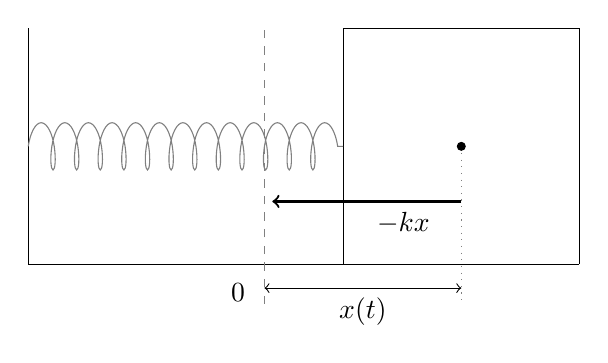
\begin{tikzpicture}
\draw[-] (0,0) -- (7,0);
\draw[-] (0,0) -- (0,3);

\draw[-] (4,0) -- (4,3) -- (7,3) -- (7,0);

\draw[gray,dashed] (3,-0.5) -- (3,3);
\draw[gray,dotted] (5.5,1.5) -- (5.5,-0.5);
\draw[thick,->] (5.5,0.8) -- node[below right, fill=white] {$-kx$} (3.1,0.8);
\node[label=below left:{$0$}] at (3,0) {};

\draw[gray,decoration={aspect=0.3, segment length=3mm, amplitude=3mm,coil},decorate] (0,1.5) -- (4,1.5);

\draw[<->] (3,-0.3) -- node[below] {$x(t)$} (5.5,-0.3);
\node[draw, fill=black, circle, inner sep=1pt] at (5.5,1.5) {};
\end{tikzpicture}
\caption{Sistema masa-resorte, con la fuerza del muelle $-kx$.}
\label{imgMasaResorte1}
\end{figure}

Según la ley de Hooke, la fuerza será

\[ F = -kx \]

donde $k$ es una constante que depende del muelle. Por la segunda ley de newton, tenemos que la fuerza es el producto de la masa y la aceleración, por tanto, la ecuación que describe el movimiento es

\[ mx'' = -kx \]

Podemos transformarla a un problema en derivadas ordinarias

$$\left\lbrace \begin{array}{l}
x'' + \frac{k}{m}x = 0\\
x(0) = x_0\\
x'(0) = v_0
\end{array}\right. $$

para el que necesitaremos posición y velocidad iniciales.

El polinomio característico es

\[ λ^2 + \frac{k}{m} = 0 \]

cuyas raíces son

\[ λ=\pm \imath \sqrt{\frac{k}{m}} \]

Las soluciones complejas son, por lo tanto,

\begin{gather*}
z_1 = e^{\imath t\sqrt{\frac{k}{m}}} = \cos \sqrt{\frac{k}{m}} t + \imath\sin \sqrt{\frac{k}{m}} t \\
z_1 = e^{-\imath t\sqrt{\frac{k}{m}}} = \cos \sqrt{\frac{k}{m}} t - \imath\sin \sqrt{\frac{k}{m}} t 
\end{gather*}

Combinándolas de forma lineal, obtenemos dos soluciones reales:

\begin{gather*}
x_1(t) = \Re (z_1) = \cos \sqrt{\frac{k}{m}} t \\
x_2(t) = \Im (z_1) = \sin \sqrt{\frac{k}{m}} t
\end{gather*}

Aunque se ve a simple vista que esas dos soluciones son independientes (el coseno y el seno del mismo ángulo), deberíamos calcular el Wronskiano para comprobar que son realmente independientes.

La solución general nos queda

\begin{equation}\label{eqMasaResorte} x(t) = A\cos \sqrt{\frac{k}{m}} t + B \sin \sqrt{\frac{k}{m}} 
\end{equation}

Las constantes $A$ y $B$ se tendrán que obtener una vez dados los valores iniciales. Si suponemos $x(0) = x_0$, $x'(0) = v_0$, tenemos que

\begin{align*}
x_0 &= x(0) = A \\
x'(t) &= -x_0 \sqrt{\frac{k}{m}} \sin \sqrt{\frac{k}{m}} t + B \sqrt{\frac{k}{m}}\cos\sqrt{\frac{k}{m}} t \\
v_0 &= x'(0) = B \sqrt{\frac{k}{m}} \\
B &= \frac{v_0}{\sqrt{\frac{k}{m}}}
\end{align*}

Si bien esta solución es correcta, los físicos suelen reescribirla de una forma distinta utilizando coordenadas polares para el punto $(A,B)$:

\begin{align*}
A &= R\cos φ \\
B &= R\sin φ
\end{align*}

Sustituyendo en \eqref{eqMasaResorte}

\[ x(t) = R\left(\cos \sqrt{\frac{k}{m}} t\cos φ + \sin \sqrt{\frac{k}{m}} t \sin φ \right) = R\cos\left(\sqrt{\frac{k}{m}}t - Φ\right) \]

donde $Φ = \arctan \frac{B}{A}$ es el desfase, que actúa de velocidad inicial del sistema.

\paragraph{Sistema masa-resorte con rozamiento}

Replanteemos el problema anterior con rozamiento.
\begin{figure}
\centering
\begin{tikzpicture}
\draw[-] (0,0) -- (7,0);
\draw[-] (0,0) -- (0,3);

\draw[-] (4,0) -- (4,3) -- (7,3) -- (7,0);

\draw[gray,dashed] (3,-0.5) -- (3,3);
\draw[gray,dotted] (5.5,1.5) -- (5.5,-0.5);
\draw[thick,->] (5.5,2) -- node[above right, fill=white] {$-εx'$} (2.7,2);
\draw[thick,->] (5.5,0.8) -- node[below right, fill=white] {$-kx$} (3.1,0.8);
\node[label=below left:{$0$}] at (3,0) {};

\draw[gray,decoration={aspect=0.3, segment length=3mm, amplitude=3mm,coil},decorate] (0,1.5) -- (4,1.5);

\draw[<->] (3,-0.3) -- node[below] {$x(t)$} (5.5,-0.3);
\node[draw, fill=black, circle, inner sep=1pt] at (5.5,1.5) {};
\end{tikzpicture}
\caption{Sistema masa-resorte con rozamiento (fuerza $-εx'$).}
\end{figure}

La ecuación cambia al añadir el rozamiento:

\begin{gather} mx'' = -kx - εx' \nonumber \\
x'' + \frac{ε}{m}x' + \frac{k}{m}x = 0
\end{gather}

Resolvemos el polinomio característico \[ λ^2 + \frac{ε}{m}λ + \frac{k}{m} = 0 \] y nos queda

\[ λ = \frac{-ε}{2m} \pm \sqrt{\left(\frac{ε}{2m}\right)^2 - \frac{k}{m}} \].

Tenemos que plantear tres casos basados en el valor de $Δ =\left(\frac{ε}{2m}\right)^2 - \frac{k}{m}$: si es mayor, igual o menor que cero.

\subparagraph{Primer caso: $Δ > 0$ (rozamiento alto)}

Tenemos

\begin{gather*}
λ_+ = \frac{-ε}{2m} + \sqrt{\left(\frac{ε}{2m}\right)^2 - \frac{k}{m}} \\
λ_- = \frac{-ε}{2m} - \sqrt{\left(\frac{ε}{2m}\right)^2 - \frac{k}{m}} 
\end{gather*}

De sus expresiones vemos que tanto $λ_+$ como $λ_-$ son negativos, puesto que la raíz siempre será menor que $\frac{\epsilon}{2m}$. La solución general del problema es

\[ x(t) = Ae^{λ_+t} + Be^{λ_-t} \]

Despejando de los valores iniciales $x(0) = x_0$, $x'(0) = v_0$ y realizando ciertas operaciones,

\[ x(t) = \frac{1}{λ_+ - λ_-}\left((v_0-λ_-x_0)e^{λ_+t} - (v_0-λ_+x_0)e^{λ_-t}\right) \]

De esa ecuación vemos que, cuando $t\to ∞$, $x(t) \to 0$. Es decir, el objeto tiende a pararse.

También querríamos ver cuántas veces pasamos por la posición de equilibrio. Tenemos que resolver la ecuación

\[ e^{(λ_+ - λ_-)t} = \frac{v_0-λ_+x_0}{v_0-λ_-x_0} \]

que no tiene solución (la exponencial es siempre positiva, pero la división es menor que 1). Por lo tanto, el objeto no llega nunca a la posición de equilibrio.

\subparagraph{Segundo caso: $Δ=0$}

En este caso, tenemos $λ=\frac{-ε}{2m}$ que es una raíz doble. Por el método de variación de las constantes, nuestras dos soluciones son

\[ x_1(t) = e^{\frac{-ε}{2m}t};\quad x_2(t) = te^{\frac{-ε}{2m}t} \]

y la solución general se expresa como

\[ x(t) = A e^{\frac{-ε}{2m}t} + B t e^{\frac{-ε}{2m}t} = e^{\frac{-ε}{2m}t} \left(A + Bt\right) \]

Al igual que en el anterior caso, $x(t) \convs[][t][∞] 0$, pero aquí sí que podemos tener soluciones para $x(t) = 0$. La existencia o no de una solución dependerá de la posición y velocidad iniciales.

\subparagraph{Tercer caso: $Δ < 0$ (sin rozamiento)}

Aquí tendremos raíces complejas, es decir:

\[ λ_+ = \frac{-ε}{2m} + \imath\sqrt{\frac{k}{m} - \left(\frac{ε}{2m}\right)^2} \]

y su conjugada. De esta forma, las dos soluciones reales serán

\begin{gather*}
x_1(t) = e^{\frac{-ε}{2m}t} \cos t\sqrt{\frac{k}{m} - \left(\frac{ε}{2m}\right)^2} \\
x_1(t) = e^{\frac{-ε}{2m}t} \sin t\sqrt{\frac{k}{m} - \left(\frac{ε}{2m}\right)^2} \\
\end{gather*}

Podemos extraer la solución general y hacer el cambio del anterior apartado, pasando a polares $(A,B) \sim (R\cos φ, R\sin φ)$, de tal forma que nos queda la solución general

\[ x(t) = R e^{-\frac{ε}{2m}t} \cos \left(t\sqrt{\frac{k}{m} - \left(\frac{ε}{2m}\right)^2} - φ\right) \]

Es decir, hay un decaimiento exponencial de la amplitud. La gráfica de la función sería la de la \textbf{Figura \ref{fig:imgMasaResorteSeno}}

\img{img/MasaResorteSeno.png}{$x(t)$ para un sistema masa-resorte}{imgMasaResorteSeno}{0.8}

\paragraph{Péndulo simple}

Consideramos un péndulo simple sin rozamiento.

\begin{figure}[hbtp]
\centering
\begin{tikzpicture}
\node (O) at (0,0) {};
\node (Vert) at (0,-2) {};
\node (P) at (1,-2) {};

\draw[-] (-2,0) -- (2,0);
\draw[-] (0,1) -- (O.center);
\draw[dashed] (O.center) -- (0,-4);

\draw[-] (O.center) -- (P.center);
\draw[->] (P.center) -- node[right] {$mg$} (1,-3.5);
\node[draw, fill=gray, circle, inner sep=4pt] at (P) {};

\tikzangle[name=$\theta$]{O.center}{P.center}{Vert.center}
\end{tikzpicture}
\caption{El péndulo}
\end{figure}

Tenemos las ecuaciones de posición

\[ σ(t) = (L\sin θ(t), - L \cos θ(t))\]

de velocidad

\[ σ'(t) = (Lθ'(t)\cos θ(t), Lθ'(t)\sin θ(t))\]

y aceleración

\begin{align*}
 σ''(t) = (&-L(θ'(t))^2\sin(t) + Lθ''(t)\cos(t), \\
 & L(θ'(t))^2\cos θ(t) + Lθ''(t)\sin θ(t)) 
 \end{align*}.

Por la segunda ley de Newton, tenemos que la fuerza ejercida es igual al producto de la masa y la aceleración. Si dividimos la cuerda en su componente tangencial y perpendicular tenemos:

\[ mg( -\cosθ, -\sin θ)\sin θ  = m σ''(t) \]

y por lo tanto nos quedan las dos ecuaciones
\[
\left\{\begin{matrix}
 -g\sin θ \cos^2 θ = -L θ'^2 \cos θ \sin θ+ Lθ''\cos^2θ  \\
 -g\sin θ \sin^2 θ = -L θ'^2 \sin θ \cos θ  + Lθ''\sin^2θ  
 \end{matrix}\right\} \]

 La ecuación final es \[ -g\sin θ = L θ'' \] o, transformada

 \[ θ'' + \frac{g}{L} \sin θ = 0 \]

Por Taylor, podemos aproximar $\sin θ \sim θ$ cuando θ es pequeña, de tal forma que nos reducimos al caso de un sistema masa-resorte.

\subsection{Problemas lineales no homogéneos con coeficientes constantes}

¿Qué ocurre cuando consideramos sistemas con fuerzas externas? Un ejemplo sería la siguiente ecuación en orden dos:

\begin{equation}
\label{eqEcOrden2} x'' + ax' + bx = f(t)
\end{equation}

en la que $f(t)$ representa esa fuerza externa. Tal y como habíamos visto en anteriores secciones, la solución general $X_G$ se escribía como una solución particular $X_P$ más todas las asociadas al homogéneo $X_H$. En esta situación el problema es encontrar la solución particular, para lo cual teníamos varios métodos.

\subsubsection{Método de variación de constantes}
\label{secMetodoVarConst}
\index{Variación!de constantes}

Siguiendo con el ejemplo en orden 2, tenemos

\[ x_H (t) = c_1x_1(t) + c_2x_2(t) \]
y buscamos una solución en la que
$$
\left\lbrace
\begin{array}{l}
c_1 = c_1(t)\\
c_2 = c_2(t)
\end{array}
\right.
$$
Por tanto buscamos $X_P$ tal que
\[ x_P(t) = c_1(t)x_1(t) + c_2(t)x_2(t) \] Para ello derivamos:
\begin{align*}
x_P'&= c_1'x_1 + c_1x_1' + c_2'x_2 + c_2x_2' \\
x_P'' 	&= c_1''x_1+c_1'x_1' + c_2''x_2+c_2'x_2' + \\
		&\quad+ c_1'x_1'+c_1x_1'' + c_2'x_2' + c_2x_2'' = \\
		&= c_1''x_1 + c_2''x_2+2c_1'x_1'+2c_2'x_2' + c_1x_1'' +c_2x_2''
\end{align*}

Sustituyendo en \eqref{eqEcOrden2}:

\begin{align*}
f(t) &= x_P'' + ax_P' + bx_P = &  \\
	&= c_1''x_1 + c_2''x_2 + 2c_1'x_1' + 2c_2'x_2'  + c_1x_1''  + c_2x_2'' \\
	& + ac_1' x_1 + ac_2'x_2  + ac_1x_1'  + ac_2x_2' \\
	&  + bc_1x_1  + bc_2x_2 
\end{align*}

Tras la sustitución tenemos una expresión bastante compleja. Sin embargo, recordamos que no buscamos todas las soluciones de la ecuación, sino que basta con encontrar sólo una. Por ello, planteamos ciertas condiciones para resolver la expresión hallada:

$$ \left\lbrace \begin{array}{l}
c_1'x_1 + c_2'x_2 = 0 \\
c_1'x_1' + c_2'x_2' = f
\end{array} \right. $$
Que nos lleva al sistema

\[ \underbrace{\begin{pmatrix}
x_1 & x_2 \\
x_1' & x_2'
\end{pmatrix}}_A\begin{pmatrix}
c_1' \\ c_2'
\end{pmatrix} = \begin{pmatrix}
0 \\ f(t)
\end{pmatrix} \]
Se puede observar que el sistema tiene solución, ya que al ser $x_1,\ x_2$ soluciones independientes, el Wronskiano (en este caso, el determinante de $A$) es distinto de $0$.

En un caso general de orden $n$, el sistema a plantear tendrá la siguiente forma

\[ \begin{pmatrix}
x_1 & \cdots & x_n \\
x_1' & \cdots & x_n \\
\vdots & \ddots & \vdots \\
x_1^{n-1)} & \cdots & x_n^{n-1)}
\end{pmatrix} \begin{pmatrix} c_1' \\ c_2' \\ \vdots \\ c_n' \end{pmatrix}
=
\begin{pmatrix}
0 \\ \vdots \\ 0 \\ f(t)
\end{pmatrix} \]
Veamos un ejemplo.

\begin{example}
$x'' + x = e^t$

Buscamos $x_P(t) = c_1(t) x_1 + c_2(t) x_2$, donde

\[ \underbrace{\begin{pmatrix}
x_1 & x_2 \\
x_1' & x_2'
\end{pmatrix}}_A\begin{pmatrix}
c_1' \\ c_2'
\end{pmatrix} = \begin{pmatrix}
0 \\ e^t
\end{pmatrix} \]

Podemos elegir $x_1$ y $x_2$ como el seno y el coseno de $t$:

\[ \underbrace{\begin{pmatrix}
\cos t & \sin t \\
- \sin t & \cos t
\end{pmatrix}}_A\begin{pmatrix}
c_1' \\ c_2'
\end{pmatrix} = \begin{pmatrix}
0 \\ e^t
\end{pmatrix} \]
Resolviendo el sistema nos queda que

\[ c_2' = e^t \cos t \]

Realizando bastantes operaciones podemos obtener una solución particular, sin embargo, podemos darnos cuenta de que una de las soluciones particulares es

\[ x_p(t) = \frac{e^t}{2} \]

¿Qué tiene de especial este problema? La exponencial en $f(t)$. Lo que nos lleva a estudiar otro método, el de coeficientes indeterminados.
\end{example}


\subsubsection{Método de coeficientes indeterminados}

Podremos aplicar este método cuando $f(t)$ sea un polinomio, una exponencial, senos y cosenos y combinaciones lineales de todos los anteriores. En todos estos casos las derivadas nos llevan a funciones de la misma clase, y podremos aplicar este método que nos lleva a cuentas más sencillas.

En este método, suponemos que la solución particular es una función de la misma familia de $f(t)$ multiplicada por una constante, así que planteamos el problema y resolvemos el sistema. Estudiémoslo desde un ejemplo:

\paragraph{1) Exponenciales} \[ x'' - x = e^{2t} \]

Tenemos que
\begin{gather*}
x_p(t) = Ce^{2t} \\
x_p' = 2Ce^{2t} \\
x_p'' = 4Ce^{2t} \\
e^2t = 4Ce^{2t} - Ce^{2t} = 3Ce^{2t}
\end{gather*}

$C$ ha de ser $\frac{1}{3}$ y por lo tanto nuestra solución general del sistema será

\[ x_G = c_1e^t + c_2e^{-t} + \frac{1}{3}e^{2t} \]

\paragraph{2) Exponenciales con $f(t)$ solución de la homogénea} Otro ejemplo:

\[ x''-x= e^t \]

Aquí habría que calcular $x_p = ce^t$. Sin embargo, tomando esa solución nos quedaría $x_p'' - x_p = 0\; ∀c$, por lo que no nos vale. Cuando $f(t)$ es una de las soluciones de la ecuación homogénea asociada, tenemos que añadir algo más. Buscamos soluciones de la forma $cte^t$

\begin{gather*}
x_p  = cte^t \\
x_p' = cte^t + ce^t \\
x_p'' = cte^t + 2ce^t \\
\end{gather*}

Resolviendo:

\begin{align*}
x_p'' - c_p &= 2ce^t \\
e^t &= 2ce^t \\
C &= \frac{1}{2}
\end{align*}

\paragraph{3) Senos y cosenos} Probamos ahora con senos y cosenos.

\[ x'' + x= \cos 2t\]

En este caso, la solución debe tener una combinación lineal de senos y cosenos. Por lo tanto

\[ x_p = A\cos 2t + B\sin 2t \]

y resolviendo

\[ \cos 2t = x_p'' + x_p = -3A\cos 2t - 3B\sin 2t \]

de tal forma que $A=\frac{-1}{3}$ y $B=0$.

\paragraph{4) Senos y cosenos con $f(t)$ sol. de la homogénea} Consideramos $x''+x = \cos t$.

En este caso, $f(t) = \cos t$ es una solución de la parte homogénea, así que la solución será de la forma

\[ x_p(t) = At\cos t + Bt\sin t \]

Supongamos que esto modela una situación real, como por ejemplo empujando un columpio. ¿Cómo interpretamos esto?

A ciertas frecuencias, la ecuación es creciente, la amplitud aumenta con el tiempo. Es un fenómeno de \textbf{resonancia}. Veamos cómo modelizar este caso.

\paragraph{Ejemplo: Sistema masa-resorte con fuerza externa (sin rozamiento)}

La ecuación en este caso es

\(\label{eqMRF1} x'' + \underbrace{\frac{k}{m}}_{=ω^2}x = \underbrace{f(t)}_{F\cos αt} \)

Hemos cambiado algunas constantes para adaptarlo a nuestro caso. Hay varias opciones a partir de aquí relacionadas con las constantes ω y α:

\subparagraph{Caso 1: $ω≠α$}

Resolvemos la ecuación homogénea $x''+ω^2 x = 0$ con el polinomio característico:

\[ λ^2+ω^2  = 0 \implies λ = \pm ω\imath \]

y por lo tanto

\( x_H(t) = c_1 \cos ωt + c_2 \sin ωt \)

Necesitamos ahora una solución particular $x_P = A\cos αt + B\sin αt$. Derivamos dos veces:

\begin{align*}
x_P(t) &= A\cos αt + B\sin αt \\
x_P'(t) &= -Aα\sin αt + Bα\cos αt \\
x_P''(t) &= -Aα^2\cos αt - Bα^2\sin αt 
\end{align*}

Sustituyendo en \eqref{eqMRF1}

\begin{gather*}
 F\cos αt = x_P'' + ω^2x_P = \dotsb = (ω^2-α^2)\left(A\cos αt + B\sin αt\right) \\
 B = 0;\quad A= \frac{F}{ω^2-α^2} \\
 x_P(t) = \frac{F}{ω^2-α^2}\cos αt
\end{gather*}

De esta forma, la ecuación general nos queda

\( x_G(t) = \frac{F}{ω^2-α^2}\cos αt + c_1 \cos ωt + c_2 \sin ωt \)

Para los datos iniciales $x(0) = x'(0) = 0$, despejamos y tenemos la solución al problema

\(\label{eqMRF2-Sol} x(t) = \frac{F}{ω^2-α^2}\left(\cos αt - \cos ωt\right) \)

Volviendo de nuevo al sistema que tratamos, ω y α representan dos frecuencias. α es la externa y ω es la natural. Podemos reescribir la ecuación \eqref{eqMRF2-Sol} usando identidades trigonométricas. Sabemos que

\[ \cos (A-B) - \cos(A+B) = 2\sin A \sin B \]

Resolvemos:

\[ \left.\begin{matrix}A - B = αt \\ A + B = ωt \end{matrix}\right\}
\left.\begin{matrix}A = \frac{ω+α}{2}t \\ B = \frac{ω-α}{2}t\end{matrix}\right\} \]

Sustituyendo en \eqref{eqMRF2-Sol}:

\( x(t) = \frac{2F}{ω^2-α^2} ·\sin\left( \frac{ω-α}{2}t\right) · \sin\left( \frac{ω+α}{2}t\right)  \)

Luego lo que tenemos es una oscilación rápida (Δ) con una amplitud contenida dentro de otra con oscilación más lenta (Γ).

\begin{figure}
\centering
\includegraphics[width=0.8\textwidth]{img/MasaResorteF.png}
\caption{Gráfico de una oscilación rápida (Δ, azul) con una amplitud contenida dentro de otra con oscilación más lenta (Γ, verde)}
\label{imgMasaResorteF}
\end{figure}

\subparagraph{Caso 2: $ω=α$}

En este caso, la ecuación diferencial es

\[ x'' + ω^2 x = F\cos ωt \]

La solución de la homogénea es $x_H = c_1 \cos ωt + c_2 \sin ωt$. Tenemos un problema: $F\cos ωt$ es solución de la homogénea. Para encontrar una solución particular multiplicamos entonces por $t$:

\begin{gather*}
x_P = t\left(A\cos ωt + B\sin ωt\right) \\
x_P' =t\left(-Aω\sin ωt + Bω\cos ωt\right) + \left(A\cos ωt + B\sin ωt\right) \\
x_P'' = t\left(-Aω^2 \cos ωt - Bω^2 \sin ωt\right) + 2\left(-Aω\sin ωt + Bω\cos ωt \right)
\end{gather*}

Igualando,

\[ F\cos ωt \stackrel{?}{=} x_p'' + ω^2x_p = 2\left(-Aω\sin ωt + Bω\cos ωt \right) \]

de donde sacamos que $A=0$ y $B=\frac{F}{2ω}$. Una solución particular es entonces

\[ x_P(t) = \frac{F}{2ω}t \sin ωt \]

que es además la solución que cumple $x_P(0) = x_P'(0) = 0$. La gráfica de esta ecuación será

\begin{figure}[hbtp]
\centering
\includegraphics[width=0.5\textwidth]{img/MasaResorteF-Resonancia.png}
\caption{Gráfica de un sistema masa-resorte en resonancia}
\label{imgMasaResorteFR}
\end{figure}

Estamos ante un fenómeno de resonancia. La amplitud tiene a infinito siempre, por muy pequeña que sea la fuerza.

Que, por cierto, Azorero nos ha engañado en una cosa: la expresión de la fuerza es un coseno en lugar de una función genérica $F(t)$. En realidad esto se debe al desarrollo en serie de Fourier, que dice que cualquier función se puede expresar como

\[ F(t) = \sum_{j=0}^∞ F_j \cos \frac{jπ}{T}t \]

\paragraph{Modelo con rozamiento}

Añadiendo el rozamiento al modelo anterior, tenemos

\[ x''+2εx'+ω^2x = \cos αt \]

Haciendo cuentas y suponiendo $ε^2-ω^2<0$. Nos queda una solución para la homogénea

\[ x_H = e^{-εt}\left(c_1 \cos \left( \sqrt{ω^2-ε^2}t \right) + c_2 \sin \left( \sqrt{ω^2-ε^2}t\right)\right) \]

Buscamos la solución particular

\[ x_P (t) = A\cos αt + B\sin αt \]

y llegamos a

\[ x_P(t) = \frac{1}{(ω^2-α^2)^2 + 4α^2ε^2}\left((ω^2-α^2)\cos αt + 2αε \sin αt \right) \].

La solución general es entonces

\[ x_G(t) = x_P(t) + x_H(t) \]

Dado que en $x_H$ está todo multiplicado por una exponencial negativa, tiende a cero cuando $t\to ∞$, por lo que la llamamos la parte \textbf{transitoria}. El primer sumando, $x_P$, permanece y se le llama la parte \textbf{estacionaria}.

En este caso, cuando $α=ω$ (estamos en la frecuencia de resonancia), es el que más aporta a la ecuación. Sin embargo, en ningún caso la amplitud se va a infinito. El rozamiento impide que la amplitud se dispare.

\subsubsection{Resumen de métodos para ec. lineales no homogéneas}

Hagamos un resumen de los métodos que hemos visto. Las soluciones de una ecuación no homogénea de la forma

\[ y^{n)} + a_{n-1}y^{n-1)} + \dotsb + a_1y'+a_0y = f(t) \]

se expresan en función de una solución particular $y_p$ y el conjunto de las soluciones para la ecuación homogénea asociada $y_H$:

\[ y_G = y_p + y_H \]

Podemos obtener fácilmente las soluciones a la homogénea usando la técnica vista en la sección anterior \eqref{secEcHomoLinealConstante}. Para obtener la solución particular tenemos que usar el método de variación de constantes (\ref{secMetodoVarConst}). Sin embargo, ese método nos lleva a muchas más cuentas de las necesarias. Podemos simplificar las cosas cuando $f(t)$ pertenece a una familia de curvas "cerrada" por la derivada. Veamos esos casos.

\paragraph{Polinomio}

\[ f(t) = A_0 + A_1t + \dotsb + A_Nt^N \]

Si $0$ no es raíz, buscamos \[y_p(t) = a_0 + a_1t + \dotsb + a_Nt^N\]. Si $0$ es raíz con multiplicidad $k$, entonces la solución particular que buscamos será de la forma

\[ y_p(t) =( a_0 + a_1t + \dotsb + a_Nt^N)t^k \]

\paragraph{Trigonométrico}

\[ f(t) = \cos αt \]

o análogamente para senos. Tenemos dos posibilidades. Si $α\i$ no es raíz del p. característico, la solución particular es de la forma

\[ y_p(t) = a\cos αt + b\sin αt \]

En el caso de que $α\imath$ sea raíz con multiplicidad $k$, entonces

\[ y_p(t) = (a\cos αt + b\sin αt)t^k \]

\paragraph{Polinomio y exponencial}

\[ f(t) = e^{αt}(A_0 + A_1t + \dotsb + A_Nt^N) \]

Si $α$ no es raíz del p. característico,

\[ y_p(t) = e^{αt}(a_0 + a_1t + \dotsb + a_Nt^N) \]. si α sí es raíz con multiplicidad $k$,

\[ y_p(t) = t^ke^{αt}(a_0 + a_1t + \dotsb + a_Nt^N) \]

\subsection{Ejemplos}

\begin{example} Consideramos la ecuación

\[ y'' + a' + by = 0 \]

Demuestra que

\[ y_H(t) \convs[][t][∞] 0 \iff a>0, b>0 \]

Empezamos por la implicación a la izquierda. El polinomio característico es

\[ λ^2+aλ+b \implies λ_{\pm} = \pm \frac{a\pm \sqrt{a^2-4b}}{2} \]

Tenemos tres casos:

\begin{itemize}
\item $a^2-4b > 0$. En este caso, $λ_-,λ_+ ∈ℝ$, $λ_-<λ_+<0$ y por lo tanto $e^{λ_+t}$ y $e^{λ_-t}$ tienden a cero cuando $t\to ∞$.

\item $a^2=4b$. Aquí tenemos que $λ=\frac{-a}{2}$, raíz doble. Las soluciones son $e^{\frac{-a}{2}t}$ y $te^{\frac{-a}{2}t}$, ambas tienden a cero.

\item $a^2-4b > 0$. Las raíces son imaginarias y te sale igual porque lo ha borrado.

\end{itemize}

Para demostrar la implicación a la derecha, tenemos que si $y_H(t)\convs[][t][∞]0$, entonces los autovalores del p.c. son o bien

\[ y_\pm = α\pm + \iβ \]

con $α<0$ o bien reales con $λ_-≤λ_+<0$. En ambos casos tenemos que $a>0, b>0$ tal y como hemos visto al demostrar la otra implicación.

\end{example}

\begin{example}[Ejercicio 7]

Tenemos la siguiente ecuación:

\[ y^{iv)} + 4y''' + 8y'' + 8y' +4y = 0\]

y nos dicen que $\imath- 1$ es raíz del p.c.

\[ P(λ) = λ^4 + 4λ^3 + 8λ^2 + 8λ + 4 = 0 \]

Sabiendo que $\i-1$ es raíz y que su conjugado $-\imath- 1$ también, podemos hacer las cuentas y

\begin{gather*}
 P(λ) = (λ-(-1+\i)) · (λ-(-1-\i)) · P_2(λ) \\
 ((λ+1)^2 + 1) P_2(λ)
 \end{gather*}

donde

\[ P_2(λ) = \frac{λ^4+ 4λ^3 + 8λ^2 + 8λ + 4 }{λ^2+2λ + 2} = \dotsb = λ^2 + 2λ + 2 \].

Por lo tanto las dos raíces son dobles.
\end{example}

\begin{example}[Ejercicio 8] Tenemos la ecuación

\[ y^{n)} + a_{n-1}y^{n-1)} + \dotsb + a_1y' + a_0y = x^k \]

con $a_0≠0$. Demostrar que en el caso $n=4,k=3$, existe un único polinomio que sea solución del problema, que además tiene grado 3.

Hay que demostrar dos cosas: que existe y que es único. Empezamos demostrando la unicidad suponiendo que existen $P,Q$ polinomios de grado tres solución.

En este caso tendríamos que $P-Q$ es solución de la homogénea. Y ha dicho algo y no lo he podido copiar.

Demostramos ahora la existencia. Buscamos una solución polinómica $y(x) = c_0+c_1x + c_2x^2 + c_3x^3$. Si calculamos

\[ a_0y(x) + a_1y'(x) + a_2y''(x) + a_3y'''(x) = x^3 = \underbrace{\{c_j,a_j\}}_{=0} + \underbrace{\{c_j,a_j\}x}_{=0} + \underbrace{\{c_j,a_j\}x^2}_{=0} + \underbrace{\{c_j,a_j\}}_{=1}x^3 \]

donde $\{c_j,a_j\}$ son combinaciones lineales de cada una de las $a_j$ y $c_j$. Tendremos entonces un sistema con coeficientes $a_j$ e incógnitas $c_j$ de la forma

\[ A \begin{pmatrix}
c_0 \\ c_1 \\ c_2 \\ c_3
\end{pmatrix} = \begin{pmatrix}
0 \\ 0 \\ 0 \\ 1
\end{pmatrix} \]
\end{example}

\begin{example}[Ejercicio 11 - Hoja 3]

Tenemos la ecuación

\[ y'' + P(t) y' + Q(t) y = 0 \]

Decir sobre qué condiciones de $P,Q$ el cambio de variables $s=Φ(t), z(s) = y(t)$ convierte la ecuación en una coeficientes constantes.

Calculamos las derivadas:

\begin{gather*}
 \od{y}{t} = \od{y}{t} \od{s}{t} = \od{z}{s} \od{Φ}{t} \\
 \od[2]{y}{t} = \od[2]{z}{s} \left(\od{Φ}{t}\right)^2 + \od{z}{s}\od[2]{Φ}{t}
\end{gather*}

y sustituyendo

\[ 0 = \od[2]{z}{s} + \underbrace{\left(\frac{\od[2]{Φ}{t} + P\od{Φ}{t}}{\left(\od{Φ}{t}\right)^2}\right)}_{A} \od{z}{s} + \underbrace{\frac{Q}{\left(\od{Φ}{t}\right)^2}}_{B}z \]

tenemos que buscar las condiciones sobre $P$ y $Q$ y la expresión de $Φ(t)$ para que ahí haya constantes multiplicando a $\od{z}{s}$ y a $z$. Entonces

\[ \frac{Q}{\left(\od{Φ}{t}\right)^2} = B \implies \left(\od{Φ}{t}\right)^2 = \frac{Q}{B} \implies \od{Φ}{t} = \sqrt{\frac{Q}{B}} \]

Sustituyendo:

\[ A = \frac{\od[2]{Φ}{t} + P\sqrt{\frac{Q}{B}}}{\left(\od{Φ}{t}\right)^2} \]

Casi tenemos la relación, pero tenemos que deshacernos de esa segunda derivada. Así que derivamos Φ:

\[ \od[2]{Φ}{t} = \frac{A}{2\sqrt{B}\sqrt{Q}}Q' \]

y sustituimos

\[ A = \frac{\frac{1}{2\sqrt{B}\sqrt{Q}}Q' + P\sqrt{\frac{Q}{B}}}{\left(\od{Φ}{t}\right)^2} = \dotsb = \frac{Q'+2PQ}{Q\sqrt{Q}} = \text{cte.} \]

y además tiene que ser

\[ (Φ'(t))^2 = \frac{Q(t)}{B} \]

\end{example}


\section{Teoremas de existencia y unicidad}

Partiendo del problema

\[ \begin{cases}
y' = f(x,y(x)) \\
y(x_0) = y_0
\end{cases} \]

podemos hacer una \textbf{formulación integral equivalente} de la forma

\[ y(x) = y_0 + \int_{x_0}^x f(s,y(s))\dif s \].

Hay dos posibles aproximaciones para resolver este problema.

\paragraph{Iteradas de Picard}\index{Iteradas!de Picard} Veamos este método con un ejemplo. Partimos de 

\[ \begin{cases}
y' = y \\
y(x_0) = 1
\end{cases} \].

La primera aproximación será

\[ y_1(x) = 1 + \int_0^x y_0 \dif x = 1+ \int_0^x 1\dif s = 1 + x \]. Hacemos una segunda aproximación:

\[ y_2(x) = 1 + \int_0^x y_1 \dif x = 1 + \int_0^x 1+s \dif s  = 1 + x +\frac{x^2}{2} \]

Podríamos seguir haciendo iteradas basándonos en la misma fórmula

\(\label{eqIteradasPicard} y_n(x) = 1 + \int_0^x y_{n-1}(s) \dif s \)

y veríamos que lo que sale es el polinomio de Taylor de la exponencial\footnote{No es cierto que el método de Picard dé siempre el desarrollo de Taylor. Es una casualidad de este ejemplo.}. Planteamos entonces un algoritmo iterativo siguiendo la ecuación \eqref{eqIteradasPicard}. Si consiguiésemos demostrar que

\begin{itemize}
\item $y_n(x) \convs[][n] y(x)$.
\item $\displaystyle\lim_{n\to\infty} \int_{x_0}^x f(s,y_{n-1}(s))\dif s = \int_{x_0}^x \lim_{n\to ∞} f(s,y_{n-1}(s)) \dif s$.
\item $\displaystyle\lim_{n\to ∞} f(s, y_{n-1}(s)) = f(s,y(s))$.
\end{itemize}

tendríamos siempre una solución al problema. Sin embargo, no es trivial definir qué es un límite de funciones, entrando dentro del análisis funcional. Además, deberíamos ver hasta qué $x$ podríamos usar la solución. 

Buscamos por lo tanto otro método para resolver el problema.

\paragraph{Método de las poligonales de Euler}\index{Poligonales!de Euler} Supongamos que la solución exacta del problema es $y(x)$. Entonces, para un $x_1=x_0 + h$, podemos decir que

\[ y(x_1) = y(x_0 + h) \stackrel{\text{Taylor}}{=} y(x_0) + y'(x_0)\cdot h + \mop{error}(h) \]

Ahora bien, sabemos que $y(x_0) = y_0$ y que $y'(x_0) =f(x_0, y_0)$. Entonces

\[ y(x_1) ≈ y_0 + f(x_0, y_0)·h \equiv y_1 \]

es un valor aproximado de la solución en $x_1$. Repetimos el proceso. Tomamos $x_2 = x_1 + h$, y 

\[ y(x_2) ≈ y_1 + f(x_1,x_1)· h \equiv y_2 \]

Rehaciendo el proceso, llegamos a una poligonal $P_n$ (poligonal de Euler) que aproximará la curva:

\begin{figure}[hbtp]
\centering
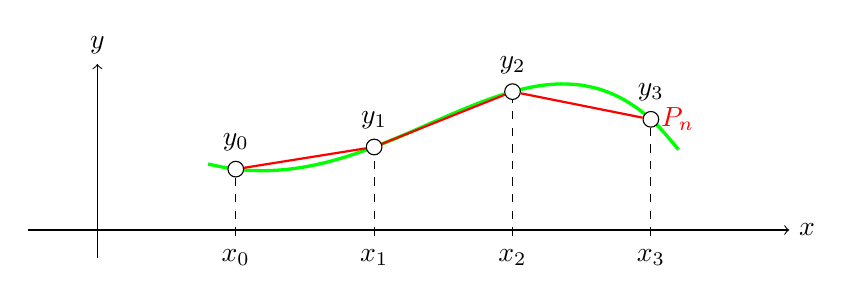
\begin{tikzpicture}[x=50pt,y=20pt]
	\draw[->] (-0.5,0) -- (5,0) node[right] {$x$};
	\draw[->] (0,-0.5) -- (0,3) node[above] {$y$};
	
	\draw[very thick,domain=0.8:4.2,smooth,variable=\x,green] plot ({\x},{2.19805 - 1.84594*\x + 0.64716*\x*\x + 0.150811*\x*\x*\x - 0.0500811*\x*\x*\x*\x});
	
	\node[draw,label=above:{$y_0$},circle, fill=white, inner sep=2pt] (A) at (1,1.1) {};
	\node[draw,label=above:{$y_1$},circle, fill=white, inner sep=2pt] (B) at (2,1.5) {};
	\node[draw,label=above:{$y_2$},circle, fill=white,inner sep=2pt] (C) at (3,2.5) {};
	\node[draw,label=above:{$y_3$},circle, fill=white, inner sep=2pt] (D) at (4,2) {};
	
	\node[label=below:{$x_0$}] at (1,0) {};
	\node[label=below:{$x_1$}] at (2,0) {};
	\node[label=below:{$x_2$}] at (3,0) {};
	\node[label=below:{$x_3$}] at (4,0) {};
	
	\draw[-, dashed] (1,-0.1) -- (A);	
	\draw[-, dashed] (2,-0.1) -- (B);
	\draw[-, dashed] (3,-0.1) -- (C);
	\draw[-, dashed] (4,-0.1) -- (D);
	
	\draw[-,thick,red] (A) -- (B) -- (C) -- (D) node[right] {$P_n$};
	
\end{tikzpicture}
\end{figure}


Entonces, deberíamos tener que

\[ y(x) \equiv \lim_{h\to 0} P_n(x) \]

Es también una solución razonable, pero llegamos a la misma dificultad que antes: no sabemos en qué consiste el límite de una sucesión de funciones.

\subsection{Análisis funcional y sucesiones de funciones}

De cualquiera de las formas tenemos que entrar en análisis funcional, así que tratemos de dar sentido a ese concepto de sucesiones de funciones. Partimos de un conjunto de funciones $\{f_n(x)\}_{n∈ℕ}$ definidas para $x∈(a,b)$. ¿Qué significa entonces el límite $\displaystyle\lim_{n\to ∞} f_n(x) = f(x)$?

Hay varias definiciones para ese límite. La primera es la convergencia puntual:

\subsubsection{Convergencia puntual}

La convergencia puntual consiste en la convergencia de cada uno de los puntos del intervalo. Es decir

\[ f_n\to f \iff \lim_{n\to ∞} f_n(x) = f(x) ∀x ∈ (a,b) \]

O, en términos de ε y δ, que para $x∈(a,b)$

\[ ∀ε>0\, ∃n_0 \st n> n_0 \implies \abs{f_n(x) - f(x)} < ε \]

Ahora bien, hay que leer con cuidado. En esta definición, tenemos que $n_0 = n_0(ε,x)$ depende de dos parámetros. Esta definición es por lo tanto muy débil como para usarla en los métodos de resolución anteriores.

\begin{figure}[hbtp]

\centering
\begin{tikzpicture}[x=150pt, y=30pt]
\draw[->] (-0.1, 0) -- (1.4,0);
\draw[->] (0,-0.1) -- (0,5);

\draw[-,blue, thick] (0,0) -- (0.0625,4) -- node[above right] {$y_n$}  (0.125,0) -- (1.3,0);
\draw[-,red, thick] (0,0) -- (0.25,2) -- node[above right] {$y_2$} (0.5,0) -- (1.3,0);
\draw[-,green, thick] (0,0) -- (0.5,1) -- node[above right] {$y_1$} (1,0) -- (1.3,0);

\node[vnlin, label=below:{$\dfrac{1}{n}$}] at (0.125,0) {};
\node[vnlin, label=below:{$\dfrac{1}{2}$}] at (0.5,0) {};
\node[vnlin, label=below:{$1$}] at (1,0) {};
\end{tikzpicture}
\caption{Sucesión de funciones $y_n$}
\label{imgAF_Yn}
\end{figure}

Consideremos la familia de funciones $y_n$ definidas como en la figura \ref{imgAF_Yn}. Por ejemplo, $\lim_{n\to ∞} y_n(0) = 0$. En $x=\frac{1}{2}$, tenemos 

\[ \{y_n(1/2) \}_{n∈ℕ} = \{ 1,0,0,\dotsc \} \]

y por lo tanto $\lim_{n\to ∞} y_n(1/2) = 0$. En general, para cualquier $x>0$, tendríamos que existe un $n_0$ tal que si $\frac{1}{n_0} < x$ entonces $y_m(x) = 0$ para todo $m≥n_0$. Es decir, que tendríamos una convergencia puntual:

\[ \lim_{n\to ∞} y_n(x) = 0 \; ∀x∈[0,1] \]

Ahora bien, ¿qué ocurre con la integral? Sería igual al área, y entonces

\[ \lim_{n\to ∞} \int_0^1 y_n(x) \dif x = \frac{1}{n} · n ·\frac{1}{2} =\frac{1}{2} \]

pero sin embargo

\[ \int_0^1 \lim_{n\to ∞}y_n(x) \dif x = \int_0^1 0\dif x = 0 \]

Las integrales difieren, no podemos \textit{intercambiar} el límite con la integral y por lo tanto esta definición es muy débil para lo que buscamos. Tenemos que buscar una noción alternativa.

\subsubsection{Convergencia uniforme}

\begin{definition}\name{Convergencia}[uniforme] Diremos que una sucesión de funciones $y_n$ converge uniformemente a $y$ en el intervalo $(a,b)$ si y sólo si $∀ ε > 0 ∃n_0 = n_0(ε)$ tal que si $n>n_0$ entonces

\[ \abs{y_n(x) - y(x)} < ε ∀x∈(a,b) \]

o, dicho de otra forma

\[ \sup_{x∈[a,b]} \abs{y_n(x) - y(x)} < ε \]
\end{definition}

La convergencia uniforme tiene una interpretación geométrica que podemos ver en la figura \ref{imgConvUnif}.

\begin{figure}[hbtp]
\centering
\begin{tikzpicture}[scale=1.5,declare function={
	wav_sl(\x,\ofst) = 0.3 * \x + 1 + \ofst + 0.2 * sin(3 * \x r);
	wav_pert(\x,\a,\b) = \a * cos(7* \x r) + \b * sin(\x r) * cos(\x * 5 r);
}]
\draw[->] (-0.1,0) -- (5,0);
\draw[->] (0,-0.1) -- (0,3);

\fill[draw=none,domain=0.8:4.2,smooth,variable=\x,green!50!white, fill=green!10] 
	(0.8, {wav_sl(0.8,-0.5)}) -- plot ({\x}, {wav_sl(\x,0.5)}) -- (4.2, {wav_sl(4.2,-0.5)})
	plot ({5 - \x}, {wav_sl(5 - \x,-0.5)});


\draw[thick,domain=0.7:4.3,smooth,variable=\x,blue!10] plot ({\x}, {wav_sl(\x,-0.2) + wav_pert(\x,0.15,0.1)});
\draw[thick,domain=0.7:4.3,smooth,variable=\x,blue!20] plot ({\x}, {wav_sl(\x,0.2) + wav_pert(\x,0.132,-0.07)});
\draw[thick,domain=0.7:4.3,smooth,variable=\x,blue!40] plot ({\x}, {wav_sl(\x,0.07) + wav_pert(\x,0.05,-0.01)});
\draw[thick,domain=0.7:4.3,smooth,variable=\x,blue!80] plot ({\x}, {wav_sl(\x,0) + wav_pert(\x,0.01,0.04)});

\draw[very thick,domain=0.8:4.2,smooth,variable=\x,black] plot ({\x}, {wav_sl(\x,0)});
\draw[thick,domain=0.8:4.2,smooth,variable=\x,green!50!white] plot ({\x}, {wav_sl(\x,0.5)});
\draw[thick,domain=0.8:4.2,smooth,variable=\x,green!50!white] plot ({\x}, {wav_sl(\x,-0.5)});


\node[draw, circle, fill=white, inner sep=1.5pt] (M) at (2, {wav_sl(2,0)}) {};
\node[draw, circle, fill=white, inner sep=1.5pt] (U) at (2, {wav_sl(2,0.5)}) {};
\node[draw, circle, fill=white, inner sep=1.5pt] (L) at (2, {wav_sl(2,-0.5)}) {};

\node[hnlin, label=left:{$y(x)$}] (MO) at (0, {wav_sl(2,0)}) {};
\node[hnlin, label=left:{$y(x) + ε$}] (UO) at (0, {wav_sl(2,0.5)}) {};
\node[hnlin, label=left:{$y(x) - ε$}] (LO) at (0, {wav_sl(2,-0.5)}) {};

\draw[-] (U) -- (M) -- (L);

\draw[dashed,gray] (UO) -- (U);
\draw[dashed,gray] (MO) -- (M);
\draw[dashed,gray] (LO) -- (L);
\end{tikzpicture}
\caption{Interpretación geométrica de la convergencia uniforme a $y(x)$ (negro). Todas las $y_n$ (en azul, más oscuro indica $n$ mayor) estarán en la banda coloreada.}
\label{imgConvUnif}
\end{figure}

Si volvemos al ejemplo de los triángulos, vemos que siempre tenemos una punta que se sale fuera de la banda $(-ε, ε)$ para cualquier ε que escojamos.

\paragraph{Propiedades de la convergencia uniforme} Dadas $f_n\to f,\; g_n\to g$

\begin{itemize}
\item $f_n+g_n \to f + g$
\item $f_ng_n \to fg$
\item $\frac{f_n}{g_n} \to \frac{f}{g}$ si $g≠0$.
\end{itemize}

Además de las propiedades algebraicas, tenemos varios teoremas.

\begin{theorem} Sea $\{f_n\}_{n∈ℕ}$ una sucesión de funciones continuas en $(a,b)$. Si $f_n$ converge uniformemente a $f$ en $(a,b)$, entonces $f$ es continua en $(a,b)$.
\end{theorem}

\begin{proof} Queremos probar que dado $x_0∈(a,b)$, $∀ε>0\, ∃δ>0 \st \abs{x-x_0} < δ \implies \abs{f(x) - f(x_0)} < ε$. Conocemos la convergencia uniforme en $(a,b)$.

Sumamos y restamos $f_n(x)$ y $f_n(x_0)$. Entonces

\[ \abs{f(x) - f(x_0)} = \abs{f(x) \pm f_n(x) \pm f_n(x_0) - f(x_0)} ≤ \abs{f(x) - f_n(x)} + \abs{f_n(x) - f_n(x_0)} + \abs{f_n(x_0) - f(x_0)} \]

Podemos elegir $n > n_0$ tal que tanto $\abs{f(x) - f_n(x)}$ como $\abs{f_n(x_0) - f(x_0)}$ sean menor que $\frac{ε}{3}$, por la convergencia uniforme. Sólo falta hacer pequeño el sumando central, y eso lo hacemos usando la continuidad de las $f_n$.
\end{proof}

\begin{theorem} Supongamos que $f_n\to f$ uniformemente en $(a,b)$, con $(a,b)$ intervalo \textbf{acotado}. Entonces

\[ \lim_{n\to ∞} \int_a^b f_n(x) \dif x = \int_a^b \lim_{n\to ∞} f_n(x) \dif x = \int_a^b f(x) \dif x \]
\end{theorem}

\begin{proof} Usamos el teorema del sandwich y acotamos la diferencia de integrales.

\[ 0 ≤ \abs{ \int_a^b f_n(x) \dif x - \int_a^b f(x) \dif x } ≤ \int_a^b \underbrace{\abs{f_n(x) - f(x)}}_A \dif x \]

donde $A$ es menor que $ε$ para todo $x$ si $n>n_0$. Por lo tanto, 

\[ \int_a^b \abs{f_n(x) - f(x)} \dif x < ε(b-a) \]

que se hace tan pequeño como queramos.
\end{proof}

\begin{definition}\name{Sucesión}[de Cauchy uniforme] Se dice que $\{ f_n \}$ es de Cauchy uniforme en $(a,b)$ si y sólo si $∀ε>0$ $∃n_0=n_0(ε)$ tal que si $n,m>n_0$ entonces 

\[ \abs{f_n(x) - f_m(x)} < ε\; ∀x∈(a,b) \]
\end{definition}

\subsubsection{El espacio de las funciones continuas}

Denotamos al espacio $\mathcal{C}([a,b])$ como el conjunto de las funciones continuas en el intervalo $[a,b]$.

\begin{definition}\name{Norma}[de funciones]\label{defNormaFun} Definimos

\[ \norm{f}_{∞} = \sup_{x∈[a,b]} \abs{f(x)} \]
\end{definition}

A partir de la norma definimos la distancia 

\[ d_∞(f,g) = \norm{f-g}_{∞} \]

y por lo tanto tenemos una definición de convergencia de funciones:

\[ f_n \convs[\norm{\cdot}_{∞}] f \iff d_∞(f_n,f) \convs[][n] 0 \]

que es equivalente a la convergencia uniforme.

Uniendo todos estos conceptos, tendríamos que $\mathcal{C}\left([a,b];\norm{\cdot}_{∞}\right)$ es el espacio de las funciones continuas con la topología de la convergencia uniforme.

\footnote{Aquí faltan las clases de dos días. Un teorema de existencia y unicidad global para sistemas lineales con coef. continuos y otro también global para EDO con segundo término globalmente Lipschitz.}

Veíamos ejemplos en los que pedir una función globalmente Lipschitz era pedir demasiado. Por ejemplo, $f(y)=y^2$ no es globalmente Lipschitz. Por lo tanto, buscaremos algo más débil que nos dé teoremas de existencia y unicidad más generales.

\begin{definition}\name{Condición}[de Lipschitz local]  Se dice que $f(x,y)$ es localmente Lipschitz respecto de $y$ en una región $A$ si y sólo si $∀(x_0,y_0)∈A$ existe un rectángulo $R$

\[ R_{(x_0, y_0)} = [x_0-ε,x_0+ε] × [y_0-d, y_0+δ] \]

tal que $R_{(x_0, y_0)}⊆ A$, y una constante $L_R$ tal que 

\[ \abs{f(x,y) - f(x,z)} < L_R\abs{y-z}\quad ∀(x,y),(x,z)∈R_{(x_0, y_0)} \].
\end{definition}

\paragraph{Interpretación geométrica de la condición de Lipschitz local} Consideremos una función de Lipschitz $f$ \[\abs{f(x,y) - f(x,z)} < L\abs{y-z} \] y nos fijamos sólo en la $y$ y en la $z$. Mantenemos $z$ fijo con valor 1 (por ejemplo). Esto entonces acota nuestra función

\begin{gather*}
-L\abs{y-1} ≤ f(y) - f(z) ≤ L\abs{y-1}
\underbrace{f(1) - L \abs{y-1}}_{G(y)} ≤ f(y) ≤ \underbrace{f(1) + L\abs{y-1}}_{H(y)}
\end{gather*}

entre dos funciones $G(y)$ y $H(y)$. Es decir.

\begin{figure}[hbtp]
\centering
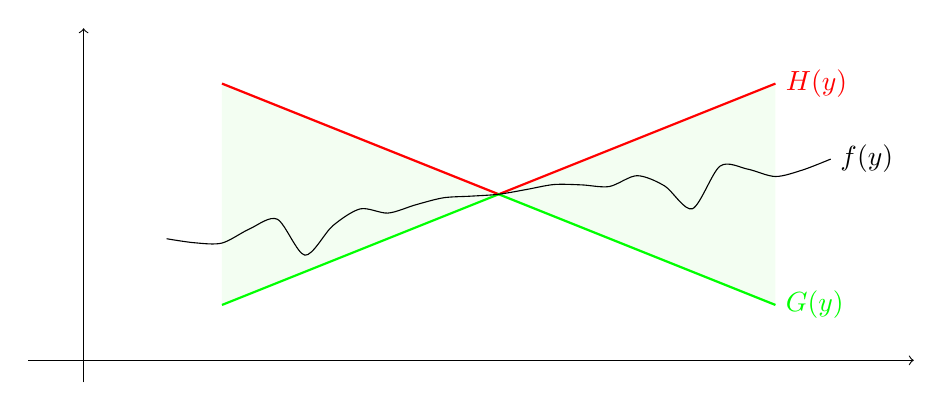
\begin{tikzpicture}[y=40,x=100, declare function={
	wav_sl(\x,\a,\b) = 0.3 * (\x - \a) + \b - 0.1 + 0.1 * cos(20 * pow((\x - \a),2) r) + 0.15 * sin(10 * pow((\x - \a),2) r);
}]
\draw[->] (-0.2, 0) -- (3,0);
\draw[->] (0,-0.2) -- (0,3);

\fill[red!5!green!5] (0.5,2.5) -- (1.5, 1.5) -- (2.5,2.5) -- (2.5,0.5) -- (1.5, 1.5) --  (0.5,0.5);
\draw[thick,-, red] (0.5,2.5) -- (1.5, 1.5) -- (2.5,2.5) node[right] {$H(y)$};
\draw[thick,-, green] (0.5,0.5) -- (1.5, 1.5) -- (2.5,0.5) node[right] {$G(y)$};
\draw[domain=0.3:2.7,smooth,variable=\x,black] plot ({\x},{wav_sl(\x,1.5,1.5)}) node[right] {$f(y)$};
\end{tikzpicture}
\end{figure}

Y lo importante es que lo hace \textbf{en todo el intervalo} que estemos considerando. El mismo cono podemos trasladarlo por la función en todo el intervalo y siempre acotará la función.

En el caso de la raíz cuadrada, vemos que en el 0 vamos a tener una tangente vertical y por lo tanto no vamos a encontrar nunca la constante $L$, ya que tiende a infinito en el cero. Es decir, podemos extraer varias observaciones:

\begin{itemize}
\item Lipschitz implica continua.
\item Lipschitz \textbf{no implica} derivable (p.ej., $\abs{y}$).
\item Derivable \textbf{no implica} Lipschitz global.
\end{itemize}

Parece que podemos encontrar alguna conexión entre Lipschitz y la derivada. Consideramos una $f$ derivable. Entonces 

\[ f(y_1) - f(y_2) = f'(z) (y_1 - y_2) \]

por el teorema del valor medio. Entonces, ese $f'(z)$ sería nuestra constante de Lipschitz $L$. Es decir, la condición de Lipschitz implica acotación de la derivada, que esa $L$ no se va a infinito.

A partir de esta definición podemos llegar a otro nuevo teorema de existencia y unicidad

\begin{theorem}[de existencia y unicidad local] Sea $f(x,y)$ una función continua localmente Lipschitz con respecto a la segunda variable ($y$) en una región $A⊆ℝ^2$ abierta.

Entonces, dado el problema 

\[ \begin{cases}
y'(x) &= f(x,y(x)) \\
y(x_0) &= y_0
\end{cases} \]

con $(x_0, y_0)∈A$, entonces existe una \textbf{única solución local}. Es decir:

\begin{itemize}
\item Existe una constante $α>0$ y una función $y(x)$ que es solución en $[x_0-α, x_0+α]$.
\item Dadas soluciones $y_1$ definida en $[x_0-α_1, x_0+α_1]$, $y_2$ definida en $[x_0-α_2, x_0+α_2]$, ambas son iguales en el intervalo común $[x_0-α_1, x_0+α_1] \cap [x_0-α_2, x_0+α_2]$.
\end{itemize}
\end{theorem}

\begin{proof}
Hay dos formas de llevar a cabo la demostración: o por el teorema de la aplicación contractiva o por el método de iteradas de Picard. Hagamos los dos.

\paragraph{1) T. Aplicación Contractiva} Buscamos demostrar que \[ y(x) = y_0 + \int_{x_0}^x f(s,y(s)) \dif s \] para $x∈[x_0, x_0+h]$.

Trabajaremos en el espacio $X$, el conjunto de funciones $y(x)$ continuas en el intervalo  $[x_0, x_0+h]$ tales que $(x,y(x))∈R_{(x_0, y_0)}\; ∀x∈[x_0, x_0+h]$. 

Definimos la transformación de funciones \[ Ty = y_0 + \int_{x_0}^{x} f(s,y(s)) \dif s \] y buscamos un punto fijo de $T$. Entonces

\[ \abs{Ty(x) - Tz(x)} ≤ \int_{x_0}^{x} \abs{f(s,y(s)) - f(s,z(s))} \dif s \stackrel{\text{Lipschitz}}{≤} \int_{x_0}^x L_R \abs{y(s)-z(s)}\dif s \]

Sabiendo que $\abs{y(s)-z(s)}$ será menor siempre que la norma entre esas dos funciones (ver \ref{defNormaFun}), sustituimos y 

\[ \norm{Ty(x) - Tz(x)}_\infty ≤ L_Rh\norm{y-z}_\infty \]

y por lo tanto será contractivo si $h<\frac{1}{L_R}$.

Sin embargo, el teorema de la aplicación contractiva sólo vale para funciones de un espacio en sí mismo. En este caso, no es seguro que $Ty∈X$. Para poder aplicar el teorema, hay que demostrar que $T$ es una aplicación $\app{T}{X}{X}$. Vamos a ello.

Tenemos que demostrar que si $(x,y(x)) ∈R\; ∀x∈[x_0, x_0+h]$, entonces $(x, Ty(x))∈R\; ∀x∈[x_0, x_0+h]$, o, dicho de otra forma, que $\abs{Ty(x) - y_0}<δ$.  En este caso, vemos que

\[ \abs{Ty(x) - y_0} ≤ \int_{x_0}^x \abs{f(s,y(s))}\dif s \]

Necesitamos que aparezca $y_0$ por alguna razón, así que sumamos y restamos y nos queda 

\[ \abs{Ty(x) - y_0} ≤ \int_{x_0}^x \underbrace{\abs{f(s,y(s))}}_{A} + \underbrace{\abs{f(s,y(s) - f(s,y_0)}}_{B} \dif s \]

Tenemos que $A<C_0$ por ser $f$ continua. Por otro lado, $B<L_R\abs{y-y_0}$ por la condición de Lipschitz, y al estar $y$ en el rectángulo $R$ entonces $B<L_Rδ$. Nos queda entonces 

\[ \abs{Ty(x) - y_0} ≤(C_0 + L_R δ)h \]
y nos bastará tomar $h$ suficientemente pequeño para que se cumpla que $ \abs{Ty(x) - y_0} < δ$, es decir,

\[ h < \frac{δ}{C_0 + L_Rδ} \]

Para finalizar la prueba, nos quedamos con el $h$ mínimo entre este y el que hace que sea contractiva:

\[ h < \min \left\{ \frac{δ}{C_0 + L_Rδ}, \frac{1}{L_R} \right\} \]

\paragraph{2) Iteradas de Picard} Sudo. De hecho

\begin{verbatim}
sudo rual completa esto
\end{verbatim}
\end{proof}

Lo bueno del método de iteradas de Picard es que nos permitirá demostrar un lema adicional de continuidad con respecto a los datos.

\begin{theorem}[de Gronwall] Dada una función 

\[ w(x)≤ h + \int_{x_0}^x k(s)w(s)\dif s \]

con $k$ continua y mayor o igual que cero, entonces 

\[ w(x) ≤ h \exp{\int_{x_0}^xk(s)\dif s} \]
\label{thmGronwall}
\end{theorem}

\begin{proof}

Sea $v(x) = \int_{x_0}^x k(s)w(s)\dif s$. Entonces $v(x_0) = 0$, y  \[ v'(x) = k(x)w(x) \] por el Teorema Fundamental del Cálculo. Sustituyendo de nuevo

\[ v'(x) ≤ k(x) (h + v(x)) = hk(x) + k(x) v(x) \]

Nos queda un sistema

\[ \begin{cases}
v'(x) - k(x)v(x) ≤ hk(x) \\
v(x_0) 
\end{cases} \]

Resolvemos aplicando un factor integrante $μ(x) ≥ 0$. Entonces

\[ μ(x)v'(x) - k(x)μ(x)v(x) ≤ hk(x)μ(x) \] es la ecuación a plantear y nos queda

\begin{gather*}
μ' = -kμ \implies μ(x) = \exp -\int_{x_0}^x k(s) \dif s \\
(μ(x)v(x))' ≤ h k(x) μ(x) \\
(μ(x)v(x))' ≤ -hμ'(x) \\
\int_{x_0}^x (μ(x)v(x))' ≤-h \int_{x_0}^x μ'(s) \dif s 
μ(x)v(x) - \underbrace{μ(x_0) v(x_0)}_0 ≤ -h (μ(x) - \underbrace{μ(x_0)}_1)
\end{gather*}

En total, nos queda

\begin{gather*}
\exp\left(-\int_{x_0}^x k(s)\dif s\right) v(x) ≤ -h \left(\exp\left(-\int_{x_0}^x k(s)\dif s\right) - 1\right) \\
w(x) - h ≤ v(x) ≤ h \left(\exp\left(-\int_{x_0}^x k(s)\dif s\right) - 1\right) \\
w(x) ≤ h \exp\left(-\int_{x_0}^x k(s)\dif s\right) 
\end{gather*}

En un caso más general, si tengo que \[ w(x) ≤ h(x) + \int_{x_0}^x k(s)w(s)\dif s \] con $k$ continua y mayor o igual que cero, llegaríamos a la conclusión haciendo cuentas análogas de que

\[ w(x) ≤ h(x) + \int_{x_0}^x h(s) k(s) e^{\int_{x_0}^xk(t)\dif t} \dif s \]

\end{proof}

Con este lema, podemos construir otro de continuidad respecto de los datos.

\begin{theorem}[Continuidad respecto de los datos]\label{thmContDatos}

Dados dos problemas

\[ \begin{cases}
y'(x) &= f(x,y(x)) \\
y(x_0) &= y_0
\end{cases}, \begin{cases}
z'(x) &= f(x,z(x)) \\
z(x_0) &= z_0
\end{cases} \] con $f$ función Lipschitz, entonces 

\[ \abs{y(x)-z(x)} ≤ \abs{y_0-z_0} M \] con $M∈ℝ$.

Dicho de otra forma, datos próximos nos dan soluciones próximas.
\end{theorem}

\begin{proof}

Dados dos problemas

\[ \begin{cases}
y'(x) &= f(x,y(x)) \\
y(x_0) &= y_0
\end{cases}, \begin{cases}
z'(x) &= f(x,z(x)) \\
z(x_0) &= z_0
\end{cases} \]

tenemos que

\begin{gather*}
y(x) = y_0 + \int_{x_0}^{x} f(s,y(s)) \dif s \\
z(x) = z_0 + \int_{x_0}^{x} f(s,z(s)) \dif s 
\end{gather*}

Entonces, si restamos y tomamos valores absolutos,

\begin{multline*}
 \abs{y(x) - z(x)} ≤ \abs{y_0-z_0} + \int_{x_0}^x \abs{f(s,y(s)) - f(s,z(s))} \dif s \\ \stackrel{\text{Lipschitz}}{≤}  \abs{y_0-z_0} + \int_{x_0}^x L_R\abs{y(s)-z(s)} \dif s \end{multline*}

Podemos aplicar el Lema de Gronwall a esta ecuación:

\[ \underbrace{\abs{y(x) - z(x)}}_{w(x)} ≤ \underbrace{\abs{y_0-z_0}}_{C} + \int_{x_0}^{x} \underbrace{L_R}_{k(s)} \underbrace{\abs{y(s)-z(s)}}_{w(x)} \dif s \]

y entonces tenemos que 

\[ \abs{y(x)-z(x)} ≤ \abs{y_0-z_0}e^{\int_{x_0}^{x}L_R\dif S} = \abs{y_0-z_0} M \]

donde $M$ es una constante, así que tenemos la continuidad.
\end{proof}

\subsection{Ejercicios}

\begin{example} Analiza la convergencia puntual y uniforme de las siguientes sucesiones de funciones.

\begin{enumerate}
\item $f_n(x) = x^n -x^{n+1}$ en $[0,1]$.
\item $f_n(x) = \frac{e^x}{x^n}$ en $(1,∞)$.
\item $f_n(x) = x^n - x^{2n}$ en $[0,1]$.
\item $f_n(x) = n \left(\sqrt{x + \frac{1}{n}} - \sqrt{x}\right)$ en $x > 0$.
\item $f_n(x) = \sin\left(\frac{x}{n}\right)$ con $x∈ℝ$.
\end{enumerate}

\paragraph{$f_n(x) = x^n -x^{n+1}$} Buscamos primero la convergencia puntual, y tenemos que 

\[ \lim_{n\to ∞} x^n-x^{n+1} = 0 \] por lo que converge puntualmente.

Estudiamos ahora la convergencia uniforme con el límite

\[ \lim_{n\to ∞} \max_{x∈[0,1]} \abs{f_n(x) - 0} = \lim_{n\to ∞} \max_{x∈[0,1]} x^n - x^{n+1} \]

Para hallar el máximo, derivamos e igualamos a cero:

\[ nx^{n-1} - (n+1){x^{n-1}} = x^{n-1}(n-(n+1)x) = 0 \] y nos queda 

\[ \lim_{n\to ∞} \max_{x∈[0,1]} f_n(x) = f_n\left(\frac{n}{n+1}\right) = \underbrace{\frac{1}{\left(1+\frac{1}{n}\right)^n}}_{\convs \frac{1}{e}} \cdot \underbrace{\frac{1}{n+1}}_{\convs 0} = 0 \] y por lo tanto hay convergencia uniforme.

\paragraph{$f_n(x) = \frac{e^x}{x^n}$} Puntualmente y con $x>1$

\[ \lim_{n\to ∞} x^{-n} e^x = 0 \]

Estudiamos la convergencia uniforme

\[ \lim_{n\to ∞} \sup_{x>1} \abs{f_n(x)} = \lim_{n\to ∞} \sup_{x>1} x^{-n} e^x \]

Derivamos e igualamos a cero

\[ e^xx^{-n-1}(x-n) = 0 \iff x=n \]

y evaluando

\[ \lim_{n\to ∞} \eval{f_n(x)}_{x=n} = \lim_{n\to ∞} \left(\frac{e}{n}\right)^n = 0 \]

Ojo, porque en este caso no tenemos convergencia uniforme. No hemos demostrado que en $x=n$ haya un máximo: de hecho, es un mínimo. También tendríamos que tener cuidado con el supremo y no el máximo, ya que estamos en un conjunto no acotado.

\paragraph{$f_n(x) = x^n - x^{2n}$} Convergencia puntual. Cero. Uniforme: otra vez lo del límite, puede poner máximo.\footnote{Esta mierda de ejercicio que estoy copiando está patrocinado por la falta de sueño por culpa de redes.} Deriva. Saca algo. Es un máximo. Evalúa, distinto de cero, no hay convergencia uniforme.

\paragraph{$f_n(x) = n \left(\sqrt{x + \frac{1}{n}} - \sqrt{x}\right)$} Hay que hacer el conjugado... se va a algún sitio y $\frac{1}{2\sqrt{x}} = f(x)$ es el límite puntual. Vamos a la uniforme y miramos si converge al límite puntual

\[ \lim_{n\to ∞} \sup_{x∈(0,∞)} \abs{f_n(x) - f(x)} \]

pero ese uno entre dos raíz de equis se va a menos infinito, y como tenemos hun balor havzolutoh me ahorro las dos caras de cuentas de derivadas de Azorero. Pero dice que no, que comprobemos en $(1/2, + ∞)$.

\paragraph{ $f_n(x) = \sin\left(\frac{x}{n}\right)$} Parece que sí hay convergencia puntual. No hay uniforme en todo $ℝ$ ya que habrá algún valor en el que el seno valga uno. Sin embargo, en un intervalo acotado sí habrá convergencia uniforme.
\end{example}


\begin{example} Determinar para qué valores de $α≥0$ se satisface una condición de Lipschitz con respecto de $y$ siendo 

\[ f(x) = \abs{y}^α \].

Es trivial ver que para $α=0,1$, se cumple. Para valores mayores que 1, la derivada estará acotada si estudiamos la condición en intervalos acotados. Si $α<1$, tendremos problemas en el 0.

La filosofía es que raíces malas en el 0, potencias malas en el infinito.

Supongamos $y>0$, entonces $f'(y) = α y^{α-1}$. Para $α>1$, 

\[ \abs{f(y_1)-f(y_2)} \stackrel{TVM}{=} \abs{f'(z)} \abs{y_1-y_2} = αz^{α-1} \abs{y_1-y_2} \stackrel{?}{<} L \abs{y_1-y_2} \]

y entonces debe ser $αz^{α-1}<L$, es decir, tenemos que tener una cuota superior para $y_2$.
\end{example}


\subsection{Diferenciabilidad con respecto a los datos}

Hasta ahora hemos estado viendo problemas de la forma

\[ \begin{cases}
y' = f(x,y) \\
y(x_0) = t
\end{cases} \]. 

En realidad, al resolver, obtenemos funciones $y(x,t)$, una familia de soluciones que dependen del valor inicial de $t$. 

Sabemos que si $f(x,y)$ es continua y localmente Lipschitz en un abierto $A⊆ℝ^2$ con $(x_0,t)∈A$, entonces tenemos existencia y unicidad local.

Por otro lado, también demostramos un resultado de continuidad con respecto a los datos. Es decir, $y(x,t)$ es continua con respecto a $t$ (ver lema \ref{thmContDatos}). 

El paso siguiente es ver qué ocurre cuando $f$ es algo \textit{mejor} que Lipschitz: $y(x,t)$ será también \textit{mejor}. Veamos el teorema:

\begin{theorem}[Diferenciabilidad respecto a los datos] Si $f$ es una función continua en $x$ y además $C^1$ con respecto a la segunda variable, entonces la solución $y(x,t)$ es derivable respecto de $t$.
\end{theorem}

\begin{proof} Fijamos $t$, y estudiamos el límite que representa la derivada

\[ \lim_{h\to 0} \frac{y(x,t+h) - y(x,t)}{h} = \lim_{h\to 0} P_h(x) \]

Dicho de otra forma,

\[ P_h(x) = \frac{1}{h}\left((t+h) + \int_{x_0}^x f(s, y(s, t+h)\dif s - t - \int_{x_0}^x f(s, y(s, t)\dif s\right) \] 
que no es más que la reformulación usando la forma integral de $y$. Si seguimos operando

\[ P_h(x) = 1 + \int_{x_0}^x\frac{1}{h}\left(f(s, y(s,t+h)) - f(s,y(s,t+h))\right)\dif s \]

Si aplicamos el teorema del valor medio

\[ P_h(x) = 1 + \int_{x_0^x} \underbrace{\pd{f}{y}(s,z(s,h))}_{F}\underbrace{\frac{1}{h} (y(s,t+h) - y(s,t))}_{P_h(x)} \dif s \]

con $z(s,h)$ un valor intermedio entre $y(s,t)$ e $y(s,t+h)$, que tiende a $y(s,t)$ cuando $h\to 0$. Llamamos $F$ a la derivada parcial para simplificar, y además vemos que nos vuelve a salir $P_h$. Reescribimos

\[ P = 1 + \int_{x_0}^{x} FP \dif s \]
y vemos que estamos antes la formulación integral del siguiente problema

\[ \begin{cases}
P' = FP \\
P(x_0) = 1
\end{cases} \implies P = e^{\int_{x_0}^x F\dif s} \]

Calculamos ahora el límite de $P_h$ cuando $h\to 0$. El punto delicado es cómo pasar el límite de fuera de la integral a dentro. Asumiendo que se puede hacer sin problemas, quedaría

\[ \lim_{h\to 0} P_h(x) = \exp{\int_{x_0}^x \pd{f}{y}(s,y(s,t)) \dif s} = \pd{y}{t} \]

Para poder pasar el límite, tenemos que tener convergencia uniforme. Como estamos trabajando en un conjunto compacto con una función continua, la función es uniformemente continua , tendremos esa convergencia y podremos pasar el límite dentro.

\end{proof}

\subsection{Resultados de prolongabilidad}

Queremos explorar hasta dónde llegan las soluciones que obtenemos y el tipo de desastres que podemos encontrar. Tenemos el problema de siempre,

\[ \begin{cases}
y' = f(x,y) \\
y(x_0) = t
\end{cases} \], con $f(x,y)$ es continua y localmente Lipschitz en un abierto $A⊆ℝ^2$ con $(x_0,t)∈A$, entonces tenemos existencia y unicidad local.

Sabemos varias cosas:

\begin{itemize}
\item \textbf{Existencia local} $∃α>0, y(x)$ solución definida en $[x_0,x_0 + α]$.
\item \textbf{Unicidad} Si tenemos dos soluciones $y_1,y_2$ definidas en los intervalos $[x_0, x_0 + α_{1/2}]$ respectivamente, entonces ambas son iguales en el intervalo $[x_0, x_0 + \min \{α_1,α_2\}]$.
\end{itemize}

La pregunta es, ¿hay una solución maximal, que no se pueda extender más? Consideremos el conjunto

\[ S= \{ α∈ℝ \st ∃ y(x) \text{ solución en } [x_0,x_0+α] \} \]

Buscamos $α_{max} = \sup S$, que nos dará el intervalo maximal $[x_0, x_0 + α_{max})$. Es importante tener en cuenta que el intervalo está abierto por la derecha. 

Lo primero que tenemos que considerar es que en el intervalo maximal no puede haber dos soluciones distintas que arranquen del mismo punto. 

Si nos salimos fuera del conjunto $A$ en el que la función es Lipschitz, podemos tener un desastre. ¿Qué puede ocurrir dentro?

Podemos tener una solución que \textit{se pare antes}, que oscile infinitamente, que llegue al borde o que explote.\footnote{Dibujitos}

El teorema nos dice que las primeras dos cosas no pueden ocurrir, y que las dos segundas sí. Esta cosa tan vaga la formalizamos viendo que toda solución se escapa de cualquier conjunto compacto estrictamente contenido en $A$ y que contenga al dato inicial. 

\begin{theorem}
Consideramos el problema
\[ \begin{cases}
y' &=f(x,y) \\ 
y(x_0)&=y_0
\end{cases} \]
con $f$ continua y localmente Lipschitz respecto de $y$ en un abierto $A\subset \real^2$ con $(x_0,y_0)\in A$. 

Entonces para cualquier compacto K con $(x_0,y_0)\in K\subset A$, podemos encontrar $x^{\ast}\in[x_0,x_0+\alpha_{max})$ tal que $(x^{\ast},y(x^{\ast}))\in A-K$.


\end{theorem}

\begin{proof}
Llamamos $S\equiv \{\alpha\in\real \st \text{ la solución y(x) está definida en } [x_0,x_0+\alpha] \}$ y $\alpha_{max} = sup(s)$.

$\forall n>0$ podemos encontrar $x_n \in \left(x_0 + \alpha_{max} - \frac{1}{n},x_0+\alpha_{max}\right)$ tal que $s_n\in S$, donde 

Entonces podremos construir una sucesión $x_n$ creciente de Cauchy cuyo límite es $x_0+\alpha_{max}$ en $x_0 + \alpha_{max}$ tal que y esté definida en todos los $x_n$.

Vamos a demostrarlo por \textbf{reducción al absurdo:}

Supongamos $(x,y(x))\subset K, \forall x\in[x_0,x_0+\alpha_{max}]$.

En particular $\{(x_n,y(x_n))\}\subset K$,


Entonces queremos ver que $| y(x_n) - y(x_m)|$ para comprobar si es convergente y si tiene límite utilizando el criterio de Cauchy.

Poniendolo en notación integral:

\[| y(x_n) - y(x_m)| \underset{m>n}{=} y_0 + \int_{x_n}^{x_m} f(s,y(s))ds \leq M |x_m-x_n| \]

\paragraph{Conclusión:}
Por ser $\{X_n\}$ convergente, entonces $\{y(x_n)\}$ es de Cauchy y por tanto tiene límite, que vamos a llamar $y^{\ast}$ .

Como K es compacto, entonces $y^{\ast}\in K$. (por ser límite de la sucesión).

¿Podemos definir $y(x_0+\alpha_{max} = y^{\ast})$? 
\textbf{Respuesta:} Todavía no. Si tuvieramos una solución que oscile al acercarse a la frontera, el límite dependería de la sucesión que eligiéramos. Necesitamos demostrar que $y^{\ast}$ no depende de la sucesión $\{x_n\}$ de puntos de la curva que hayamos elegido.

Para ello: sea $\{z_n\}$ ptra sucesión con $z_n$ que se aproxima a $x_0+\alpha_{max}$. ¿Qué pasa con $|y(x_n) - y(z_n)| \to 0$? 


\[|y(x_n) - y(z_n)| = \int_{x_n}^{z_n} f(s,y(s))ds \underset{\begin{array}{c}(x,y(x))\in K \subset A\\\text{ f continua }\end{array}}{\leq}M |z_n - x_n| \to 0 \implies (*) \]
\[(*) \implies \exists!y^{\ast} \st y^{\ast} = \lim_{x\to (x_0+\alpha_{max})^{-}} y(x) \text{ para cualquier sucesión con límite } x_0+\alpha_{max}\]


Estudiamos este problema:
\[\begin{array}{cc}
y' &= f(x,y)\\
y(x_0+\alpha_{max} &= y^{\ast})
\end{array}\]
Por ser Lipschitz tenemos el teorema de existencia y unicidad local (refrencia) entonces tendríamos una solución que sobrepase el punto $x_0+\alpha_{max}$ contradiciendo la hipótesis.

\end{proof}

Algunas estimaciones del intervalo maximal. 

Vamos a considerar $A \equiv (x,b)×ℝ$, es decir, una banda vertical en $\real^2$.

\paragraph{Caso 1}
Supongamos que la $f(x,y)\leq C,\forall (x,y)\in A$ (está acotada). Además suponemos (como siempre) que $f$ es continua y localmente Lipschitz.

Tenemos un $(x_0,y_0)$ y queremos comprobar si la solución llega al extremo (o por el contrario tiene una asíntota).

Sea la solución: $\displaystyle y(x) = y_0 + \int_{x_0}^{x} f(s,y(s))ds\, x\int [x_0,x_0+\alpha_{max})\subset [x_0,b)$.

\[y(x) - y_0| \leq \int_{x_0}^x |f(s,y(s))|ds \leq C |x-x_0|\]

\[y(x) - y_0|\leq C |x-x_0| \implies y_0 - C(x-x_0) \leq y(x) \leq y_0 + C(x - x_0)\] es decir, está controlada por las rectas $y_0 \pm C(x-x_0)$ evitando así cualquier asíntota vertical. Además, el teorema anterior nos dice que la solución se sale del conjunto compacto, con lo que el intervalo maximal llega hasta b.

\textbf{Lado derecho acotado implica solución global en (a,b)}

\paragraph{Caso 2} Supongamos $|f(x,y)|\leq A(x)|y| + B(x);\, A,B\ge 0$ continuas en (a,b)

Trabajando con notación integral:
\[|y(x)| \leq  |y_0| + \int_{x_0}^x | A(s)|y(s)| + B(s)|ds = \underbrace{|y_0| + \int_{x_0}^x B(s)ds}_{C} + \int_{x_0}^x A(s)|y(s)|ds \]
Esta es una desigualdad que nos permite aplicar el lema de Gronwall.

Entonces $|y(x)| \leq C \exp{\int_{x_0}^{b^{\ast}} A(s)ds }$.

Donde $b^{\ast}$ es un punto arbitrario para acotar la solución con un valor que no dependa de $x$.

\textbf{El intervalo maximal $\equiv (a,b)$}


\paragraph{Ejemplo:} 
\[\begin{array}{cc}
y'&=y^2\\
y(0)&=1
\end{array}\]

\[\frac{y'}{y^2} = 1 ; \int_0^x \frac{y'/s(ds)}{(y(s))^2} = \int_0^x 1ds = x \implies ... \implies y(x) = \frac{1}{1-x}\]
Aquí el intervalo maximal hacia la derecha es $[0,1)$.

Sin embargo, el lado derecho ($y^2$) es localmente Lipschizt en todo $\real^2$.

Vamos a demostrarlo para recordar: Siendo una función derivable, aplicamos que si la derivada está acotada, entonces la primitiva el Lipstchizt. 

Como $2y$ es localmente acotada, entonces $y^2$ es localmente Lipschitz.

Vamos a definir un compacto $K = [0,R]×[1,1+h]$ y por el teorema anterior sabemos que la solución se escapa del compacto. Ahora vamos a ver si por arriba o por la derecha (para ver hasta donde llega el intervalo maximal).

\[0\leq y' \leq (1+h)^2\]
Integrando, (con alguna cuenta intermedia) obtenemos:
\[1\leq y (x) = 1 + (1+h)^2 x\]

Es decir, la solución está acotada por 2 rectras, $y=1$ por abajo y $1 + (1+h)^2 x$ por arriba (hasta el corte con el borde superior del compacto, que llamamos $R(h)$).

Lo único que podemos decir es que la solución no ha \textit{explotado} antes de $R(h)$.

Vamos a calcular (creo que por diversión) cuánto vale $R(h)$.
\[(1+h) = (1+h)^2x+1\]
\[R(h) = \frac{h}{(1+h)^2}\]


No era por diversión. Si tenemos $h\to \infty$ ó $h=0 \implies R(h) \to 0$. Esto nos da un máximo: $h=1; R(1)=\frac{1}{4}$.

\textbf{Conclusión} el intervalo de existencia contiene a $\left[0,\frac{1}{4}\right]$.

El dibujo de los triángulos te lo dejo a ti Rual xD

Haciendo el apaño de los triángulos llegamos a un intervalo $\left[0,\frac{1}{2}\right]$

Vamos a ver un ejemplo más sencillo por el que tendríamos que haber empezado (tal vez) q estoy muy cansado como para copiar........

\footnote{Quince primeros minutos de clase faltan aquí}

\begin{example}
Veamos el problema \[ \begin{cases} y' &= y^{2/3} \\ y(0) &= 0 \end{cases} \]

No podemos aplicar directamente el teorema de existencia y unicidad: la derivada no está acotada alrededor de 0 y por lo tanto no es localmente Lipschitz en ese punto. Si nos dijeran que $y(0) = ε ≠ 0$ sí sería localmente Lipschitz en un entorno pequeño del punto.

Como no podemos aplicar el teorema, tenemos que estudiar el caso más detenidamente. En primer lugar, vemos que $y\equiv 0$ es solución. También podemos resolver como una ecuación de variables separadas:

\[ \int_0^x \frac{y(s)}{y^{2/3}(s)} \dif s = \int_0^x \dif s = x \] sobre la que podemos hacer un cambio de variables $y(s) = t$, $y'(s) \dif s = \dif t$ y entonces

\[ \int_{y(0)}^{y(x)} \frac{\dif t}{t^{2/3}} = \eval{t^{1/3}{\frac{1}{3}}}_{t=y(0)=0}^{y(x)} = 3y^{1/3}(x) 
\] 
y por lo tanto \[ y(x) = \left(\frac{x}{3}\right)^3 \] es otra solución.

¿Hay alguna más? Efectivamente, de hecho podemos combinar las dos:

\[ y(x) = \begin{cases}
0 & x ≤ 0 \\
\left(\frac{x}{3}\right)^3 & x > 0
\end{cases}\quad \text{\'o} \quad y(x) = \begin{cases}
\left(\frac{x}{3}\right)^3 & x ≤ 0 \\
0 & x ≤ 0\end{cases} \]

E incluso podemos conseguir infinitas soluciones combinando "desplazamientos", como por ejemplo el de la figura \ref{imgInfSoluciones}.
\end{example}

\begin{figure}[hbtp]
\centering
\begin{tikzpicture}
\draw[->] (-3,0) -- (3,0);
\draw[->] (0,-3) -- (0,3);

\draw[thick,domain=-2.8:1,smooth,variable=\x,blue!80] plot ({\x}, {0});
\draw[thick,domain=1:2.8,smooth,variable=\x,blue!80] plot ({\x}, {(\x-1)*(\x-1)*(\x-1)/3});
\end{tikzpicture}
\label{imgInfSoluciones}
\caption{Una solución posible trasladando otra con dato inicial $y(1) = 0$}
\end{figure}


Sin embargo, no tiene por qué ocurrir siempre que se nos descuadre todo al no poder aplicar la condición de Lipschitz. Veamos otro ejemplo

\begin{example}
 \[ \begin{cases} y' &= (y-x)^{2/3} \\ y(x_0) &= y_0 \end{cases} \]
 
 En este caso los problemas aparecen cuando $y=x$. Es decir, que podemos aplicar el teorema de existencia y unicidad local cuando $y_0 ≠ x_0$. 
 
 Supongamos, por poner las cosas interesantes, que $y(1) = 1$. Hay que estudiar este caso directamente.
 
 Podemos resolverlo a través del teorema de la función implícita. Sea $w(x) = y - x$. Haciendo las sustituciones
 
 \begin{gather*}
 y(x) = w(x) + x \\
 y' = w' + 1
 \end{gather*} 
 
 convertimos el problema en 
 
 \[ \begin{cases}
 w'+1 = w^{2/3} \\
 w(1)  = 0
 \end{cases} \]
 
 Resolviendo como ecuación de variables separadas de la misma forma que en el anterior ejemplo, llegamos a la integral
 
 \[ \int_{0}^{w(x)}  \frac{\dif t}{t^{2/3} - 1} \]
 
 Y ahí está la solución, si pudiésemos resolver explícitamente la integral y despejar $w$. Pero podemos usar el teorema de la función implícita. Tenemos una función $F$ definida como
 
 \[ F(x,w) = (x-1) - \int_{0}^{w(x)}  \frac{\dif t}{t^{2/3} - 1} 
 \] 
 con $F(1,0) = 0$. ¿Podemos despejar $w(x)$? Para saberlo necesitamos comprobar que la derivada es distinta de cero:
 
 \[ \pd{F}{w} = - \eval{\frac{1}{w^{2/3} - 1}}_{(x,w) = (1,0)} = 1 ≠ 0 \] y por lo tanto el TFI nos dice que existe $w(x)$ despejable a partir de $F$ y que además es única.
\end{example}

En resumidas cuentas, cuando no se cumplen las hipótesis del teorema puede pasar cualquier cosa. Veamos otro ejemplo bastante artificial pero interesante.

\begin{example}
\[ \begin{cases}
y' &= \frac{\sqrt{1-y^2}}{1+x^2} \\
y(0) = \frac{1}{2}
\end{cases} \]

La ecuación nos restringe $y$ al intervalo $[-1,1]$ para que la raíz cuadrada esté definida. Y de hecho, en esos dos extremos del intervalo la derivada será cero así que tendremos un problema. Por otra parte, $y\equiv \pm 1$ son soluciones de la ecuación (no del problema entero).

La solución es

\[ y(x) = \sin \left(\frac{1}{1-x} - 1 + \frac{π}{4}\right) 
\]
que no es más que una traslación de la función $\sin\frac{1}{1-x}$, cuya gráfica se ve en la figura \ref{imgSenoOsc}. En $1$ tenemos un montón de oscilaciones, por lo tanto el intervalo maximal de la solución será $[0, 1)$.
\end{example}

\begin{figure}[hbtp]
\centering
\includegraphics[width=0.8\textwidth]{img/SenoOscilaciones.png}
\caption{$y(x) = \sin\frac{1}{1-x}$}
\label{imgSenoOsc}
\end{figure}

\begin{example} 

\[ \begin{cases}
y' = \dfrac{x^2 + 4y^2 + xy}{1 + x^2 + y^2} \\
y(x_0) = y_0
\end{cases} \]

Se verifica condición de Lipschitz local y por lo tanto tenemos existencia y unicidad local para cualquier punto $(x_0,y_0)$. ¿Hasta dónde llega la solución?

Podemos aplicar uno de los tres casos que hemos visto. Los dos polinomios son del mismo orden, por lo tanto el lado derecho estará acotado y tendremos el primer caso, de tal forma que tenemos existencia global.

Vamos a demostrar mejor la existencia de esa cota.

\begin{multline*}
 \dfrac{x^2 + 4y^2 + xy}{1 + x^2 + y^2} ≤ \dfrac{x^2 + y^2 + 3y^2 + \abs{xy}}{1 + x^2 + y^2} ≤ \dfrac{1 + x^2 + y^2 + 3 y^2 + xy}{1 + x^2 + y^2} =\\ =
  1 + \frac{3y^2 + \abs{xy}}{1+x^2+y^2} ≤ 1 + \frac{3(1+x^2+y^2) + \abs{xy}}{1+x^2+y^2} = 4 + \frac{\abs{xy}}{1+x^2+y^2} \end{multline*}

Por último, viendo que $0≤(x-y)^2 = y^2+x^2 - 2xy \implies \dfrac{x^2+y^2}{2} ≥ xy$ nos queda que 

\[ 
	4 + \frac{\abs{xy}}{1+x^2+y^2} ≤ 4 + \frac{x^2+y^2}{2(1+x^2+y^2)} ≤ 4 + \frac{1 x^2+y^2}{2(1+x^2+y^2)} = 4 + \frac{1}{2} 
\]
y, efectivamente, nos queda una cota.


\end{example}

En muchos casos nos encontraremos cálculos complicados, y en estos casos podemos usar argumentos de comparación con problemas más simples. Veamos cómo hacerlo.

\begin{example}
\[ \begin{cases} 
y' = y^2 +x^2 \\
y(0) = 1
\end{cases} \]

A pesar de la sencillez de la ecuación, resolverla será difícil. Podemos explorar ecuaciones similares. Por ejemplo, viendo que el dato inicial nos lo dan en $x=0$, podemos pensar que la ecuación deberá parecerse mucho a 

\[ \begin{cases} 
z' = z^2 \\ 
z(0) = 1
\end{cases} \].


\begin{wrapfigure}{r}{0.4\textwidth}
\centering
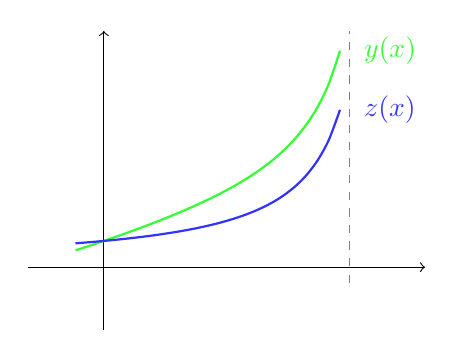
\begin{tikzpicture}[xscale=1.2]
\draw[->] (-0.8,0) -- (3.4,0);
\draw[->] (0,-0.8) -- (0,3);

\draw[thick,domain=-0.3:2.5,smooth,variable=\x,green!80] plot ({\x}, {1/(3-\x) + 0.3*\x})  node[right,xshift=5pt] {$y(x)$};
\draw[thick,domain=-0.3:2.5,smooth,variable=\x,blue!80] plot ({\x}, {1/(3-\x)}) node[right,xshift=5pt] {$z(x)$};
\draw[dashed, gray] (2.6,-0.2) -- (2.6, 3);
\end{tikzpicture}
\caption{Gráfica de $y(x)$ y $z(x)$.}
\label{imgGraficaAprox}
\end{wrapfigure}

Vemos que la gráfica de $z$ se mantendrá por debajo todo el tiempo, ya que $z' < y'$ en todo caso (ver figura \ref{imgGraficaAprox}). Como la solución del segundo problema es $z(t) = \dfrac{1}{1-t}$, $y$ también tendrá una asíntota vertical en $t=1$ o incluso antes. Por lo tanto, el intervalo maximal a la derecha para $y(t)$ está contenido en $(0,1)$.

También podemos llegar al mismo resultado de otra forma, trabajando con desigualdades. Sabiendo que $y$ es siempre mayor que cero, podemos decir

\[ y'= y^2+x^2 ≥ y^2 \implies \frac{y'}{y^2} ≥ 1 \]

Integrando
\[
 \int_0^x \frac{y'(s)}{y^2(s)}\dif s ≥ \int_0^x \dif s = x
\] 
y haciendo cambio de variable $y(s) = t$, $y'(s)\dif s = \dif t$
\[ 
\int_1^{y(x)}\frac{\dif t}{t^2} = \eval{\frac{-1}{t}}_{t=1}^{y(x)} = 1 - \frac{1}{y(x)}
\].

Con esto nos quedaría la siguiente desigualdad.

\[ y(x) ≥ \frac{1}{1-x} \].

También podemos hacer una segunda estimación. Aplicando que el intervalo maximal de nuestra solución es como  mucho $(0,1)$, vemos que
\[ 
y' = y^2 + x^2 ≤ y^2 + 1
\]
lo que nos daría una nueva estimación

\[ y(x) ≤ \tan\left(x + \frac{π}{4}\right) \].

Juntando todos los resultados, tendríamos una estimación como la de la figura \ref{imgEstRegion}.

\end{example}


\begin{figure}[hbtp]
\centering
\begin{tikzpicture}[xscale=1.5, yscale=1.2]
\draw[->] (-0.8,0) -- (3.4,0);
\draw[->] (0,-0.8) -- (0,3);

\draw[thick,domain=-0.3:0.6,smooth,variable=\x,green!80] plot ({\x}, {tan((\x + pi/4) r) / 2}) node[right,xshift=5pt] {$\tan\left(x + \dfrac{π}{4}\right)$};
\draw[thick,domain=-0.3:2.5,smooth,variable=\x,blue!80] plot ({\x}, {1/(3-\x)}) node[right,xshift=5pt] {$\dfrac{1}{1-x}$};
\draw[dashed, gray] (2.6,-0.1) -- (2.6, 3);
\draw[dashed, gray] (0.65,-0.1) -- (0.65, 3);
\node[label=below:{$\dfrac{π}{4}$}] at (0.65,0) {};
\node[label=below:{$1$}] at (2.6,0) {};

\end{tikzpicture}
\caption{La función real $y(x)$ estará entre las dos funciones que hemos estimado..}
\label{imgEstRegion}
\end{figure}

\paragraph{Método de las poligonales de Euler y funciones no-Lipschitz} Consideremos el ejemplo anterior de $y'=y^{2/3}$. Si aplicamos el método de las poligonales de Euler, no encontraríamos ninguna otra solución que no fuese la constante $y\equiv 0$. Sin embargo, si tomamos un punto inicial $y(0) = ε$ la solución sí crecerá. Por lo tanto, si no tenemos un teorema que nos garantice unicidad tendremos que estudiar qué ocurre alrededor de ese punto para comprobar que no nos dejamos ecuaciones.

Sigamos con más ejemplos.


\begin{figure}[hbtp]
\centering
\begin{tikzpicture}[xscale=2,yscale=1.4]

\draw[->] (-0.8,0) -- (3,0);
\draw[->] (0,-0.8) -- (0,2);

\draw[gray,-,fill=orange!10] (0,0) rectangle (2,1);
\draw[pattern=horizontal lines, pattern color=red!70!orange] (0,0) -- (0.86,1) -- (2,1) -- (2,0) -- (0,0);
\path[name path=hl] (0,1) -- (2,1);
\draw[name path=fn, very thick,-] (-0.5,-0.6) -- (1.5,1.8) node[right] {$(h^4+r)x$};

\path [name intersections={of=hl and fn,by=E}];
\node (I) [above=0.5 of E] {};
\node (IO) [below=1 of E] {};
\draw[dashed] (I) -- (IO);
\node[vnlin,label=below:{$R(h)$},anchor=north] at (IO) {};

\node[anchor=north west,orange!80!black] at (0,1) {$K$};
\node[hnlin,gray,label=left:{$h$}] at (0,1) {};
\node[vnlin,gray,label=below:{$R$}] at (2,0) {};
\end{tikzpicture}
\caption{Representación del conjunto $K$, donde la zona rayada es donde encontraremos la solución.}
\label{figConjuntoK}
\end{figure}

\begin{example}
\[ \begin{cases}
y' = y^4 + r \\
y(0) = 0
\end{cases}
\] 
con $r>0$. La ecuación verifica una condición de Lipschitz local. A primera vista vemos que $y'>0$ y por lo tanto $y≥0$.

Consideramos el conjunto $K$, un rectángulo de altura $h$ y anchura $R$ (figura \ref{figConjuntoK}). Podemos hacer una estimación y operar

\begin{gather*}
0 ≤ y^4 + r ≤ h^4 + r \\
0 ≤ y' ≤ h^4 + r \\
0 ≤ y(x) ≤ (h^4+r)x \quad ∀(x,y) ∈ K
\end{gather*}

Por lo tanto, la solución tendrá un intervalo maximal a la derecha $[0,b)$, donde $b$ será mayor o igual a $R(h)$, que es la intersección de la recta $(h^4+r)x$ con $y=h$, es decir

\[ R(h) = \frac{h}{h^4+r} \]

Queremos hallar el $R(h)$ óptimo, así que derivando y operando obtenemos que

\[ b ≥ R(h_{max}) = \left(\frac{r}{3}\right)^{-3/4} \frac{1}{4} \]

Tomemos ahora la indicación del problema. Suponemos que $b>r^{-3/4}$. ¿Qué estimación podemos obtener a partir de esto? 
\end{example}



\begin{example}[Problema 16]
Tenemos 

\[ \begin{cases}
y' = \frac{y}{1+x^2} + e^{-y^2} \\
y(0) = 10
\end{cases},\quad 
\begin{cases}
z' = \frac{z}{1+x^2} \\
z(0) = 10
\end{cases} \]

Queremos demostrar que $0< y(x) - z(x) ≤ e^{-100} (e^x-1)$.

En el caso de la primera ecuación, vemos que $y'≥0$, así que $y(x) ≥ 10\,∀x ≥ 0$. Además, $f(x,y)$ es continua en $ℝ^2$. Para comprobar la condición de Lipschitz, acotamos

\[ \abs{\pd{f}{y}} = \abs{\frac{1}{1+x^2}+e^{y^2}(-2y)} ≤ \frac{1}{1+x^2} + 2\abs{y} e^{-y^2} ≤ 1+2\abs{y} 
\] 
y tenemos condición de Lipschitz local, por lo que tenemos existencia y unicidad local. Además, también podemos acotar el lado derecho de la ecuación por un término lineal:

\[ \abs{f(x,y)} ≤ \abs{\frac{y}{1+x^2} + e^{-y^2}} ≤ \frac{\abs{y}}{1+x^2} + e^{-y^2} ≤ \abs{y} + 1 
\]
lo que, junto con el segundo teorema de prolongabilidad, tenemos existencia en $[a,b]$  $∀a,b$.

Pero además, podríamos haber logrado una cota mejor para $2\abs{y} e^{-y^2}$. Sabiendo que es una función continua y que tiende a 0 cuando $y\to \infty$, podemos decir que existe un máximo $C$. Acotando esa parte por una constante tendríamos Lipschitz global y existencia en todo $ℝ$ de la solución.

Pasamos ahora al segundo problema. Es una ecuación de variables separadas, así que integramos (podemos pasar la $z$ dividiendo ya que es siempre positiva):

\begin{align*}
\frac{z'}{z} &= \frac{1}{1+x^2} \\
\eval{\log z(s)}_{s=0}^x &= \eval{\arctan s}_{s=0}^x \\
\log z(x) - \log 10 &= \arctan x \\
z(x) &= 10 e^{\arctan x}
\end{align*}

De hecho, si aplicamos esto al primer problema, podemos decir que

\begin{align*}
y' &>  \frac{y}{1+x^2} \\
\frac{y'}{y} &> \frac{1}{1+x^2} \\
y(x) &> 10 e^{\arctan x} = z(x)
\end{align*}

Tenemos ya la primera parte de la desigualdad, $y(x) - z(x) > 0$. Pasamos a demostrar la segunda parte. Sabemos que
\begin{gather*}
y(x) = 10 + \int_0^x \frac{y(s)}{1+s^2} + e^{-y^2(s)} \dif s \\
z(x) = 10 + \int_0^x \frac{z(s)}{1+s^2} \dif s \\
y(x) - z(x) = \int_0^x \frac{y(s)-z(s)}{1+s^2} + e^{-y^2(s)} \dif s
\end{gather*}.

Transformamos la ecuación para aplicar el lema de Gronwall (\ref{thmGronwall}):

\( \label{eqProb16}
y(x) - z(x) = \int_0^x e^{-y^2(s)} \dif s + \int_0^x \frac{y(s)-z(s)}{1+s^2}\dif s ≤ e^{-100} + \int_0^x \frac{y(s)-z(s)}{1+s^2}\dif
\)
Tomando $k(s) = \frac{1}{1+s^2}$, nos quedaría que 
\[ 
y(x) - z(x) ≤ e^{-100}e^{\int_0^x\frac{1}{1+s^2}\dif s} = e^{-100} e^{\arctan x} 
\].

Comparamos con lo que nos pedían: hemos llegado a algo parecido pero no a lo mismo. De hecho, cuando $x\to 0$ la exponencial es mejor en la desigualdad que nos daban, y es que el Lema de Gronwall nos va a dar siempre el mismo resultado: cuando $x\to 0$, la integral se va a cero y por lo tanto la cota se quedaría en $e^{-100}$.

Lo que haremos será parar antes de la primera estimación, en \eqref{eqProb16}, y ver qué cuentas hacíamos en la demostración del lema de Gronwall para no perder precisión. Llamamos $w=y-z$, y 

\[ \int_0^x\frac{w(s)}{1+s^2}\dif s \equiv Φ(x) 
\]. 

Operando:

\begin{gather*}
Φ'(x) = \frac{w(x)}{1+x^2} ≤ \frac{1}{1+x^2}\left(e^{-100} x + Φ(x)\right) \\
Φ'(x) - \frac{1}{1+x^2}Φ(x) ≤ e^{-100}\frac{x}{1+x^2} 
\end{gather*}

Tratamos de resolver esa ecuación diferencial usando un factor integrante $μ≥0$:

\begin{align*}
 μΦ' - \frac{μ}{1+x^2}Φ &≤ e^{-100}μ\frac{x}{1+x^2} \\
 μΦ' + μ'Φ &= μΦ' - \frac{μ}{1+x^2}Φ \\
 μ' &= \frac{-μ}{1+x^2} \\
 \cdots & \cdots \\
 μ(x) &= e^{-\arctan x} \\
\left(e^{-\arctan x}Φ\right)' & ≤ e^{-100} \frac{e^{-\arctan x}x}{1+x^2} \\
\int_0^x \left(e^{-\arctan s}Φ(s)\right)'\dif s &≤ e^{-100}\int_0^x \frac{e^{-\arctan s}s}{1+s^2} \dif s \\
e^{-\arctan x} Φ(x) - 0 &≤ e^{-100} \left( \eval{se^{-\arctan s}}_{s=0}^x + \int_0^x e^{-\arctan s} \dif s \right) \\
Φ(x) &≤ e^{-100}\left(-x+e^{\arctan x}\int_0^2 e^{-\arctan s}\dif s\right)
\end{align*}

Metiendo ahí la estimación de $w≤e^{-100}x + Φ(x)$ (que no sé de dónde puñetas ha salido) tenemos que

\[ w(x) ≤ e^{-100} \left(e^{\arctan x} \int_0^x e^{-\arctan s} \dif s\right) \]

¿Cómo llegamos a que  $e^{\arctan x} \int_0^x e^{-\arctan s} \dif s < e^x -1$? Vemos que para $x∈[0,1]$, $e^{\arctan x} < e^x$ y que como $e^{-\arctan s} < 1$, entonces $\int_0^x e^{-\arctan s} < x$. Sin embargo, esta estimación no es válida. Vamos por otra parte.

Consideramos la función \[ u(x) = e^{\arctan x} \int_{0}^{x}e^{-\arctan s}\dif \]. Si derivamos, 

\begin{gather*}
 u' = \frac{e^{\arctan x}}{1+x^2}\int_0^x e^{-\arctan s}\dif s + e^{\arctan x}e^{-\arctan x} \\
 u' = \frac{u}{1+x^2} + 1 ≤ u+1
 \end{gather*}
 
Resolvemos esta ecuación diferencial con el valor inicial $u(0) = 0$ y nos queda que $u(x) ≤ e^x-1$, y tendríamos resuelto el problema. Pero hemos llegado a prácticamente la misma ecuación que antes, quitándonos el $e^{-y^2}$. Y es que efectivamente, si restamos

\[ (y-z)' = \frac{y-z}{1+x^2} + e^{-y^2} \stackrel{y ≥ 10}{≤} \frac{y-z}{1+x^2} + e^{-100}  ≤ (y-z) + e^{-100} 
\]
y ahora resolviendo \[ \begin{cases} w' ≤ w + e^{-100} \\ w(0) = 0 \end{cases} \implies w(x) ≤ e^{-100}\left(e^x - 1\right) \].
\end{example}
\newcommand{\sist}[2]{\[ \left\{\begin{array}{rcl} x' &=& #1 \\ y' &=& #2 \end{array}\right. \]}

\section{Sistemas autónomos. Plano de fases}

Ya hemos pasado por un tema de sistemas lineales donde aprendimos a resolver cosas de la forma \[ \begin{cases}x'= a_{11}x + a_{12}y \\ y'=a_{21}x + a_{22}y \end{cases} \]. Ahora veremos sistemas de la forma \[ \begin{cases} x'(t) = F(x,y) \\ y'(t) = G(x,y) \end{cases} \]. Trabajaremos en dimensión dos para dibujar de forma mucho más precisa los sistemas, pero la teoría será genérica.

El detalle importante de estos sistemas es que en la parte derecha no aparece la variable $t$, lo que nos da un resultado básico: si $X(t) = (x(t), y(t))$ es solución, entonces también lo es $X_h(t) = (x(t+h), y(t+h))\; ∀h∈ℝ$. Es decir, las soluciones serán \textbf{invariantes por traslación}. Obtendremos la solución concreta al fijar el dato inicial.

En vista de este resultado, normalmente interpretaremos las soluciones $(x(t), y(t)) = σ(t)$, una curva parametrizada que dibujaremos en el plano.

Consideremos de nuevo el sistema masa resorte, con la ecuación $x'' +kx = 0$. Si lo escribimos como sistema, tenemos \[ \begin{cases} x' = y \\ x' = -kx \end{cases} \], que nos daba una solución explícita

\begin{align*}
x(t) &= A\cos \sqrt{k}t + B \sin \sqrt{k} t \\
y(t) &= B\sqrt{k}\cos \sqrt{k} t - A \sqrt{k}\sin \sqrt{k} t
\end{align*}

Supongamos que no hemos sabido resolver el sistema y no hemos encontrado la solución. Simplemente mirando el sistema deberíamos apreciar un punto importante: $x(t) = 0,\;y(t) = 0$ es una solución. Si lo pintamos en el plano de fases, la trayectoria sería un único punto en el origen. Se trata de una solución estacionaria o punto de equilibrio.

\begin{definition}\name{Punto}[de equilibrio]
En general, diremos que $(a,b)$ es un punto de equilibrio si y sólo si $F(a,b) = G(a,b) = 0$.
\end{definition}

Esto nos da un primer camino a estudiar: la \textbf{estabilidad}.

El segundo problema a estudiar sería el comprobar si hay \textbf{trayectorias cerradas}. Es decir, queremos encontrar soluciones periódicas. Encontraremos un problema similar al de la estabilidad: ¿qué pasa cuando cogemos una solución que pasa por un punto cercano a una trayectoria cerrada? ¿Sigue estando cerrada o se abre?

Volviendo al problema del sistema masa-resorte: si sabemos que buscamos una curva parametrizada, ¿podemos escribirlo como conjunto de nivel? No siempre es posible pero a veces funciona. En el caso de que efectivamente podamos reescribir la solución como conjunto de nivel $E(x,y) = C$, tendríamos que

\begin{gather*}
\pd{E}{x}  x' + \pd{E}{y}y' = 0 \\
\pd{E}{x} y + \pd{E}{y} (-kx) = 0
\end{gather*}
o, dicho de otra forma, buscamos que $\grad E \perp (y,-kx)$. En este caso, $\grad E$ sería paralelo a $(kx,y)$ y obtendríamos las trayectorias dadas por la ecuación

\[ \frac{kx^2}{2} + \frac{y^2}{2} = C 
\]
lo que, en el plano de fases nos daría algo como la imagen \ref{img:FasesMasaResorte}. Ahora bien, ese dibujo no estaría completo: nos faltaría determinar el sentido en el que recorremos las curvas, que lo obtendríamos viendo la derivada.

\begin{figure}[hbtp]
\centering
\includegraphics[width=0.8\textwidth]{img/PlanoFasesMasaResorte.png}
\caption{Plano de fases para el sistema masa-resorte}
\label{img:FasesMasaResorte}
\end{figure}

Si fuésemos físicos, veríamos que la $x$ sería la posición y $y$ la velocidad, representando en un diagrama ambas variables. Pero como no lo somos, nos la repantinfla bastante.


Si aplicamos esta misma idea a sistemas generales del estilo, \[ \begin{cases} x' = F(x,y) \\ y' = G(x,y) \end{cases} \], llegamos a la siguiente definición:

\begin{definition}\name{Integral}[ primera] Decimos que $E(x,y) ∈ C^1$ es una \textbf{integral primera} del sistema si y sólo si dado $(x(t),y(t))$ solución, entonces $E(x(t),y(t)) = C\;∀t$.
\end{definition}

Esta integral primera no siempre existe. Pero, si por ejemplo tenemos un sistema \[ \begin{cases} x' = \pd{H}{y}(x,y) \\ y' = -\pd{H}{x}(x,y) \end{cases} \] la integral primera es inmediata: $H(x,y) = C$. Los sistemas con este tipo de estructura se llaman \textbf{sistemas hamiltonianos}\index{Sistema!hamiltoniano}.

En el caso general, si tenemos una integral primera $E(x,y) = C$, entonces

\[ 0 = \pd{E}{x}x' + \pd{E}{y} y' = \pd{E}{x}F + \pd{E}{y} G 
\]
lo que nos dice que buscamos $\grad E \perp (F,G)$ o, lo que es lo mismo, $\grad E \parallel (-G,F)$. Esto nos llevaría a que si \[ -\pd{G}{y} = \pd{F}{x}\] entonces tenemos que $(-G,F) = \grad V$ para un potencial $V$, y entonces podremos tomar $E\equiv V$. Si no encuentras esto, podemos buscar un factor integrante\footnote{Y lloras. Mucho.}.

\begin{example}
\[\begin{cases}x' = y \\ y' = 1+x^2 \end{cases} \]

Buscamos una solución de la forma $E(x(t), y(t)) = C$ que cumple

\[ \grad E \perp (y, 1+x^2) \implies \grad E (1+x^2,-y) \]

Necesitamos entonces poder escribir $(1+x^2,-y)$ como $\grad V$, el gradiente de un potencial. Para ello, tendría que cumplirse que

\[ \pd{}{y}(1+x^2) = \pd{}{x}(-y) \]

Efectivamente, en este caso se cumple y existe $V$. Integrando:

\begin{gather*}
\pd{V}{x} = 1+x^2 \implies V = x + \frac{x^3}{3} + C(y) \\
-y \stackrel{?}{=} \pd{V}{y} = C'(y) \implies C(y) = \frac{-y^2}{2}
V(x,y) = x + \frac{x^3}{3} -\frac{y^2}{2}
\end{gather*}

Por lo tanto, las soluciones serán las dadas por las curvas $V(x(t), y(t)) = C$, dibujadas en la figura \ref{imgGranos}. Sólo faltaría el sentido en el que se recorren las curvas. Viendo las derivadas, vemos que $y'>0$ y que por lo tanto se recorren hacia arriba siempre, hacia la derecha cuando $y$ es positivo y hacia la izquierda en otro caso.

\end{example}

\begin{figure}
\centering
\includegraphics[width=0.5\textwidth]{img/Grano.png}
\caption{Conjuntos de nivel de la función $x + \frac{x^3}{3} -\frac{y^2}{2}$.}
\label{imgGranos}
\end{figure}

\begin{example}
\[ \begin{cases} x' = x(1+y) \\ y'=-y(1+x) \end{cases} \]

Buscamos de nuevo una posible función potencial. Hacemos las derivadas cruzadas:

\begin{gather*}
\pd{}{y} (y(1+x)) = 1+x \\
\pd{}{x} (x(1+y)) = 1+y
\end{gather*}

No existe un potencial que resuelva esta ecuación. Ahora bien, podemos buscar una función μ tal que $(μ(-G),μF)  = \grad V$. Derivamos de nuevo

\begin{align*}
\pd{}{y} (μy(1+x)) &\stackrel{?}{=} \pd{}{x} (μx(1+y)) \\
(1+x)\left(\pd{μ}{y} y + μ\right) &= (1+y)\left(\pd{μ}{x}  + μ\right)
\end{align*}

y si miramos, podremos encontrar un factor integrante.
\end{example}

\begin{example}[Tiburones en el océano]
Suponiendo que no hubiese predadores, el número de presas $x$ variaría linealmente con la tasa de supervivencia $a$, que depende de la diferencia entre mortalidad y natalidad. Es decir, \[ x' = ax \].

Con predadores, la ecuación se transformaría en \[ x' = a(y) x \], con $a$ dependiendo del número de predadores $y$. Si consideramos que $a(y)$ es una recta, por simplificar el modelo, la ecuación sería \[ x' = ax - bxy \].

Por otra parte, podemos considerar que la población de predadores crece con \[ y' = -cy + dxy \].

Transformando un poco las ecuaciones, llegamos al problema \[ \begin{cases} x' = x(a-by) \\ y' = y(-c+dx) \end{cases} \], que son las llamadas \textbf{ecuaciones de Volterra}.

Este problema tiene puntos críticos $F=G=0$. Si $F=0$, podemos tener $x=0$, el caso obvio de que no hay ni presas ni predadores. El otro es que $y=\frac{a}{b}$, que nos da que para que $G=0$ debe de ser $x=\frac{c}{d}$, lo que nos daría un punto de equilibrio.

Si añadimos al sistema a los pescadores, con influencia ε ($a\to a + ε$, $c\to c+ ε$), el punto de equilibrio pasa a ser $\displaystyle \left(\frac{a-ε}{b}, \frac{c+ε}{d}\right)$, un punto más abajo y a la derecha. Es decir, se favorece la aparición de presas y la disminución de la proporción de predadores. En la segunda guerra mundial, al bajar la pesca el movimiento se invirtió y aumentó el porcentaje de tiburones.

Ahora bien, la naturaleza no siempre se mantiene en el punto de equilibrio, sino que hay oscilaciones. Veámoslo resolviendo el sistema. Buscamos una función $E(x,y) = C$. Las derivadas cruzadas no son iguales, por lo que hay que buscar un factor integrante $μ(x,y)$ tal que

\[ \pd{}{y}(μ(x,y)(cy -dxy)) = \pd{}{x} (μ(x,y) (ax-bxy)) \]

Haciendo la cuenta, sale $μ(x,y) = \frac{1}{xy}$. La solución es entonces

\[ \grad V = \left(\frac{1}{xy}(xy-dxy),\frac{1}{xy}(ax-bxy)\right)= \left(\frac{c}{x}-d,\frac{a}{y}-b\right) 
\]
de donde podemos sacar \[ V(x,y) = a \log y - b y + c \log x - d x \].

Sólo nos interesa lo que pasa en el primer cuadrante (posiciones negativas no nos gustan). Lo que obtenemos son trayectorias cerradas alrededor de un punto de equilibrio (figura \ref{imgPoblaciones})
\end{example}

\begin{figure}[hbtp]
\centering
\includegraphics[width=0.5\textwidth]{img/Poblaciones.png}
\caption{Evolución de presas y depredadores.}
\label{imgPoblaciones}
\end{figure}

\begin{theorem}
Sea $(x_1(t), y_1(t))$ una solución tal que $(x_1(t),y_1(t)) ∈ γ\; ∀t$ donde γ es una curva en el plano de fases.

Sea $(x_2(t), y_2(t))$ otra solución y supongamos que existen $t_1, t_2 ∈ ℝ$ tales que  $(x_1(t_1), y_1(t_1)) = (x_2(t_2),x_2(t_2))$. Entonces $(x_2(t), y_2(t)) ⊆ γ$.

Dicho de otra forma, si dos curvas solución se cortan entonces son la misma.
\end{theorem}

\begin{proof}
Sean $(x_h(t),y_h(t)) = (x_1(t+h), y_1(t+h))$. Sabemos que si $(x_1,y_1)$ es solución y estamos en un sistema autónomo, entonces $(x_h, y_h)$ también es solución. En particular, para $h=t_1 - t_2$ tenemos que \[ (x_{t_2 - t_1}(t),y_{t_2 - t_1}(t)) = (x_1(t+t_1-t_2),y_1(t+t_1-t_2)) \].

En el punto $t=t_2$, nos queda \[ (x_{t_2 - t_1}(t_2),y_{t_2 - t_1}(t_2)) = (x_1(t_1),y_1(t_1)) \].

Tenemos dos soluciones del sistema que en el instante inicial pasan por el mismo punto. Aplicando el teorema de existencia y unicidad, tenemos que $(x_{t_2 - t_1},y_{t_2 - t_1})\equiv (x_2,y_2)$, que no es más que una traslación de la solución original $(x_1,y_1)$.
\end{proof}

\subsection{Clasificación de puntos críticos}

Partimos del sistema \[ \begin{cases} x' = ax + by \\ y' = cx + dy \end{cases} \] con $a,b,c,d∈ℝ$, que viene de una \textit{linealización} por Taylor de cualquier sistema.

¿Cuántos puntos críticos tenemos? Sabemos que siempre tenemos al menos el $(0,0)$ como punto crítico. Si además la matriz $\begin{pmatrix} a & b \\ c & d \end{pmatrix}$ tiene determinante cero, tendremos una recta de puntos críticos.

Para el análisis, empezaremos suponiendo que $(0,0)$ es un punto crítico aislado, es decir, con \[ \det \begin{pmatrix} a & b \\ c & d \end{pmatrix} ≠ 0 \].

Vamos a ir paso a paso distinguiendo los distintos casos que nos podemos encontrar al resolver este sistema.

\subsubsection{Sistemas con autovalores reales}

\paragraph{Caso 1.1: $0< λ_1 < λ_2$}. Con esta información, la solución general es

\[ \begin{pmatrix} x(t) \\ y(t) \end{pmatrix} = A e^{λ_1t}\begin{pmatrix} u_1 \\ u_2\end{pmatrix} + B e^{λ_2t} \begin{pmatrix} v_1 \\ v_2 \end{pmatrix} \].

En esta ecuación está toda la información que tenemos que tener sobre el plano de fases. Tenemos varias opciones.

Si $A = 0$, la solución es \[ B e^{λ_2t} \begin{pmatrix} v_1 \\ v_2 \end{pmatrix} \]. Es decir, que si $B>0$ tendremos una semirrecta en la dirección de $\vv$, y si es negativo una semirrecta en la dirección contraria. La solución sería análoga para $B=0$. Podemos ver en la figura \ref{imgABUnoCero} el esquema de las soluciones.

\begin{figure}[hbtp]
\inputtikz{8-ABUnoCero}
\caption{Posibles soluciones para $A=0$ ó $B=0$.}
\label{imgABUnoCero}
\end{figure}

¿Qué ocurre cuando ni $A$ ni $B$ son cero? La solución general es \[ \begin{pmatrix} x(t) \\ y(t) \end{pmatrix} = A e^{λ_1t}\vu + B e^{λ_2t} \vv \]. Podemos sacar factor común $e^{λ_1t}$ para tener

\[ \begin{pmatrix} x(t) \\ y(t) \end{pmatrix} = e^{λ_1t} \left(A\vu + Be^{(λ_2-λ_1)t} \vv\right) \].

Es decir, que cuando $t\to -∞$, $Be^{(λ_2-λ_1)t} \to 0$ y por lo tanto la trayectoria será tangente al vector $\vu$. Si lo que hacemos es sacar factor común $e^{λ_2}$, tenemos

\[ \begin{pmatrix} x(t) \\ y(t) \end{pmatrix} = e^{λ_2t} \left( Ae^{(λ_1-λ_2)t}\vu + B \vv\right) \].

Así, cualquier trayectoria en este caso acabará siendo paralela al vector $\vv$. Las trayectorias salen del origen tangentes a $\vu$ y cuando $t$ crece tienden a ser paralelas a $\vv$. Este último vector es la dirección principal, ya que atrae a todas las trayectorias salvo a la recta $\vu$ (cuando $A=0$).

\begin{figure}[hbtp]
\inputtikz{8-ABNoCero}
\caption{Posibles soluciones (en azul) para $A=0$ ó $B=0$ con ambos autovalores positivos.}
\label{imgABNoCero}
\end{figure}

\paragraph{Caso 1.2: $λ_1 < 0 < λ_2$}. La solución es la misma que antes, \[ \begin{pmatrix} x(t) \\ y(t) \end{pmatrix} = A e^{λ_1t}\vu + B e^{λ_2t} \vv \].

Cuando $A=0$, tenemos el mismo caso de antes. Ahora bien, cuando $B=0$, al ser el autovalor negativo las soluciones \textit{vienen} de infinito. Es decir, tenemos el caso de la figura \ref{imgAB_AVN_UnoCero}

\begin{figure}[hbtp]
\inputtikz{8-AB_AVN_UnoCero}
\caption{Las dos posibles rectas solución para un sistema autónomo con un autovalor negativo y otro positivo, con $A=0$ ó $B=0$.}
\label{imgAB_AVN_UnoCero}
\end{figure}

Cuando $A,B≠0$, siguiendo el mismo procedimiento de factores comunes de antes, tenemos que tanto en $+∞$ como en $-∞$ explotan. Cuando $t\to -∞$, estamos \textit{lejos} y paralelos a $\vu$. Cuando $t\to + ∞$, la trayectoria también se irá lejos en la dirección de $\vv$, tal y como refleja la figura \ref{imgAB_AVN_NoCero}.

\begin{figure}[hbtp]
\centering
\inputtikz{8-AB_AVN_NoCero}
\caption{En azul, posibles soluciones de un sistema autónomo con un autovalor negativo y otro positivo, con $A≠0,B≠0$.}
\label{imgAB_AVN_NoCero}
\end{figure}

\paragraph{Caso 1.3 $λ_1<λ_2<0$}

\footnote{A completar}

\paragraph{Caso 1.4 $λ_1=λ_2 > 0$}

Si tenemos λ autovalor doble, tenemos dos opciones. O bien hay dos vectores independientes $\vv,\vu$, y entonces podremos escribir la solución general
\[ \begin{pmatrix} x(t) \\ y(t) \end{pmatrix} = e^{λt}\left(A\vu + B\vv\right) \].

Las soluciones serán por lo tanto semirrectas que salen con cualquier dirección (la que diga $\left(A\vu + B\vv\right))$), tal y como aparece en la figura \ref{imgAB_AVDob_VI}.

\begin{figure}[hbtp]
\inputtikz{8-AB_AVDob_VI}
\caption{En azul, posibles soluciones de un sistema autónomo con un autovalor negativo y otro positivo, con $A≠0,B≠0$.}
\label{imgAB_AVDob_VI}
\end{figure}

Si tenemos un sólo autovector independiente, necesitamos otro vector. Buscamos la matriz fundamental Φ:

\[ Φ = \begin{pmatrix}
u_1 & w_1 \\ u_2 & w_2
\end{pmatrix} \exp \left[\begin{pmatrix}
λ & 1 \\ 0 & 1
\end{pmatrix} t \right] = \begin{pmatrix}
e^{λt} u_1 & te^{λt} u_1 + e^{λt} w_1 \\
e^{λt} u_2 & te^{λt} u_2 + e^{λt} w_2
\end{pmatrix} \]
y por lo tanto la solución general es

\[ \begin{pmatrix}
x(t) & y(t)
\end{pmatrix} = Ae^{λt} \vu + B (te^{λt} \vu + e^{λt}\vv) \].

Si sacamos factor común, veríamos que cuando $t\to -∞$, la solución parte del origen y \textit{explota} cuando $t\to +∞$. Es decir, algo como en la imagen \ref{imgAB_AVDob_NoVI}.

\begin{figure}[hbtp]
\inputtikz{8-AB_AVDob_NoVI}
\caption{En azul, posibles soluciones de un sistema autónomo con autovalor doble y un único autovector independiente. En verde la recta que pasa por todos los puntos con $x'=0$.}
\label{imgAB_AVDob_NoVI}
\end{figure}

Estaríamos entonces ante un \textbf{nodo impropio inestable}.

\paragraph{Caso 1.5: $λ_1 = λ_2 < 0$} En este caso estamos ante la misma situación que antes, sólo que cambiando la estabilidad. Las soluciones irán \textit{hacia}. Tendremos un \textbf{nodo impropio asintóticamente estable}.

\subsubsection{Sistemas con autovalores complejos}

Supongamos que tenemos un autovalor $λ_1 = α+ β\imath$ con autovector asociado $\begin{pmatrix}
u_1 + \imath v_1 \\ u_2  + \imath v_2
\end{pmatrix}$. Con esta información, $λ_2$ será el conjugado y el autovector será el conjugado igualmente. La ventaja es que teniendo autovalores complejos nos ahorramos el caso de que puedan repetirse.

Una solución particular es

\[ \vz_1(t) = e^{αt} (\cos β t + \imath \sin βt ) \begin{pmatrix}
u_1 + \imath v_1 \\ u_2 + \imath v_2
\end{pmatrix} \]

y la otra sería $\vz_2(t)$, el conjugado de $\vz_1(t)$ que no voy a volver a copiar. La combinación lineal de ambas será la solución general. Queremos las soluciones reales, así que sacamos la parte real e imaginaria (ambas operaciones son combinaciones lineales):

\begin{gather*}
\Re z_1 = \frac{z_1+z_2}{2} = e^{at} \underbrace{\begin{pmatrix}
u_1\cos βt - v_1 \sin β t \\
u_2\cos βt - v_2 \sin β t
\end{pmatrix}}_{J} \\
\Im z_1 = \frac{z_1-z_2}{2\imath} = e^{αt} \underbrace{\begin{pmatrix}
v_1\cos βt + u_1 \sin β t \\
v_2\cos βt + u_2 \sin β t
\end{pmatrix}}_{K} \end{gather*}

Entonces tenemos una solución general real

\[ \begin{pmatrix}
x(t) \\ y(t)
\end{pmatrix} = e^{αt} \left(A J + B K \right) \]


\paragraph{Caso 2.1: $α=0$} Tanto en $J$ como $K$ tenemos senos y cosenos. Al ser una expresión periódica, las trayectorias son curvas cerradas, más concretamente elipses (ver figura \ref{imgSA-Elipses})

\begin{figure}[hbtp]
\inputtikz{8-SA_Elipses}
\caption{Las soluciones son elipses centradas alrededor del origen.}
\label{imgSA-Elipses}
\end{figure}

Para completar el dibujo, necesitaremos el sentido de las elipses, los puntos de tangente vertical ($ax+by=0$) y los de tangente horizontal (los que cumplen $cx+dy = 0$).

¿Qué tipo de estabilidad tenemos en este caso? No es asintóticamente estable (no tendemos al origen) pero si nos alejamos un poco nos quedamos cerca. El punto se llamará \textbf{centro estable}.\index{Centro!estable}

\paragraph{Caso 2.2: $α>0$} En este caso, tendremos espirales que se alejan del origen según crece $t$. El punto es un \textbf{ inestable}.\index{Foco!inestable}

\begin{figure}[hbtp]
\inputtikz{8-SA_Espirales}
\caption{Distintas espirales solución según sea $α>0$ (izquierda) o $α>0$ (derecha).}
\label{imgSAEspirales}
\end{figure}

\paragraph{Caso 2.3: $α<0$} Análogamente, las espirales aquí se acercarán al origen. El punto es un \textbf{foco estable}\index{Foco!estable}.

En ambos casos tenemos que identificar el sentido de giro, puntos de tangencia vertical y puntos de tangencia horizontal.

Veamos algunos ejemplos:

\begin{example}
Sea el sistema siguiente
\begin{equation*}
\left\lbrace
\begin{array}{l}
	x' = 4x+2y\\
	y'=x+2y
\end{array}
\right.
\end{equation*}

Este sistema da lugar a la matriz $\begin{pmatrix}
4& 2\\1& 2
\end{pmatrix}$
cuyo determinante es distinto de cero, de lo que deducimos que $(0,0)$ es el \textbf{único punto crítico.}

Pasamos a calcular los autovalores y autovectores:

$$0 = \begin{vmatrix}
4-\lambda& 2\\1& 2-\lambda
\end{vmatrix} = (4-\lambda)(2-\lambda)-2 = \lambda^2-6\lambda+6$$

Los autovalores son por tanto
$$\lambda = \frac{6\pm \sqrt{36-24}}{2} = 3\pm \sqrt{3}$$
Como los autovalores son distintos y positivos tenemos un \textbf{nodo inestable.}

Pasamos a calcular los autovectores:
$$\begin{pmatrix}
4& 2\\1& 2
\end{pmatrix}\begin{pmatrix}
u_1\\ u_2
\end{pmatrix}=(3+\sqrt{3})\begin{pmatrix}
u_1\\ u_2
\end{pmatrix}$$
De donde obtenemos el sistema
\begin{equation*}
\left\lbrace
\begin{array}{l}
	4u_1+2u_2=(3+\sqrt{3})u_1\\
	u_1+2u_2 = (3+\sqrt{3})u_2
\end{array}
\right.
\end{equation*}

de donde sacamos que $\vec{u} = \begin{pmatrix}
1\\\frac{-1+\sqrt{3}}{2}
\end{pmatrix}$

De la misma forma calculamos $\vec{v} = \begin{pmatrix}
1\\\frac{-1-\sqrt{3}}{2}
\end{pmatrix}$

A partir de aquí podemos dibujar el plano de fases.

Tenemos la solución general

$$\begin{pmatrix}
x(t)\\y(t)
\end{pmatrix} = Ae^{(3+\sqrt{3})t}\begin{pmatrix}
1\\\frac{-1+\sqrt{3}}{2}
\end{pmatrix}+Be^{(3-\sqrt{3})t}\begin{pmatrix}
1\\\frac{-1-\sqrt{3}}{2}
\end{pmatrix} = $$

$$e^{(3+\sqrt{3})t}\{ A\vec{u} + Be^{(-2\sqrt{3})t}\vec{v} \} = e^{(3-\sqrt{3})t}\{ Ae^{(2\sqrt{3})t}\vec{u} +B\vec{v} \}$$

\textbf{dibujito}
\end{example}

\begin{example}
Sea el sistema siguiente
\begin{equation*}
\left\lbrace
\begin{array}{l}
	x' = 4y\\
	y'= -x+4y
\end{array}
\right.
\end{equation*}


Calculamos los autovalores
$$0 = \begin{vmatrix}
-\lambda & 4\\ -1& 4-\lambda
\end{vmatrix} = \lambda^2-4\lambda+4$$
$$\lambda = \frac{4\pm \sqrt{16-16}}{2} = 2\text{ (doble)}$$

Como los autovalores son positivos tenemos un nodo impropio inestable.

Pasamos a calcular los autovectores.
Tenemos
$$\begin{pmatrix}
0& 4\\-1& 4
\end{pmatrix}\begin{pmatrix}
u_1\\u_2
\end{pmatrix} = 2\begin{pmatrix}
u_1\\u_2
\end{pmatrix}$$
que da lugar al sistema:

\begin{equation*}
\left\lbrace
\begin{array}{l}
	4u_2 = 2u_1\\
	-u_1+4u_2 = 2u_2
\end{array}
\right.
\end{equation*}
de donde sale que $\vec{u}= \begin{pmatrix}
2\\1
\end{pmatrix}$

Vemos que \textbf{no} hay un segundo autovector independiente, por tanto la solución general vendrá dada a partir de la forma canónica de Jordan.

Hay que calcular los puntos de tangente vertical y horizontal para comprobar el sentido de las soluciones en el plano de fases.

A partir del sistema, sabemos que
\paragraph{Tangente (0, *)}
\begin{equation*}
\left\lbrace
\begin{array}{l}
	x^\prime = 0 \iff y=0\\
	y^\prime = -x+4y
\end{array}
\right.
\end{equation*}

De ambas ecuaciones tenemos que $y^\prime = -x$

\paragraph{Tangente (*, 0)}
No me ha dado tiempo porque se pone en medio y no veo.

\textbf{dibujito}

\end{example}

Resumamos lo visto hasta ahora
\paragraph{Autovalores reales}
\begin{itemize}
\item $0< \lambda_1 < \lambda_2 \rightarrow$ Nodo inestable.
\item $\lambda_1 < 0 < \lambda_2 \rightarrow$ Silla (inestable).
\item $\lambda_1 < \lambda_2 < 0 \rightarrow$ Nodo asintóticamente estable.
\item $\lambda_1 = \lambda_2 > 0 \rightarrow$ Nodo impropio inestable.
\item $\lambda_1 = \lambda_2 < 0 \rightarrow$ Nodo impropio asintóticamente estable.
\end{itemize}

\paragraph{Autovalores complejos}
Geométricamente, los autovalores complejos implican un giro, donde la parte real indica si la gráfica se abre o se cierra.
Si los autovalores son de la forma
$$\lambda = \alpha \pm i\beta$$
\begin{itemize}
\item $\alpha > 0 \rightarrow$ Foco (espiral) inestable.
\item $\alpha = 0 \rightarrow$ Centro estable.
\item $\alpha < 0 \rightarrow$ Foco (espiral) asintóticamente estable.
\end{itemize}

\textbf{Observación 1}

Estabilidad $\leftrightarrow$ parte real de los autovalores $
\left\lbrace
\begin{array}{l l}
> 0 \rightarrow &\text{ inestable}\\
= 0 \rightarrow &\text{ estable}\\
< 0 \rightarrow &\text{ asintoticamenteestable}\\
\end{array}
\right.
$

\textbf{Observación 2}

Estabilidad \textbf{sensible} bajo permutaciones: $A, B, C$ son casos límite o frontera.

\textbf{Diagrama}

Hasta ahora hemos calculado los autovalores de la matriz de la siguiente forma:

$$0 = \begin{vmatrix}
a-\lambda& b\\c& d-\lambda
\end{vmatrix} = (a-\lambda)(d-\lambda)-bc = \lambda^2-\lambda(a+d)+(ad-bc) = \lambda^2-T\lambda+D$$
Donde
\begin{itemize}
\item $T = a+d$ Traza de la matrix
\item $D = ad-bc$ Determinante de la matrix
\end{itemize}
Tenemos entonces que
$$\lambda = \frac{T\pm\sqrt{T^2-4D}}{2}$$
El hecho de que los valores de $\lambda$ sean complejos o no depende del radicando anterior.

(\textbf{Dibujito de una parábola $D=\frac{T^2}{2}$ donde los ejes son y=D, x=T})

Según las relaciones que haya entre el determinante de la matriz y su traza tenemos casos distintos:
\begin{itemize}
\item Si la traza es 0, estamos en el eje $D$ y tendremos un centro estable.
\item Si $D>\frac{T^2}{4}$ estamos en el primer cuadrante, por encima de la parábola y tendremos un foco inestable.
\item Si $D>\frac{T^2}{4}$ estamos en el segundo cuadrante, por encima de la parábola y tendremos un foco estable.
\item DESCRIBIR EL RESTO DE CASOS.
\item En el caso de que $D=0$ estamos en el eje $T$, que
\end{itemize}

La zona de estabilidad es justamente el segundo cuadrante.

\subsection{Método de linealización}

\begin{definition}\name[Punto]{crítico estable}\label{defPuntoEstable}

Dado un sistema \[ \begin{cases} x' = F(x,y) \\ y'= G(x,y) \end{cases} \] con $(x_0, y_0)$ punto crítico. Se dice que $(x_0, y_0)$ es un punto crítico estable si y sólo si $∀R>0 \, ∃r > 0$ tal que si $\norm{(x(t_0),y(t_0)) - (x_0,y_0)} < R$ entonces $\norm{(x(t), y(t)) -(x_0, y_0)} < r \; ∀t > t_0$.

\end{definition}

\begin{definition}\name[Punto]{asintóticamente estable}

En las mismas hipótesis de la definición anterior, decimos que $(x_0,y_0)$ es asintóticamente estable si y sólo es estable y $∃R>0$ tal que si $\norm{x(t_0), y(t_0)) - (x_0,y_0)} < R$ entonces $\lim_{t\to ∞} (x(t), y(t)) = (x_0, y_0)$.
\end{definition}

\begin{figure}[hbtp]
\inputtikz{8-PuntosEstables}
\caption{En estos dos gráficos, el origen es punto crítico estable y asintóticamente estable respectivamente.}
\end{figure}

Notamos que un punto estable no tiene por qué ser asintóticamente estable. Por ejemplo, el centro de una elipse es un punto estable pero no asintóticamente estable, ya que las trayectorias no tienden al origen.

Estas dos definiciones tienen como objetivo el \textbf{método de linealización}. Tenemos $F,G∈C^1$ con $F(x_0,y_0) = G(x_0, y_0) = 0$. Si hacemos el desarrollo de Taylor, tenemos que

\begin{gather*}
F(x,y) = F(x_0, y_0) + \pd{F}{x}(x_0,x_0) · (x-x_0) + \pd{F}{y}(x_0, y_0) · (y-y_0) + \mathrm{error}_F \,(x,y) \\
G(x,y) = G(x_0, y_0) + \pd{G}{x}(x_0,x_0) · (x-x_0) + \pd{G}{y}(x_0, y_0) · (y-y_0)+ \mathrm{error}_G \,(x,y)
\end{gather*}

Por lo tanto, cerca de $(x_0, y_0)$ tenemos

\begin{equation} \label{eqML_TaylorNoErr}
\begin{matrix}
x' &\simeq&  a(x-x_0) + b(y-y_0) \\
y' &\simeq& c(x-x_0) + d(y-y_0)
\end{matrix}
\end{equation}

Haciendo un cambio de variable para quitarnos la traslación, llegamos a

\begin{equation} \label{eqML_Trasl}
\begin{matrix}
\tilde{x}' &=& a\tilde{x} + b \tilde{y} \\
\tilde{y}' &=& c\tilde{x} + d \tilde{y}
\end{matrix}
\end{equation}


El comportamiento cerca del punto crítico $(x_0, y_0)$ para el sistema \eqref{eqML_TaylorNoErr} es el mismo que el de \eqref{eqML_Trasl}. Estudiaremos el segundo ya que es tipo de sistema que ya habíamos visto.

Supongamos que tenemos un sistema con puntos críticos $(0,0)$ y $(1,1)$. Hacemos la linealización en $(0,0)$, de tal forma que tendríamos la matriz del sistema linealizado en $(0,0)$:

\begin{equation} \label{eqML_MatSistLin} \begin{pmatrix}
\pd{F}{x}(0,0) & \pd{F}{y}(0,0) \\
\pd{G}{x}(0,0) & \pd{G}{y}(0,0)
\end{pmatrix} \end{equation}

Supongamos que esta matriz nos da autovalores $1$ y $-1$ con autovectores $(1,1)$ y $(1,-1)$. Automáticamente vemos que es un punto de silla y que las soluciones alrededor de ese punto tendrán la forma de la figura \ref{imgML_Silla}

\begin{figure}[hbtp]
\inputtikz{8-ML_Silla}
\caption{Distribución de las soluciones alrededor de los puntos críticos $(0,0)$ (izquierda) y $(1,1)$ (derecha).}
\label{imgML_Silla}
\end{figure}

\footnote{Revisar orientación de las soluciones en \ref{imgML_Silla}.}

Si linealizamos en $(1,1)$, nos saldría una matriz similar a \eqref{eqML_MatSistLin}, pero con las derivadas evaluadas en $(1,1)$. Si suponemos que tenemos autovalores $-1+\imath$ y $-1+\imath$, lo que nos daría espirales asintóticamente estables.

Tenemos las dos soluciones de la figura \ref{imgML_Silla}. ¿Cómo juntamos estas dos cosas?

\begin{figure}[hbtp]
\inputtikz{8-ML_Soluciones}
\caption{Más o menos ésta será la forma del sistema completo. Todas las soluciones a la derecha de la recta naranja caerán en las espirales que tienen como foco el $(1,1)$.}
\label{imgMLSoluciones}
\end{figure}

Si quisiésemos analizar este punto crítico, nos interesaría la recta separatriz (en naranja en la figura \ref{imgMLSoluciones}), que divide el plano en dos regiones, una en la que las soluciones se van a una espiral y otra en la que las soluciones se van a infinito.

\begin{theorem} Supongamos $(x_0, y_0)$ punto crítico, $F, G∈C^1$, con los coeficientes de Taylor de antes, y con \[ \det \begin{pmatrix}
a & b \\ c & d
\end{pmatrix} ≠ 0 \]. Trasladamos el sistema linealizado a $(0,0)$ mediante el cambio de variable $\tilde{x} = x - x_0$, $\tilde{y}= y-y_0$.

Entonces, si el punto crítico $(0,0)$ en el sistema linealizado pertenece a alguno de los casos principales (nodos propios, sillas o focos; ver imagen \ref{imgCosasRarasRualFoto}) entonces sigue siendo del mismo tipo en cuanto a forma y estabilidad en el sistema completo.

Si en el sistema linealizado tenemos un nodo impropio inestable, entonces en el sistema completo tendremos un nodo o una espiral, inestables en ambos casos.

Si tenemos un nodo impropio asintóticamente estable, en el sistema completo tendremos un nodo o espiral asintóticamente estable.

El caso peor es  si tenemos un centro estable, ya que puede ocurrir cualquier cosa.
\end{theorem}

En relación con las integrales primeras, vemos que sólo podremos expresar las soluciones como conjuntos de nivel si los puntos críticos son nodos o centros.

\begin{example}
\[\begin{cases}
x' &= x(60-3x-4y) \\
y' &= y(42-2x-3y)
\end{cases} \]

Si viésemos esto en el contexto de estudio de poblaciones, veríamos que son dos especies compitiendo por un mismo recurso limitado. Los puntos críticos son $(0,0)$, $\left(0, 14\right)$, $(20, 0)$ y $(12, 6)$. Tendremos cuatro sistemas linealizados distintos, donde tendremos que calcular autovalores y autovectores. Habrá que dibujar puntos críticos separados, discernir si estamos en los casos principales y juntarlo.

En este sistema habría que preguntar qué especie extingue a la otra. El lunes volveremos con ello.
\end{example}


Hagamos un ejemplo algo más complejo. Partimos del problema \[ \begin{cases} x' &= x(2-x-y) = F(x,y) \\ y' &= y(3-y-2x) = G(x,y) \end{cases} \] y estudiamos sus puntos críticos, que son $(0,0)$, $(0,3)$, $(2,0)$, $(1,1)$.

Aplicamos el método de linealización y obtenemos la matriz de derivadas parciales:

\[ Δ = \begin{pmatrix}
\pd{F}{x} & \pd{F}{y} \\ \pd{G}{x} & \pd{G}{y}
\end{pmatrix} = \begin{pmatrix}
2 - 2x -y & -x \\
-2y & 3-2y-2x
\end{pmatrix} \]

Vamos estudiando cada punto crítico:

\paragraph{$(0,0)$} Hallamos el valor de la matriz de derivadas parciales

\[ Δ(0,0) = \begin{pmatrix}
2 & 0 \\ 0 & 3
\end{pmatrix} \], que como ya es diagonal vemos que los autovalores son $2$ y $3$ con autovectores $\vu = (1,0)$ y $\vv=(0,1)$. Alrededor de este punto crítico, las soluciones se parecerán a la figura \ref{imgEj1_00}

\begin{figure}[hbtp]
\centering
\inputtikz{8-Ej1_00}
\label{imgEj1_00}
\end{figure}

\paragraph{$(0,3)$}. Autovalores $-3$, $-1$, autovectores correspondientes $(0,1)$, $(-1, 3)$. Las soluciones se parecen a \ref{imgEj1_03}


\begin{figure}[hbtp]
\centering
\inputtikz{8-Ej1_03}
\label{imgEj1_03}
\end{figure}

Si seguimos, llegamos a una gráfica como la de la figura \ref{imgEj1_Final}. También vemos que hay trayectorias \textbf{heteroclínicas}\index{Trayectoria!heteroclínica}, que lleva de un punto crítico a otro.

\begin{figure}[hbtp]
\centering
\inputtikz{8-Ej1_Final}
\label{imgEj1_Final}
\end{figure}

En algunos casos, no podemos aplicar la teoría directamente. En el sistema \[ \begin{cases}
x' &= y(x-2) \\ y' &= x(y-2)
\end{cases} \], lo que nos da los puntos críticos $(0,0)$ y $(2,2)$. Hallamos la matriz Δ de derivadas parciales

\[ \begin{pmatrix}
\pd{F}{x} & \pd{F}{y} \\ \pd{G}{x} & \pd{G}{y}
\end{pmatrix} = \begin{pmatrix}
y & x- 2 \\ y -2 & x \end{pmatrix} \]

En $(0,0)$ tenemos autovalores $λ=\pm 2$ con autovectores $(1,-1)$ y $(1,1)$ respectivamente, lo que nos indica que tenemos un punto de silla.

En $(2,2)$ tenemos autovalor $λ=2$ doble, con autovectores $(1,0)$ y $(0,1)$. Tenemos entonces un nodo impropio inestable y las soluciones serán rectas que parten del origen en cualquier dirección.

En el sistema completo, el primer caso se mantiene. Sin embargo, el segundo punto crítico no se mantiene. Podemos garantizar que será inestable, pero no sabemos si será un nodo inestable o si habrá un foco inestable.

Estudiamos el sistema completo para obtener alguna información adicional. Vemos que los puntos con tangente vertical son o $x=2$ ó $y=0$, y con tangente horizontal tenemos los puntos $y=2$ ó $x=2$.

A partir del estudio de este campo de pendientes, vemos que es imposible que haya una espiral en el punto $(2,2)$, ya que en algún momento tendría que tener una tangente vertical u horizontal, cosa que sabemos que no existe.

\begin{figure}[hbtp]
\inputtikz{8-Ej2}
\label{img8-Ej2}
\caption{A completar. Soluciones en el sistema completo.}
\end{figure}

También podemos ver que existen cuatro trayectorias de la forma $(x(t), 2)$ y $(2,y(t))$, es decir, las rectas marcadas en rojo y naranja en la figura \ref{img8-Ej2}

\paragraph{Vuelta al péndulo} Recordemos el sistema del péndulo simple de clases anteriores. Ahí asumíamos que las oscilaciones $x$ eran pequeñas y por lo tanto podíamos decir que $\sin x \simeq x$. Ahora vamos a olvidar esa parte y vamos a estudiar el problema para cualquier oscilación.

Escribimos la ecuación $x'' + k\sin x = 0$ en forma de sistema: \[ \begin{cases} x' &= y \\ y' &= -k \sin x \end{cases} \]. Los puntos críticos ocurren con $y=0$, $x = \pm α π$ con $α∈ℤ$. Con α par, tendremos la matriz lineal \[ \begin{pmatrix} 0 & 1 \\ -k & 0\end{pmatrix} \], y con α impar será \[ \begin{pmatrix} 0 & 1 \\ k  & 0 \end{pmatrix} \].

En el primer caso tendremos $λ=\pm \sqrt{k} \imath$ y en el segundo $λ=\pm \sqrt{k}$, lo que nos da un centro (elipses) y un punto de silla respectivamente.

Los puntos de silla se mantienen en el sistema completo, pero no los centros. Por este camino no llegamos a nada. Sin embargo, podemos aplicar el método de las \textbf{integrales primeras}.

Buscamos un potencial $E(x(t), y(t)) = C$ tal que \[ \pd{E}{x}x' + \pd{E}{y}y' = 0 \]. $(k\sin x, y)$ es un vector gradiente, así que podemos tomar \[ E(x,y) = \frac{y^2}{2} - k\cos x \].

Al trasladarlos al sistema completo, no sabíamos si los centros se convierten en focos inestables, asintóticamente estables o en centros. Pero como hemos podido escribir las curvas como conjuntos de nivel de un potencial, no hay forma de que haya espirales (focos) y por lo tanto en los puntos de la forma $(απ, 0)$ con α impar hay elipses.

\begin{figure}[hbtp]
\inputtikz{8-Pendulo}
\label{imgPendulo}
\caption{El plano de fases del péndulo, las gráficas del ángulo de oscilación en función del tiempo según la trayectoria y su \textit{traducción} al péndulo real.}
\end{figure}

En la figura \ref{imgPendulo} tendremos varias trayectorias. En naranja, la elipse, un péndulo que oscila continuamente. En rojo, el péndulo cae desde arriba y llega con velocidad 0 al mismo punto. En azul, simplemente giraría de forma continua.

Si añadiésemos el rozamiento, los puntos críticos serían focos asintóticamente estables y sillas, que se conservan en el sistema completo. Los centros pasarían a ser puntos espirales. Las trayectorias que salen de un punto de silla caerían en ese foco de la espiral.

Podemos extrapolar lo que hemos llegado con el péndulo a ecuaciones más genéricas de la forma \[ x''+f(x) = 0 \], que podemos transformar a un sistema \[ \begin{cases} x' = y \\ y' = -f(x) \end{cases} \].

Estos sistemas tienen una integral primera $E(x,y)$ tal que toda solución se puede expresar como \[ E(x(t), y(t) = C \], es decir, como los conjuntos de nivel de un potencial.

Si hacemos los cálculos, tenemos que tener $\grad E \parallel (f(x), y)$, lo que nos da \[ E(x,y) = F(x) + \frac{y^2}{2} \] donde $F' = f$. Dicho de forma física, tendríamos la conservación de la energía del sistema.

\begin{figure}[hbtp]
\inputtikz{8-EsbozoSist}
\label{imgEsbozoSist}
\caption{Esbozo de las soluciones de un sistema similar al del péndulo.}
\end{figure}

De esta ecuación podemos dar un primer esbozo del plano (figura \ref{imgEsbozoSist}). Como $x'=y$, tenemos que $x'>0$ en el semiplano superior y $x'<0$ en el semiplano inferior, además de ver que las trayectorias tienen tangente vertical en $y = 0$.

Si despejamos $y$, tenemos que $y = \pm \sqrt{2}\sqrt{C-F(x)}$, por lo que las trayectorias son simétricas con respecto al eje $x = 0$.

Esta última fórmula nos permite ver cómo son las trayectorias sabiendo sólo el dibujo de $F(x)$. Veamos cómo en otro ejemplo más, el del sistema masa resorte. En este caso teníamos \[ f(x) = \frac{k}{m}x^2;\quad F(x) = \frac{k}{2m}x^2 \equiv A x^2 \] y podemos hacer un esbozo como en la figura \ref{img8MasaResorte}.

\begin{figure}[hbtp]
\inputtikz{8-MasaResorte}
\label{img8MasaResorte}
\caption{Esbozo de las soluciones del sistema masa resorte a partir de $F(x) = A x^2$ para dos constantes $C_1$ y $C_2$}
\end{figure}

Este método nos permite estudiar sistemas en los que el método de linealización no nos serviría.

\subsection{Método directo de Liapounov}

Estudiemos este método con un ejemplo:

\[ \begin{cases} x' &= y-x(x^2+y^2) \\ y' &= -x -y(x^2+y^2) \end{cases} \]

El único punto crítico del sistema es el $(0,0)$, que aplicando el método de linealización vemos que es un centro. No podemos concluir nada sobre lo que ocurre al trasladar al sistema completo. Imaginemos que hacemos el siguiente cálculo ingenuo.

Supongamos una trayectoria $(x(t), y(t))$ y medimos el cuadrado de su distancia al origen con una función $D(t) = x^2(t) + y^2(t)$, y miramos su derivada. Si nos sale siempre positiva o siempre negativa, podremos decir que las soluciones se alejan o se acercan al punto crítico, respectivamente. En este caso,

\[ D'(t) = 2xx' + 2yy' = 2x(y-x(x^2+y^2)) + 2y(-x-y(x^2+y^2)) = -2(x^2+y^2)^2 \]

Como siempre es negativo, tenemos un punto crítico estable. Liapounov dio un paso más: ¿qué valor tiene el hecho de que hayamos elegido la distancia? Nos vale con tener una función con que en el origen valga 0 y que vaya creciendo según me aleje. La idea de Liapounov es encontrar una \textit{distancia} de tal forma que su derivada sea siempre negativa o positiva.


\begin{definition}\name[Función]{de Liapounov} Supongamos que tenemos un sistema \begin{equation} \begin{cases} x' = F(x,y) \\ y' = G(x,y) \end{cases} \label{eqSisLiap} \end{equation} con $(0,0)$ punto crítico aislado, y trayectorias $(x(t), y(t))$.

Una función $E(x, y)$ es una función de Liapounov para ese sistema si y sólo si

\begin{itemize}
\item $E$ es $C^1$ en algún abierto alrededor de $(0,0)$.
\item $E(x,y) > 0$ si $(x,y) ≠ 0$ y $E(0,0) = 0$.
\item $\pd{E}{x} F + \pd{E}{y} G ≤ 0 $.
\end{itemize}
\end{definition}

\begin{theorem} Si existe alguna función de Liapounov para el sistema \ref{eqSisLiap}, entonces el punto crítico $(0,0)$ es \textbf{estable}.

Si además se tiene \[ \pd{E}{x} F + \pd{E}{y} G < 0 \quad ∀(x,y) ≠ (0,0) \], además $(0,0)$ es \textbf{asintóticamente estable}. En este caso, diremos que tenemos una \textbf{función de Liapounov estricta}.
\end{theorem}

Si dibujamos la gráfica de la función de Liapounov $z=E(x,y)$, veríamos que cuando $z'(t) > 0$ la función crece por la superficie, y si es menor que cero se acercaría al origen. Nos interesa ver por lo tanto la trayectoria $(x(t), y(t))$ en la superficie dada por esa función.

Una vez que tenemos una idea del problema, vamos a demostrarlo

\begin{proof} Empezamos viendo que \[ z'(t) = \pd{E}{x}x' + \pd{E}{y}y' = \pd{E}{x} F + \pd{F}{y} \]

\paragraph{Proposición 1: Estabilidad} Queremos demostrar que $∀ R > 0,\, ∃r>0$ tal que si $\norm{(x(t_0), y(t_0))} < r$, entonces $\norm{(x(t), y(t))} < R ∀ t > t_0$ (ver la definición de punto estable en \ref{defPuntoEstable}).

Dado $R$ consideramos el conjunto ξ y su mínimo: \[ ξ = \{ E(x,y) \st \norm{(x,y)} = R\};\; m = \min ξ \]

Si $E(x(t), y(t)) < m \, ∀t$, entonces la trayectoria no corta la circunferencia.

Sabemos que $E(0,0) = 0$ y que $E$ es continua. Por lo tanto podemos tomar un $r >0$ tal que $E(x,y) < \frac{m}{2}$ si $\norm{(x,y) ≤ r}$ por continuidad.

Supongamos que en un instante $t_0$ tenemos $\norm{(x(t_0), y(t_0))} < r$. Si además sabemos que $z'(t) ≤ 0$ por ser condición de Liapounov y tenemos que $z(t_0) < \frac{m}{2}$ por el apartado anterior, tenemos que $z(t) < \frac{m}{2}\, ∀t>t_0$.

\paragraph{Proposición 2: Estabilidad asintótica} Vamos a ver cómo la condición de Liapounov estricta nos da estabilidad asintótica. Supongamos \[ \pd{E}{x}F + \pd{E}{y}G < 0 \]

Si esto es así, entonces $z'(t) < 0$. Sabemos además que $z(t) ≥ 0$. Si tenemos una función decreciente y acotada inferiormente, entonces \[ ∃\lim_{t\to∞} z(t) = L ≥ 0 \]

\begin{wrapfigure}{r}{0.4\textwidth}
\inputtikz{8-DemLiapounov}
\label{img8-DemLiapounov}
\caption{La trayectoria está confinada en la zona verde}
\end{wrapfigure}

Si $L=0$, hemos terminado. ¿Qué pasa si $L>0$, es decir, que las trayectorias se parasen antes del origen? Demostremos que esto no puede ocurrir.

Supongamos $L>0$. Nuevamente por continuidad, puedo encontrar $δ>0$ tal que $E(x,y) > \frac{L}{2}$ si $\norm{(x,y)} < δ$. En la figura \ref{img8-DemLiapounov} las trayectorias se encontrarían sólo en la zona verde. Es decir, $(x(t),y(t)) ⊆ B_R - B_δ$.

Consideramos $z'(t)$ en el compacto $B_R - B_δ$ y $-k = \max z'(t)$ en ese conjunto. Aquí tenemos que

\[ z(t) = z(t_0) + \int_{t_0}^t z'(s)\dif s ≤ z(t_0) + \int_{t_0}^t (-k)\dif s = z(t_0) - k(t-t_0) \convs[][t] - ∞ \], una contradicción dado que decíamos que $z≥0$. Por lo tanto, no puede darse el caso de que el límite sea $L>0$.
\end{proof}

Por lo tanto, con encontrar la función de Liapounov demostraríamos la estabilidad. No tenemos garantizado el encontrar esta función siempre. En sistemas físicos podemos usar la energía del sistema. También tenemos otro tipo de estrategias que veremos en varios ejemplos.

\begin{example} \[ \begin{cases} x' &= y-3x^3 \\ y' &= -x - 7y^3 \end{cases} \]

El punto crítico es $(0,0)$, y el método de linealización nos lleva a un centro. Nos deja colgados, así que buscamos una función de Liapounov $E(x,y)$ que tenga un mínimo en $(0,0)$. Una buena idea es buscar un polinomio en potencias pares de $x$ e $y$:

\[ E(x,y) = Ax^{2n} + y^{2m} \]

Ajustaremos los tres parámetros $A>0$, $n$, $m$ tales que \[ \pd{E}{x} F + \pd{E}{y} ≤ 0 \]. No tenemos garantía de encontrarla y esto no funciona siempre, pero vamos a intentarlo. Operamos

\begin{align*}
\pd{E}{x} &= 2nAx^{2n-1} \\
\pd{E}{y} &= 2my^{2m-1} \\
\pd{E}{x} F + \pd{E}{y} G &= 2nAx^{2n-1}(y-3x^3) + 2my^{2m-1}(x+7y^3) = \\
 & =2nAx^{2n-1} y - 6nAx^{2n+2} - 2my^{2m-1} x - 14my^{2m+2}
\end{align*}

En esos cuatro sumandos de ahí, hay algunos que son bien y otros que son caca. El primero y el tercero son caca porque a veces son positivos y a veces negativos. Los otros dos sí los tenemos perfectamente controlados.

En este caso, lo que haremos será cancelarlos, lo que nos da el sistema \[ \begin{cases} 2nA &= 2m \\ 2n -1 &= 1 \\  2m - 1 &= 1\end{cases} \implies n = m = A = 1 \]

La función de Liapounov sería la distancia habitual al cuadrado $E(x,y) = x^2 + y^2$ y $\pd{E}{x} G + \pd{E}{y} G = -6x^4 - 14y^4 < 0$, es decir, un punto asintóticamente estable.
\end{example}

Una de las principales ventajas del método de Liapounov es que, a diferencia del método de linealización, también vale para puntos críticos no aislados (por ejemplo, puntos críticos distribuidos en una curva que cumple $F=G=0$). El matiz es que en un punto crítico no aislado no podemos tener estabilidad asintótica.

\begin{example} \[\begin{cases} x' = -xy^4 \\ y'=yx^4 \end{cases} \]

En este caso el método de linealización no nos da puntos críticos aislados (la matriz es nula) así que vamos a Liapounov.

\begin{align*}
E(x,y) &= Ax^{2n} + y^{2m} \\
\pd{E}{x} &= 2n Ax^{2n-1} \\
\pd{E}{y} &= 2my^{2m-1} \\
\pd{E}{x}F + \pd{E}{y}G &= -2nAx^{2n}y^4 + 2my^{2m}x^4
\end{align*}

Con $2n=2m=4$ y $A<1$ tendríamos una función de Liapounov estricta. Entonces tendríamos que \[ \pd{E}{x}(-xy^4) + \pd{E}{y}(yx^4) = 4(A-1)x^4y^4 \], que es siempre menor o igual que cero. Demostramos estabilidad pero no estabilidad asintótica.

\begin{wrapfigure}{r}{0.4\textwidth}
\inputtikz{8-Ej3}
\label{img8-Ej3}
\caption{Ocho soluciones: los cuatro puntos críticos (verde) y las cuatro trayectorias (rojo).}
\end{wrapfigure}

La pregunta es si realmente no hay estabilidad asintótica o es que no hemos visto bien la función de Liapounov.

Si nos fijamos, vemos que $(0,0)$ no es un punto crítico aislado: las rectas $(x,0)$ y $(y,0)$ son también puntos críticos, y por lo tanto no podemos tener un punto asintóticamente estable.

Haciendo más cálculos, vemos que las soluciones son conjuntos de nivel de la forma \[ x^4 + y^4 = k \], como podemos ver en la figura \ref{img8-Ej3}.
\end{example}


\paragraph{Aplicación del teorema} Vamos a aplicar el teorema de Liapounov para demostrar algo que teníamos pendiente: que la estabilidad asintótica en el sistema linealizado implica estabilidad asintótica en el sistema completo.

\begin{proof}
Partimos de la siguiente notación: $(0,0)$ es un punto crítico aislado. La derivada de $x$ es

\[ x' = F(x,y) = \pd{F}{x}(0,0)x + \pd{F}{y}(0,0)y + f(x,y) \equiv ax + by + f(x,y) \].

La segunda forma equivalente parte del desarrollo de Taylor, con $f$ el error (esto es, $\lim_{(x,y)\to (0,0)} \frac{f(x,y)}{\sqrt{x^2+y^2}}$). Análogamente,

\[ y' = G(x,y) = \pd{G}{x}(0,0)x + \pd{G}{y}(0,0)y + f(x,y) \equiv cx + dy + g(x,y) \].

Recordamos ahora el diagrama de la estabilidad\footnote{Poner el diagrama} en función de la traza $T=a+d$ y del determinante $D=ad-bc$. Si tenemos estabilidad asintótica en el sistema linealizado, tenemos que $T < 0$ y que $D > 0$.

La idea de la demostración es llevar a cabo dos pasos. El primero es construir una función de Liapounov para el sistema linealizado. El segundo, comprobar que sigue siendo válida para el sistema completo en un entorno de $(0,0)$.

La función que buscaremos será de la forma \[ E(x,y) = \frac{1}{2}\left(Ax^2 + 2Bxy + Cy^2\right) \]. Sacamos factor común $A$ y completamos cuadrados:

\begin{align*}
 E(x,y) &= \frac{A}{2}\left(x^2 + 2\frac{B}{A}xy + \frac{C}{A}y^2\right) = \\
 &= \frac{A}{2}\left[\left(x+\frac{B}{A}y\right)^2 + \left(\frac{C}{A} - \frac{B^2}{A^2}\right)y^2\right]
\end{align*}

De aquí sacamos que $A>0$ y que $\frac{C}{A}>\frac{B^2}{A^2}$. Miramos ahora las derivadas parciales: queremos comprobar que $\pd{E}{x}(ax+by) + \pd{E}{y} (cx+dy) < 0$. Operando

\begin{align*}
\pd{E}{x} &= Ax+By \\
\pd{E}{y} &= Bx + Cy \\
\pd{E}{x} (ax+by) + \pd{E}{x}(cx+dy) &=
	\underbrace{(Aa+Bc)}_{-1}x^2 +
	\underbrace{(Bb+Cd)}_{-1}y^2 +
	\underbrace{(Ab+aB+Bd+Cc)}_{0}xy
\end{align*}

Buscamos los valores de $A,B,C$ que nos dan los valores que aparecen en la ecuación. Es decir, buscamos resolver el sistema

\[ \begin{cases} Aa + Bc &= -1 \\ 
Bb+Cd &= -1 \\
Ab + aB +Bd + Cc &= 0
\end{cases} \]

Una vez fijas esas constantes, nos queda  \[ \pd{E}{x} (ax+by) + \pd{E}{x}(cx+dy) = -(x^2+y^2) \], que es menor que $0$ fuera de $(0,0)$.

Con la función de Liapounov encontrada (sabemos que existe en cualquier caso), lo aplicamos al sistema completo estudiando

\begin{equation}\label{eqLiapDem1} \pd{E}{x} (ax+by +f(x,y)) + \pd{E}{x}(cx+dy+g(x,y)) = -(x^2+y^2) + \pd{E}{x} f(x,y) + \pd{E}{y}g(x,y) \end{equation}.

Habremos terminado si demostramos que eso es menor que $0$ cuando estamos cerca del origen. Recordamos que \[ \pd{E}{x} = Ax+By \; \pd{E}{y} = Bx + Cy \] y operamos:

\[ (Ax+By)f(x,y) ≤ \underbrace{\max\{\abs{A}, \abs{B}}_M (\abs{x} + \abs{y}) · \abs{f(x,y)} \]

Sabiendo que $\abs{x} = \sqrt{x^2} ≤ \sqrt{x^2+y^2}$ (análogo con $\abs{y}$), tenemos que

\[ M(\abs{x} + \abs{y}) · \abs{f(x,y)} ≤ 2M\sqrt{x^2+y^2}\abs{f(x,y)} = 2M(x^2+y^2) \frac{\abs{f(x,y)}}{\sqrt{x^2+y^2}} \]

Sustituyendo en \eqref{eqLiapDem1}

\begin{multline*} -(x^2+y^2) + \pd{E}{x} f(x,y) + \pd{E}{y}g(x,y) ≤ -(x^2+y^2) + 2M(x^2+y^2) \frac{\abs{f(x,y)}}{\sqrt{x^2+y^2}} + 2N(x^2+y^2) \frac{\abs{g(x,y)}}{\sqrt{x^2+y^2}} \\
= (x^2+y^2)\left(-1 +
	2M \underbrace{\frac{\abs{f(x,y)}}{\sqrt{x^2+y^2}}}_{(1)} +
	2N \underbrace{\frac{\abs{g(x,y)}}{\sqrt{x^2+y^2}}}_{(2)}\right) \end{multline*}

Al ser $(1)$ y $(2)$ errores que tendían a $0$ cuando $(x,y) \to (0,0)$, con una bola suficientemente pequeña tendremos que todo eso es menor que cero y tendremos por lo tanto un punto crítico asintóticamente estable en el sistema completo.

\end{proof}

\subsubsection{Funciones de Liapounov e inestabilidad}

Podemos estudiar la inestabilidad de ciertos puntos a través de las funciones de Liapounov.

La primera idea sería \textbf{invertir el sentido de tiempo}. Reparametrizamos con $s=-t$, y entonces

\begin{align*}
\tilde{x}(s) &= x(-t) \\
\tilde{y}(s) &= y(-t) \\
\tilde{x}'(s) &= -F(\tilde{x}, \tilde{y}) \\
\tilde{y}'(s) &= -G(\tilde{x}, \tilde{y})
\end{align*}

Si tenemos una función de Liapounov $E(\tilde{x}, \tilde{y})$, con \[ \pd{E}{x} (-F) + \pd{E}{y}(-G) < 0 \], es decir, estabilidad asintótica en $(\tilde{x}, \tilde{y})$, esto querría decir que  \[ \pd{E}{\tilde{x}}F + \pd{E}{\tilde{y}}G < 0 \], es decir, inestabilidad en $(x,y)$.

Este método es muy sencillo, pero perfectamente inútil para puntos de silla. En estos puntos hay zonas en las que el origen parece que atrae las trayectorias, y otras en las que parece que las rechaza. Tendríamos que tratar de encontrar un teorema que no tenga en cuenta todo el entorno del origen, sino sólo una zona - recordemos que con que haya una trayectoria el punto crítico ya es inestable -. Otro criterio más útil es el de Chetaev.

\begin{theorem} \name[Criterio]{de Chetaev} Dado el sistema de siempre \[ \begin{cases} x' = F(x,y) \\ y' = G(x,y) \end{cases} \] con $(0,0)$ punto crítico, consideramos el disco $D_R= \{ x^2 + y^2 ≤ R^2 \}$. Sea $V∈C^1(D_R)$, y un conjunto $U = \{ (x,y) ∈ D_R \st V(x,y) > 0 \}$ (ver imagen \ref{img8-Chetaev}).

Si se dan las dos condiciones siguientes:

\begin{itemize}
\item $∀δ > 0 \; ∃(x_δ,y_δ) ∈ U \st x_δ + y_δ ≤ δ^2$. Es decir, el centro no está aislado de $U$.
\item $\displaystyle\pd{V}{x}(x,y)F(x,y) + \pd{V}{y}(x,y) G(x,y) > 0\; ∀(x,y) ∈ U$. \footnote{Esta condición también nos dice que no hay más puntos críticos en $U$.}
\end{itemize}

Entonces, tenemos inestabilidad en el punto crítico.
\end{theorem}


\begin{figure}[hbtp]
\centering
\inputtikz{8-Chetaev}
\label{img8-Chetaev}
\caption{Bola de radio $R$ $D_R$.}
\end{figure}

\begin{proof}


Consideramos la trayectoria $(x(t), y(t))$ con $(x(0), y(0)) = (x_δ, y_δ)$. Como $(x_δ, y_δ) ∈ U$, entonces con $V(x_δ, y_δ) = C_δ > 0$.

Sea $g(t) = V(x(t), y(t))$. Su derivada es

\[ g'(t) = \pd{V}{x}x' + \pd{V}{y}y' = \pd{V}{x}F + \pd{V}{y}G > 0 \] según hipótesis. Es decir, que $g$ es creciente mientras $(x(t), y(t)) ⊆ U$, por lo tanto, $g(t) ≥ g(0) = C_δ > 0$.

A partir de aquí tenemos que demostrar que para cualquier punto de partida en $U$, la trayectoria se sale de la bola $D_R$. Hagámoslo por reducción al absurdo.

Supongamos que $(x(t), y(t)) ⊆ U\; ∀t≥ 0$. Como $D_R$ es un conjunto compacto y $V$ es continua, entonces $V$ alcanza su máximo $M > 0$ en $D_R$.

Sea $A_δ = \{ (x,y) ∈ D_R \st V(x,y) ≥ C_δ \}$. Si $(x(t), y(t)) ⊆ U$ y al ser $g(t) >C_δ\, ∀t ≥ 0$, resulta que $(x(t), y(t)) ⊆ A_δ\;∀t≥0$.

Este conjunto $A_δ$ es acotado por la bola de radio $R$. También es cerrado: si escribimos $A_δ = D_R \cap V^{-1}([C_δ, ∞))$, $[C_δ, ∞)$ es abierto, $V$ continua, por lo que $V^{-1}([C_δ, ∞)$ es cerrado.

Ahora consideramos \[ γ = \min_{A_δ} \pd{V}{x} F + \pd{V}{y} G \], que es positivo. Reescribimos

\[ g(t) = g(0) + \int_0^t g'(s) \dif s = C_δ + \int_0^t \pd{V}{x}F + \pd{V}{y} G \dif s ≥ C_δ + γt \], que para $t$ suficientemente grande tendremos que es mayor que $M$: $C_δ + γt > M$.

Dado que la trayectoria no puede salir de $U$ atravesando la línea $V=0$, entonces tiene que salir por el borde de la bola. Contradicción con la hipótesis, y por lo tanto la trayectoria se sale siempre y hay inestabilidad.
\end{proof}

\begin{example}[Coordenadas polares]
Tenemos el siguiente sistema

\[ \begin{cases} x' = 3x - y - ex^{x^2+y^2} \\
y' = x+ 3y -ye^{x^2+y^2} \end{cases} \]

Veamos qué pasa si pasamos a polares. El cambio de variables es

\[ \begin{cases} x = r\cos θ \\ y = r \sin θ \end{cases}
\begin{cases} r^2 = x^2+y^2 \\ \tan θ = \frac{y}{x} \end{cases}
\begin{cases} rr' = xx' + yy' \\ r^2θ' = y'x - x' y \end{cases} \]

Ahora deberíamos operar en estas ecuaciones para que todo nos quede en términos de $r$ y θ.

\begin{align*}
 rr' &= xx' + yy' = \\
 &= \cdots = \\
 &= 3(x^2+y^2) - (x^2+y^2)e^{x^2+y^2} \\
 &= 3r^2 - r^2e^{r^2} \\
 &= r^2(3-e^{r^2})
r' = r(3-e^{r^2})
\end{align*}

\begin{align*}
r^2θ' &= y'x - x'y =\\
 &= x(x+3y-ye{x^2+y^2}) -y(3x-y-xe^{x^2+y^2}) = \\
 &= \cdots = \\
 &= x^2 + y^2 = r^2 \\
θ' &= 1
\end{align*}

El sistema que nos queda es mucho más simple: \[ \begin{cases} r' = r(3-e^{r^2}) \\ θ' = 1 \end{cases} \].

De la segunda ecuación vemos que las trayectorias siempre avanzan de forma lineal, en sentido antihorario.

\begin{wrapfigure}{r}{0.4\textwidth}
\inputtikz{8-Ej4}
\label{img8-Ej4}
\caption{Plano de fases.}
\end{wrapfigure}


De la primera obtenemos dos soluciones explícitas, $r=0$ y $r=\sqrt{\log 3}$, un punto y una circunferencia.

De aquí podemos extraer el comportamiento de más trayectorias. Si $r<\sqrt{\log 3}$, $r'>0$ y por lo tanto $r$ crece, acercándose a la circunferencia de radio $\sqrt{\log 3}$. Análogamente, para $r > \sqrt{\log 3}$ $r'$ es negativo y las trayectorias se acercan a la circunferencia dada.

Lo importante del análisis del plano de fases es que todas las soluciones terminan convergiendo a la circunferencia de radio $\sqrt{\log 3}$.
\end{example}

\begin{example}
\[ \begin{cases}
x' = x-y+\frac{xy-x^3-xy^2}{\sqrt{x^2+y^2}} \\
y' = x+y - \frac{x^2+x^2y+y^3}{\sqrt{x^2+y^2}}
\end{cases} \]

Este engendro tiene como puntos críticos $(0,0)$ y $(1,0)$. Pasando a coordenadas polares llegamos al sistema

\[ \begin{cases}
r' = r(1-r) \\
θ' = 1-\cos θ = 2\sin^2 \frac{θ}{2}
\end{cases} \]

\begin{wrapfigure}{l}{0.4\textwidth}
\inputtikz{8-Ej5}
\label{img8-Ej5}
\caption{Plano de fases. Los puntos críticos están en morado.}
\end{wrapfigure}

A primera vista, vemos que $θ' > 0$, es decir, que giramos siempre igual que antes, en sentido antihorario. También vemos soluciones explícitas en $r=0$ y $r=1$, y en $θ=0$ con $r$ variable. Además, si $r > 1$, $r'<0$ y $r<1 \implies r' > 0$.

Esto nos da varias trayectorias iniciales (ver figura \ref{img8-Ej5}): el punto origen, las semirrectas $(0,0) -> (1,0)$ y $(∞,0) -> (1,0)$ (en naranja) y la circunferencia, homoclínica (sale de $(1,0)$ y entra en $(1,0)$, en rojo).

Pero además, lo que serían las espirales del ejercicio anterior no pueden cruzar el semieje positivo de las $X$, por lo tanto acaban siempre en el punto crítico $(1,0)$. Es decir, ese es un punto crítico que nunca veríamos linealizando, al que entran todas las trayectorias menos una (que de hecho vuelve a caer en él).
\end{example}

\subsubsection{Ejemplos del criterio de Chetaev}

\begin{example}
\[ \begin{cases}
x' = x + 2y \\ y' = 2xy + y^2
\end{cases}\] con $(0,0)$ punto crítico. Comprobar que $V(x,y) = x^2-y^2$ cumple las condiciones del criterio de Chetaev.

Vemos que $V$ se anula en el punto crítico, y que tenemos dos sectores (región $U$) con $V$ positivo (es un punto de silla) con puntos todo lo próximos al origen que queremos. Esto nos da la primera condición: tenemos que comprobar además que en $U$ las trayectorias se alejan, es decir, que

\[ \pd{V}{x} F + \pd{V}{y} G > 0 \; \text{ en } U \]

Calculamos las derivadas \[ \pd{V}{x} = 2x \quad \pd{V}{y} = -2y \] y operamos

\begin{multline*} \pd{V}{x} F + \pd{V}{y}G = 2x(x+2y^2) - 2y(2xy+y^2) = 2x^2+4xy^2 -4xy^2 -2y^3 \\ = 2x^2-2y^3 = \underbrace{2x^2-2y^2}_{(A)} + \underbrace{2y^2-2y^3}_{(B)} \end{multline*}

Vemos que $(A)$ es positivo en $U$. Además, $(B) = 2y^2(1-y)$, que es positivo para $y<1$. Es decir, que si nos cogemos una bola de radio menor que $1$ ($D_1= \{x^2+y^2≤1\}$, tenemos $U_1=\{ (x,y) ∈ D_1 \st V(x,y) > 0\}$ y en este conjunto $\pd{V}{x} F + \pd{V}{y}G > 0$. Por lo tanto y según el criterio de Chetaev, tenemos inestabilidad en el punto crítico.
\end{example}

\begin{example}

\begin{wrapfigure}{R}{0.4\textwidth}
\inputtikz{8-Ej6}
\label{img8-Ej6}
\caption{El conjunto $U$ es la unión de los dos coloreados, separados por la recta $x=0$ que no pertenece al conjunto.}
\end{wrapfigure}

\[ \begin{cases}
x' = x^2 - xy \\ y' = -x^2 -2xy
\end{cases}\]

En este sistema, $(0,0)$ es punto crítico. Comprobar que $V(x,y) = x^2(x-y)$ cumple las condiciones del criterio de Chetaev.

En este caso, el conjunto en el que $V$ es positivo es el semiplano en el que $x > y$ menos la recta $x=0$. Hay que mirar los dos trozos por separado (ver figura \ref{img8-Ej6}).

Podemos coger una bola que cumpla la primera condición de Chetaev. Verificamos la segunda, las derivadas:

\begin{multline*}
 \pd{V}{x} F + \pd{V}{y}G = (3x^2-2xy)(x^2-xy) + (-x^2)(-x^2-2xy) = \dotsb = \\ =  3x^4-3x^3y+2x^2y^2+x^4 = 3x^3(x-y) + 2x^2y^2+x^4 \end{multline*}

Vamos a ver si somos capaces de controlar el signo de eso. En la región de la derecha ($x>0$) todo está genial y todo es positivo. En el de la izquierda,
\end{example}

\subsection{Teoremas de Poincaré y Bendixson}

Partimos del sistema de siempre \sist{F(x,y)}{G(x,y)}, buscamos las trayectorias cerradas que pueda haber. Para ello, veamos los siguientes teoremas.

\begin{theorem}[de Poincaré] Dado un sistema \sist{F(x,y)}{G(x,y)} con $F,G∈C^1$, si existe una trayectoria cerrada entonces rodea al menos un punto crítico.

Análogamente, si no tenemos puntos críticos en un sistema no podemos tener trayectorias cerradas.
\end{theorem}

\begin{definition}\name[Región]{simplemente conexa} Región conexa cuyo complementario también es conexo.
\end{definition}

\begin{theorem}[de Bendixson] Sea Ω región acotada y simplemente conexa. Supongamos \[ \pd{F}{x} + \pd{G}{y} ≠0 \] en Ω. Entonces no hay ninguna trayectoria cerrada contenida en Ω.
\end{theorem}

\begin{proof}
La demostración se basa en el teorema de Green. Recordemos que este teorema dice que, si tenemos una curva $\Gamma^+$ que rodea a una región $D$, entonces \[ \int_{\Gamma^+} (P,Q) \dif \gamma = \iint\limits_D \pd{Q}{x} - \pd{P}{y} \dif x \dif y \]

Elegimos $(P,Q) \equiv (-G, F)$ y supongamos $(x(t), y(t)) \equiv Γ$ la trayectoria cerrada contenida en Ω. Sea $D$ la región encerrada en Ω. Entonces

\[ \int_{Γ^+} (-G, F)\dif σ = \iint\limits_D \pd{F}{x} + \pd{G}{y} \dif x \dif y ≠ 0 \] por hipótesis. Por otra parte,

\[  \int_{Γ^+} (-G, G)\dif σ = \pm \int_0^T \left\langle(-G, F), (F, G)\right\rangle \dif t = \pm \int_0^T -GF + FG \dif t = 0 \], contradicción. Es decir, no puede existir Γ trayectoria cerrada.

El hecho de que el conjunto sea simplemente conexo nos vale para que la frontera de $D$ sea la curva y nada más. Si tuviese un "hueco" tendríamos que añadir una frontera adicional.
\end{proof}

Estos dos teoremas son criterios para ver en qué casos \textbf{no puede haber} trayectorias periódicas. Faltaría un tercer criterio, un criterio positivo que nos diga cuándo podemos estar seguros de que hay trayectoria periódica.

\begin{theorem}[de Poincaré-Bendixson] Supongamos que $R$ es una región acotada en la que no hay puntos críticos, tal que para existe una trayectoria $(x(t), y(t))$, de tal forma que si $(x(t_0), y(t_0))∈R$, entonces $(x(t), y(t)) ∈R \; ∀t ≥ t_0$.

Entonces:

\begin{itemize}
\item O bien $(x(t), y(t))$ es una trayectoria cerrada.
\item O bien $(x(t), y(t))$ se aproxima en espiral a una trayectoria cerrada en el cierre de la región $\bar{R}$.
\end{itemize}
\end{theorem}

Este teorema se va a aplicar a conjuntos no simplemente conexos, de tal forma que no es incompatible con los dos anteriores que habíamos visto. Lo que hacemos es "sacar" el punto crítico de la región $R$.

Veamos cómo sacar esto con un ejemplo.

\begin{example}
\sist{y}{-x+y(1-x^2-2y^2)}. Este sistema tiene como punto crítico $(0,0)$. La divergencia es \[ \pd{F}{x} + \pd{G}{y} = 1 - 1(1-x^2-2y^2) = \cdots \], que no tiene signo constante en ningún entorno de $(0,0)$, de modo que no podemos aplicar el teorema de Bendixson.

Si sustituimos en polares, \begin{align*} rr' &= xx' + yy' = \\ &= xy + y(-x+y(1-x^2-2y^2)) = \\ &= xy-xy + y^2(1-x^2-2y^2) = \\ &= y^2(1-x^2-2y^2) = \\ &=
r^2\sin^2 θ (1-r^2\cos^2 θ -2r^2\sin^2 θ) \\
r' &= r\sin^2 θ(1-r^2(\cos^2θ + 2\sin^2θ )) \end{align*} que se puede acotar entre $r\sin^2 θ (1-2r^2)$, positivo o cero si $r ≤ \frac{1}{\sqrt{2}}$; y $r\sin^2θ (1-r^2)$, negativo o cero si $r≥ 1$.

Cogemos dos radios $R_0 < \frac{1}{\sqrt{2}}$ y $R_1 > 1$. Las trayectorias entran al anillo a través de $R_0$ y a través de $R_1$
\end{example}

\subsubsection{Combinación con el método de Liapounov}

Vamos a ver ahora cómo combinar esto que hemos visto con el método de Liapounov.

\begin{example} Partimos del sistema \sist{-x^3-y}{x^5}. Buscamos la estabilidad del $(0,0)$ (punto crítico aislado) por el método de Liapounov.

Buscamos una función $E$ de la forma \[ E(x,y) = x^{2n} + Ay^{2m} \]. Los coeficientes que salen son $n = 3$, $A=3$ y $m=2$, de tal forma que $E(x,y) = x^6 + 3y^2$ y \[ \pd{E}{x} F + \pd{E}{y} G = -6x^8 ≤ 0 \], que nos da un punto estable.

El problema es que al no ser un menor estricto, no podemos obtener directamente estabilidad asintótica. O bien buscamos una función más ingeniosa o buscamos otra forma de hacerlo.

Si el punto es estable pero no asintóticamente estable, las trayectorias van a caer a un atractor. El enemigo para la estabilidad asintótica son las trayectorias cerradas. Es decir, si demuestro que no hay trayectorias cerradas, las soluciones tienen que caer al punto crítico y el punto es asintóticamente estable.

Sabemos que cualquier trayectoria cerrada tiene que estar en la región en la que la función de Liapounov sea $0$. En este caso particular, la región es $M = \{ (0,y) \}$, una recta. En esta región no cabe ninguna trayectoria cerrada, por lo tanto el punto es asintóticamente estable.
\end{example}

¿Qué ocurriría si lo que tenemos son trayectorias que salen del anillo, como en la figura \ref{img8-PoincBendxInv}?

En este caso podríamos invertir el tiempo, recorriendo la trayectorias en sentido contrario y estaríamos en la situación del teorema de Poincaré-Bendixson, donde habría una trayectoria cerrada.

\begin{example}
Consideramos el sistema \sist{εx-y-x\sin (x^2+y^2)}{x+εy-y\sin(x^2+y^2)}, con $0 < ε < 1$. Buscamos los puntos críticos y nos sale el $(0,0)$. Aplicamos linealización y llegamos a la matriz \[ \begin{pmatrix}
ε & -1 \\ 1 & ε
\end{pmatrix} \]. Calculamos autovalores: \[ (ε-λ)^2 + 1 = 0 \implies λ = ε\pm i \]. Es decir, tendremos un foco inestable que se conserva en el sistema completo.

Pasando a polares, tenemos que

\begin{gather*}
r' = r(ε-\sin r^2) \\
θ' = 1
\end{gather*}


¿Qué podemos decir de la primera ecuación? La forma más fácil es verlo de forma gráfica (imagen \ref{img8-Ej7}: dibujamos $\sin r^2$ y vemos cuántas veces es cortado por una recta de altura ε. Tendremos soluciones en $r(n)$ y $R(n)$ para $n$ entero, con

\[ \sqrt{2nπ} < r(n) < R(n) < \sqrt{(2n+1)π} \]

Si además nos fijamos en el signo de $r'$, vemos que cualquier trayectoria que esté entre dos circunferencias acaba cayendo en las trayectorias rojas, que son atractoras. Las verdes son repulsoras.

Podríamos modificar el sistema eliminando la parte lineal, de tal forma que tendríamos como puntos críticos las circunferencias de radio $\sqrt{kπ}$, con $k∈ℕ$.

Si pasásemos a coordenadas polares tendríamos que \[ r'=-r\sin r^2\quad θ'=0 \]. El ángulo es constante, luego las trayectorias van a ser semirrectas que parten del origen.

\end{example}

\begin{figure}[hbtp]
\centering
\inputtikz{8-Ej7-B}
\label{img8-Ej7}
\caption{Vista gráfica del sistema}
\end{figure}

\subsubsection{Caso de estudio: epidemia de gripe}

Vamos a ver un ejemplo interesante: una epidemia de gripe. La enfermedad tiene una infección rápida en corto espacio de tiempo, por lo que consideramos población constante, y además es una información no mortal.

Consideramos tres funciones: $S(t)$ individuos sanos, $E(t)$ enfermos y $C(t)$ curados (que no se pueden volver a infectar).

El número de individuos sanos disminuirá con el aumento de los contagios, que se será directamente proporcional al número de encuentros entre individuos sanos y enfermos. Una buena manera de medir esa probabilidad de contacto es el producto, así que nos quedaría la ecuación

\[ S'(t) = -αS(t) E(t) \]

Con los individuos enfermos, su población aumenta al mismo ritmo que disminuye la población de individuos sanos, y además disminuye de forma proporcional al número de curaciones, lo que nos da las dos siguientes ecuaciones:

\[ E'(t) = α S(t) E(t) - βE(t) \] y \[ C'(t) = βE(t) \]

Además definimos la población total como $T(t) = S(t) + E(t) + C(t)$, que si sustituimos vemos que es constante: $T(t) = T_0$.

Aunque al principio veíamos que era un sistema en dimensión 3, realmente la última ecuación no nos importa mucho: tendremos en cuenta sólo las dos primeras. También normalizaremos para hablar de porcentajes y de poblaciones entre 0 y 1:

\[ \tilde{S} = \frac{S}{T_0} \quad \tilde{E} = \frac{E}{T_0} \quad \tilde{C} = \frac{C}{T_0} \]

Estudiamos el sistema \[ \left\{\begin{array}{rcl} S' &=& -αSE \\ E' &=& E(αS - β) \end{array}\right. \], que tiene como puntos críticos la recta $(S_0, 0)$.

Tomamos un punto crítico cualquiera $(S_0,0)$ y vemos qué pasa. Linealizando llegamos a la matriz

\[ \begin{pmatrix}
0 & -αS_0 \\ 0 & αS_0 -β
\end{pmatrix} \]

Calculando autovalores vemos que son $λ_1 = 0$ y $λ_2 = αS_0 - β$ con autovectores $(1,0)$ y $(αS_0, -(αS_0 - β))$ respectivamente. Si nos fijamos, el primer autovalor es coherente con el hecho de que los puntos críticos no sean aislados: si nos movemos en horizontal tenemos otros puntos críticos al lado.

\begin{figure}[hbtp]
\centering
\inputtikz{8-Epidemia}
\label{img8-Epidemia}
\caption{Soluciones aproximadas del sistema que modeliza una epidemia.}
\end{figure}

En cuanto al segundo autovalor, vemos que si $S_0 > \frac{β}{α}$, entonces $λ_2 > 0$. En caso contrario, tendríamos $λ_2 < 0$. Luego si $S_0$ es grande, la trayectoria sale del punto crítico, y si es pequeño la trayectoria sale. Si hacemos el análisis de isoclinas (imagen \ref{img8-Epidemia}, vemos que cuando $S_0 = \frac{β}{α}$ tenemos que $E' = 0$.

Cuando tenemos muchos individuos sanos, la tasa de contagio es alta, los infectados crecen y luego acaban bajando. Además, nos damos cuenta que cuando hay pocos individuos sanos (esto es, muchos curados o vacunados), la enfermedad siempre remite. Es decir, que no hace falta vacunar al $100\%$ de la población: con un porcentaje suficientemente alto, la epidemia siempre remite.

¿Qué cambiaría si la enfermedad fuese mortal? Tendríamos una tasa de variación de curados $C' = (β-ε) E$, donde ε es una constante relacionada con la tasa de mortalidad. No podríamos trabajar con población constante, pero el sistema tendría más o menos el mismo comportamiento.

\subsubsection{Caso de estudio: invasión zombie}

Vamos a estudiar un caso más pesimista: una invasión zombie. Tenemos tres clases: $S, Z, M$, sanos, zombies y muertos respectivamente. Las ecuaciones serían, para la variación de sanos:

\[ S' = -βSZ - δS \] donde δ es la diferencia es mortalidad y natalidad, y β la tasa de individuos que mueren por encuentros con zombies.

La variación de zombies es

\[ Z' = βSZ + ξM - αSZ \], con ξ el porcentaje de zombies que resucitan y α el número de zombies que mueren por acción de los sanos.

Por último, la variación de muertos es

\[ M' = δS + αSZ - ξM \] con las constantes de antes.

Suponemos que el período de tiempo es corto y δ es $0$: no nace ni muere nadie por razones que no sean las que hemos dicho.

Al igual que en el anterior caso, la población total es constante y podemos normalizar. Los puntos críticos son de dos tipos: $(S_0, 0,0)$ y $(0,Z_0, 0)$. Es decir, que o bien todo el eje $Z$ o todo el eje $S$ son puntos críticos, aunque teniendo en cuenta que hemos normalizado sólo nos interesa la intersección con el plano $S+Z+M = 1$, esto es, los puntos críticos son $(1,0,0)$ y $(0,1,0)$.

Hacemos el método de linealización. La matriz de derivadas es

\[ \begin{pmatrix}
-βz & -βs & 0 \\
(β-α)z & (β-α)s & ξ \\
αz & αs & -ξ
\end{pmatrix} \]

En $(1,0,0)$, tenemos \[ \begin{pmatrix}
0 & -β & 0 \\
0 & (β-α) & ξ \\
0 & α & -ξ
\end{pmatrix} \], con autovalores $0$ y $\frac{(β-α) + ξ \pm \sqrt{\cdots}}{2}$. Si $β>α$, tenemos que la parte real de los autovalores es positiva, luego es inestable. En el caso del punto crítico $(0,1,0)$, su parte real es negativa, luego es estable. Por lo tanto, el resultado es extinción de los individuos sanos.

\subsubsection{Caso de estudio: Sistema de Lorentz y caos}

El sistema de Lorentz era

\[ \left\{\begin{array}{rcl}
x' &=& σ(y-x) \\ 
y' &=& Rx - y -xz \\
z' &=& xy -bz
 \end{array}\right. \]

La historia de este sistema está relacionada con el teorema de Poincaré-Bendixson. En dimensión dos, las trayectorias acotadas que no caían a puntos críticos se \textit{enroscan} alrededor de trayectorias cerradas.

Todos esperaban que esto también se aplicase a dimensión 3, pero el sistema de arriba, creado por Lorentz para tratar de modelizar el clima, demostró que no ocurría. Las trayectorias, que se quedaban acotadas, no caían a puntos críticos pero tampoco caían a trayectorias cerradas. Por métodos numéricos, se vio que se agrupaban alrededor de una superficie que no era solución del sistema: el \textbf{atractor extraño de Lorentz}.

Además, este sistema era muy sensible a cambios. Los teoremas de existencia, unicidad y continuidad respecto a los datos daban garantía de que las soluciones se mantenían próximas. Eso sí: siempre que el tiempo estuviese acotado. Según avanza el tiempo, las soluciones pueden divergir significativamente.


\newpage
\mbox{}
\thispagestyle{empty}
\newpage
\appendix



\section{Algunos problemas clásicos}
A continuación vamos a abordar un el problema de la catenaria y lo solucionaremos aplicando alguna de las técnicas de integración estudiadas.

\img{img/catenaria.png}{Curva catenaria}{catenaria}{0.8}
\begin{example}[(Problema de la catenaria)]
El problema de la catenaria trata de encontrar una expresión para la curva que describe una cadena que cuelga de dos puntos (ver \textbf{Figura \ref{fig:catenaria}}).
Para encontrar esta expresión, vamos a estudiar sólo un trozo de la cadena, que en la figura se muestra de color negro oscuro.

Para que la sección de cadena esté en equilibrio, tiene que haber dos fuerzas que la sujeten por los puntos $A$ y $B$. 

\begin{itemize}
\item En el punto $A$ tenemos el vector $T$, que tiene que tener la dirección de la tangente a la curva. Denotaremos como $T_x$ a la componente horizontal y como $T_y$ a la componente vertical.

La componente $T_y$ tiene que contrarrestar al peso del segmento de cadena, que viene dado por el producto entre su densidad y su longitud. La densidad la denotaremos por $\rho$ y la longitud es $\int_0^x \norm{\sigma^\prime(s)}ds$, donde $x$ es la primera coordenada de $A$ y $\sigma$ es la parametrización de la curva $\sigma = (x, y(x))$. Por tanto el peso será $\int_0^x \sqrt{1+(y^\prime(ds))^2}ds$.

\item En el punto $B$ el segmento ha de ser sujetado por una fuerza que contrarreste a $T_x$.
\end{itemize}

Tenemos entonces los siguientes datos:
\begin{equation*}
  \left\lbrace
  \begin{array}{l}
     T_x = Tcos(\alpha)=T_0 \text{(Tensión)} \\
     T_y = Tsin(\alpha) = \rho\int_0^x \sqrt{1+(y^\prime(ds))^2}ds \\
     tan(\alpha) = y^\prime(x)\\
  \end{array}
  \right.
\end{equation*}
Dividiendo la segunda expresión por la primera: 
$$\frac{sin(\alpha)}{cos(\alpha)} = \frac{\rho}{T_0}\int_0^x \sqrt{1+(y^\prime(ds))^2}ds$$
Utilizando la tercera:
$$y^\prime(x) = \frac{\rho}{T_0}\int_0^x \sqrt{1+(y^\prime(ds))^2}ds$$
Derivando para que desaparezca la integral:
$$y^{\prime\prime}(x) = \frac{\rho}{T_0}\sqrt{1+(y^\prime(x))^2}$$
Tenemos una ecuación de segundo orden, que sabemos convertir en un sistema de dos ecuaciones de primer orden:
\begin{equation*}
  \left\lbrace
  \begin{array}{l}
     y^\prime = p \\
     p^\prime(x) = \frac{\rho}{T_0}\sqrt{1+p^2(x)} \\
  \end{array}
  \right.
\end{equation*}
con los datos $p(0) = 0$ y $y(L) = H$ donde $A = (L,H)$.
Notamos ahora que estamos ante una EDO separable:
$$\frac{p^\prime(x)}{\sqrt{1+p^2(x)}} = \frac{\rho}{T_0}$$
Integrando ambos términos:
$$\int_0^x \frac{p^\prime(s)}{\sqrt{1+p^2(s)}}ds = \frac{\rho}{T_0}\int_0^x ds = \frac{\rho}{T_0}x$$
Realizando el cambio de variables $
  \left\lbrace
  \begin{array}{l}
     p(s) = u \\
     p^\prime(s)ds = du \\
  \end{array}
  \right.
$

obtenemos $$\int_0^{p(x)} \frac{du}{\sqrt{1+u^2}} = \frac{\rho}{T_0} x $$
Para resolver esta integral se puede usar que $cosh^2(z) = 1+ sinh^2(z)$ y realizar un cambio de variables. Tenemos entonces que $$ln(\sqrt{1+p(x)} + p(x)) = \frac{\rho}{T_0} x $$
Tomando exponenciales y despejando $p$ llegamos a que
$$y^\prime = p = \frac{e^{\frac{\rho}{T_0} x }-e^{\frac{-\rho}{T_0} x }}{2} = sinh(\frac{\rho}{T_0} x )$$
Integrando de nuevo llegamos a la solución:
$$y = \frac{T_0}{\rho}cosh(\frac{\rho}{T_0} x ) + C$$
donde podemos obtener la constante utilizando los datos ya proporcionados.
\end{example}

\img{img/puente.png}{Puente Colgante}{puente}{0.8}

\begin{example}
En el ejemplo anterior, hemos visto el problema de la caternaria. Cambiemos algunas hipótesis iniciales:
\begin{itemize}
\item Supongamos que ahora tenemos un puente colgante y queremos averiguar una expresión para la curva que describe la cadena que sujeta la calzada.
\item La calzada se sujeta con cuerdas cuyo peso es despreciable.
\end{itemize}
Para la resolución de este problema, el método a seguir es el mismo que en el ejemplo anterior. Sin embargo, ahora la componente $T_y$ no tiene que sujetar el peso de la cuerda, sino el peso del puente, que es en este caso el producto de su densidad $C$ y su longitud $x$. (Ver \textbf{Figura \ref{fig:puente}}).

Tenemos entonces
\begin{equation*}
  \left\lbrace
  \begin{array}{l}
     T_x = Tcos(\alpha)=T_0 \text{(Tensión)} \\
     T_y = Tsin(\alpha) = Cx \\
     tan(\alpha) = y^\prime(x)\\
  \end{array}
  \right.
\end{equation*}

De donde obtenemos que $y^\prime = \frac{C}{T_0}x$
Por lo que la solución es $$y = \frac{C}{2T_0}x^2 + D$$
\end{example}

\begin{example}
Supongamos que se tiene una cortina colgada de dos extremos. En este caso, al contrario que en el ejemplo anterior, el peso se distribuye por todo el área encerrada bajo la curva de la cortina. Por tanto, la ecuación diferencial obtenida será $$y^\prime = \frac{c}{T_0}\int_0^x y(s)ds$$ de donde obtenemos $$y^{\prime\prime} = \frac{c}{T_0}y$$

Basta con tomar $y^\prime = p$ y $y^{\prime\prime} = p\partialder{y}{p}$

Obtenemos entonces que $$p\partialder{y}{p} = \frac{c}{T_0}y$$ 
Integrando ambos términos tenemos $$\frac{1}{2}p^2(y) = \frac{c}{2T_0}y^2+D$$
$$y^\prime = p = \sqrt{\frac{c}{T_0}y^2+D}$$
obteniendo así una EDO de primer orden.
\end{example}

\img{img/brac.png}{Curva braquistocrona}{brac}{0.7}

\begin{example}[(Braquistocrona I)]
El objetivo de este problema es encontrar la expresión de la curva en la que el tiempo de descenso es mínimo al soltar un cuerpo que se deslice por ella (Ver \textbf{Figura \ref{fig:brac}}).

Vamos a parametrizar la curva en función del tiempo, de modo que obtenemos
$$\sigma(t) = (x(t),y(x(t)))$$
$$\sigma^\prime(t) = (x^\prime(t), \partialder{x}{y}(x(t))x^\prime(t))$$
$$\norm{\sigma^\prime(t)} = \abs{x^\prime(t)}\sqrt{1+(\partialder{x}{y}(x(t)))^2}$$


Aplicando unos pocos conocimientos físicos notamos que la energía cinética ha de ser igual a la potencial, pues despreciamos el rozamiento. Tenemos entonces
$$\frac{1}{2}mv^2 = mg(-y) \implies v = \sqrt{-2gy}$$

Igualando estas dos expresiones para la velocidad llegamos a la expresión
$$\sqrt{\frac{1+(\partialder{x}{y}x(t))^2}{-2gy(x(t))}}x^\prime(t) = 1$$

Ahora integramos ambos términos entre $0$ y $T$, siendo $T$ el tiempo de llegada
$$\int_0^{T}\sqrt{\frac{1+(\partialder{x(t)}{y}x(t))^2}{-2gy(x)}}x^\prime(t) = T$$
y realizamos el cambio de variable $x(t) = x$. Tenemos entonces que los límites de integración son ahora $0$ y $x_B$.
$$\int_0^{x_B}\sqrt{\frac{1+(\partialder{x}{y}x)^2}{-2gy(x)}}dx = T$$

Como resultado de lo anterior, tenemos una función que indica el tiempo de llegada al punto de destino.
Como hemos dicho al inicio, el objetivo es minimizar ese tiempo. Por tanto, buscamos el mínimo de la función
$$T(y) = \int_0^{x_B}\sqrt{\frac{1+(\partialder{x}{y}x)^2}{-2gy(x)}}dx$$
$$T(y) = \int_0^{x_B} F(y, \partialder{x}{y})dx$$
$$T(y) = \int_0^{x_B} F(y, p)dx$$

Esta función toma una función y devuelve un número, por lo que es dificil de manejar. Si definimos
$$T(y+\delta\Phi) = g(\delta)$$
siendo $y$ la solución del problema y $\Phi$ una función que pertenezca al conjunto 
$$A = \set{f:[0,x_B] \to \R \st f\in C^1, f(0) = 0, f(x_B) = 0}$$
tenemos que $g(0)$ es un mínimo de $T(y)$.

Tenemos entonces $$g(\delta) = \int_0^{x_B} F(y+\delta\Phi, \derivative{x}(y+\delta\Phi)dx$$
$$g(\delta) = \int_0^{x_B} F(y+\delta\Phi, \partialder{x}{y} + \delta\partialder{x}{\Phi})dx$$

Como $0$ es un punto crítico de $g$, tenemos que $g^\prime(0) = 0$
$$g^\prime(0) = \derivative{\delta}(0) = \int_0^{x_B} F(y+\delta\Phi, \partialder{x}{y} + \delta\partialder{x}{\Phi})dx = 0$$

$$g^\prime(0) = \int_0^{x_B} \partialder{y}{F}\Phi + \partialder{p}{F}\partialder{x}{\Phi}dx = 0$$

Integrando el segundo término de la integral por partes, llegamos a que

$$g^\prime(0) = \int_0^{x_B} (\partialder{y}{F}-\derivative{x}\partialder{p}{F})\Phi dx = 0 \forall \Phi\in A$$

Tenemos entonces la EDO
$$\partialder{y}{F}-\derivative{x}\partialder{p}{F} = 0$$

Multiplicando a ambos lados por $\partialder{x}{y}$
$$\derivative{x}(F-\partialder{x}{y}\partialder{p}{F} = 0$$
$$F-\partialder{x}{y}\partialder{p}{F} = cte$$

Retomando la función $F$ definida anteriormente tenemos y realizando los cálculos necesarios para sustituir en la EDO tenemos
$$\frac{\sqrt{1+(y^\prime)^2}}{\sqrt{2y}\sqrt{-y}}-y^\prime\frac{1}{\sqrt{2y}}\frac{1}{\sqrt{-y}}\frac{y^\prime}{\sqrt{1+(y^\prime)^2}}=C$$

Tras varias operaciones de simplificación obtenemos
\begin{equation*}
  \left\lbrace
  \begin{array}{l}
     y^\prime=-\sqrt{\frac{-1}{2gc^2y}-1}\\
	 y(x_B)=y_B\\
  \end{array}
  \right.
\end{equation*}

Tras resolver este problema, que se deja como ejercicio para el lector, se obtiene una curva cicloide.
\vspace{5mm}
\textit{Indicación: Denotar} $$k = \frac{1}{-2gc^2}$$ \textit{y realizar, a la hora de integrar, el cambio de variables} $$1+tan^2(x(=\frac{1}{cos^2(x)}$$
\end{example}

\img{img/brac2.png}{}{brac2}{0.7}

\begin{example}[(Braquistocrona II)]
Otra forma de resolver el problema de la braquistocrona es aplicando resultados fisicos de la óptica.
Según la ley de Snell, cuando la luz pasa de un medio a otro, se cumple que
$$\frac{sin(\alpha_1)}{v_1} = \frac{sin(\alpha_2)}{v_2}$$

Si dividimos el espacio en bandas horizontales de longitud $h$ en las que en cada banda está la tangente a la curva (Ver \textbf{Figura \ref{fig:brac2}}), tenemos la relación
$$\frac{sin(\alpha_1)}{v_1} = \frac{sin(\alpha_2)}{v_2} = \hdots$$

Cuando $h\to 0$ tenemos que $\frac{sin(\alpha)}{v} = cte$ por lo que obtenemos
$$\frac{sin(\alpha)}{\sqrt{-2gy}}=C$$

Sabiendo que $tan(\alpha+\frac{\pi}{2}) = y^\prime$, con la ecuación anterior obtenemos una EDO que satisface la curva.
\end{example}

\printindex
\end{document}
